\chapter{Selection}
\label{chap:cpv:selection}

The \PLambdac\ charm baryon has a lifetime of \SI{0.2}{\pico\second}, half that
of the \PDzero\ and eight times less than that of the \PBzero.
Indeed, it is one of the shortest-lived weakly decaying heavy flavour hadrons,
and as such presents particular challenges when a clean, efficient selection is
desired as the secondary decay vertex is not far displaced from the \ac{PV}.
Although the \bbbar\ cross-section is of the order of 100 times less than the
\ccbar\ cross-section~\cite{LHCb-PAPER-2012-041,LHCb-PAPER-2013-004},
reconstructing the decay chain \LbToLcmuX\ allows for the exploitation of the
long \PLambdab\ lifetime and the highly efficient muon and topological \Pbottom
decay triggers~\cite{Gligorov:1384380,Gligorov:2011qxa}.
This analysis selects secondary \PLambdac\ candidates by association with a
high-\pT\ muon displaced from the \ac{PV}.

\section{Stripping and trigger}
\label{chap:cpv:selection:stripping_trigger}

The selections in the stripping lines were not tuned specifically for this
analysis, instead serving as general-purpose requirements suitable for a range
of studies that use \LcTophh\ decays originating from semileptonic \PLambdab\
decays.
As such, they are similar to the selections of other \Pbottom decays made at
\lhcb.
They exploit the long decay times of \Pbottom hadrons, such that they fly a
significant, measurable distance in the \velo, and the high \pT\ and large
\acl{IP} of the child vertices and tracks.
Additional requirements are similar in nature to those made for charm hadrons,
such as track and vertex fit quality and track \ipchisq, which are described in
\cref{chap:prod:sel}.

The selection criteria for final state particles entering the stripping lines,
namely protons, charged kaons and pions, and muons, is given in
\cref{tab:cpv:selection:stripping_basic}.
One variable that has not been discussed previously is \pghost, the ghost
probability, which is the response of an \ac{ANN} trained to discriminate
between real and fake~(ghost) tracks~\cite{Brehmer:1478372}.
The \ac{ANN} response is transformed in such a way as to be within the range
$[0, 1]$, and that the ghost rejection efficiency in simulation varies linearly
from zero to \SI{100}{\percent} in that range.

The selected protons, pions, and kaons are combined as \PLambdac\ candidate
vertices, which are then combined with muon candidates to form \PLambdab\
candidates.
The requirements on the combinations and vertices are given in
\cref{tab:cpv:selection:stripping_composite}.
As in \cref{chap:prod:sel}, the selection of composite particles proceeds in
two stages: firstly by imposing requirements on the union of the inputs; and
secondly on the vertex formed after the fit.

Trigger requirements are made after the \PLambdab\ candidate is created and
selected in the stripping lines.
They are driven by the powerful discrimination provided by the muon from the
\PLambdab.
The muon candidate is required to have fired the \lzero\ and \hltone\ single
muon lines, and at \hlttwo\ the union of the tracks comprising the \PLambdab\
and \PLambdac\ candidates are required to have fired the topological
semileptonic \Pbottom lines, as described in \cref{chap:intro:lhcb:trigger}.
Distributions of the \pKK\ and \ppipi\ mass in the 2012 magnet down dataset
after the stripping and trigger requirements are given in
\cref{fig:cpv:data:mass}, as an illustration of the signal purity at this
stage.

% As this table is so close to the beginning of the section, try to position it
% at the bottom of the page so it doesn't come before the section header
\begin{table}[bp]
  \centering
  \caption{%
    Selection of tracks, with associated particle hypotheses, used in the
    \PLambdab\ and \PLambdac\ stripping selection.
    Cuts listed under ``All'' are applied to all tracks.
  }
  \label{tab:cpv:selection:stripping_basic}
  \begin{tabular}{crl}
  Particle                 & Variable             & Cut value          \\
  \midrule
  \multirow{4}{*}{All}     & \pT                  & $> \SI{250}{\MeV}$ \\
                           & \ptot                & $> \SI{2}{\GeV}$   \\
                           & Track $\chisq/\ndof$ & $< 3$              \\
                           & \pghost              & $< 0.5$            \\
  \midrule
  \multirow{4}{*}{Muons}   & \pT                  & $> \SI{800}{\MeV}$ \\
                           & \ptot                & $> \SI{3}{\GeV}$   \\
                           & \ipchisq             & $> 4$              \\
                           & \dllmupi             & $> 0$              \\
  \midrule
  \multirow{2}{*}{Pions}   & \ipchisq             & $> 9$              \\
                           & \dllkpi              & $< 4$              \\
  \midrule
  \multirow{2}{*}{Kaons}   & \ipchisq             & $> 9$              \\
                           & \dllkpi              & $> 4$              \\
  \midrule
  \multirow{3}{*}{Protons} & \ipchisq             & $> 9$              \\
                           & \dllppi              & $> 4$              \\
                           & \dllpk               & $> \num{1e-10}$    \\
  \bottomrule
\end{tabular}

\end{table}

\begin{table}
  \centering
  \caption{%
    Stripping selection of particle combinations, vertices, and events.
  }
  \label{tab:cpv:selection:stripping_composite}
  \begin{tabular}{crl}
  Object                             & Variable                          & Cut value                    \\
  \midrule
  \multirow{2}{*}{Event}             & $N_{\text{Long tracks}}$          & $< 250$                      \\
                                     & $N_{\text{PV}}$                   & $> 0$                        \\
  \midrule
  \multirow{3}{*}{\phh}              & $|m - m_{\text{PDG}}(\PLambdac)|$ & $< \SI{100}{\MeVcc}$           \\
                                     & $\sum_{\text{Children}}\pT$       & $> \SI{1800}{\MeVc}$          \\
                                     & DOCA \chisq                       & $< 20$                       \\
  \midrule
  \multirow{4}{*}{\PLambdac\ vertex} & $|m - m_{\text{PDG}}(\PLambdac)|$ & $< \SI{80}{\MeVcc}$            \\
                                     & $\sum_{\text{Children}}\pT$       & $> \SI{1800}{\MeVc}$          \\
                                     & Vertex $\chisq/\ndof$             & $< 6$                        \\
                                     & Vertex distance \chisq            & $> 100$                      \\
  \midrule
  $\PLambdac\Pmuon$                  & $m$                               & $< \SI{6200}{\MeVcc}$          \\
  \midrule
  \multirow{4}{*}{\PLambdab\ vertex} & $m$                               & $2500 < m < \SI{6000}{\MeVcc}$ \\
                                     & Vertex $\chisq/\ndof$             & $< 6$                        \\
                                     & DIRA                              & $> 0.999$                    \\
                                     & $z_{\PLambdac} - z_{\PLambdab}$   & $> \SI{0}{\milli\metre}$     \\
  \bottomrule
\end{tabular}

\end{table}

\section{Offline}
\label{chap:cpv:selection:offline}

A mass window requirement is imposed on the \PLambdac\ candidates, which is
equal to the range used in the mass fits (described in
\cref{chap:cpv:prelim_fits})
\begin{equation}
  2230 < m(\PLambdac) < \SI{2350}{\GeV}.
  \label{eqn:cpv:selection:mass_window}
\end{equation}
This is the three-body \phh\ invariant mass computed in the vertex fit, rather
than that from the decay tree fit.
The decay tree fit is required to have converged.

The \ppipi\ mode contains a number of $\Pproton\PKshort$ and $\PLambda\Ppiplus$
candidates, as shown in
\cref{fig:cpv:selection:ppipi_ks_cut,fig:cpv:selection:ppipi_lambda_cut}.
The candidates are removed by applying an exclusion window \SI{40}{\MeV} wide
centred near the nominal \PKshort mass~\cite{PDG2014}
\begin{equation}
  485 < m(\Ppiplus\Ppiminus) < \SI{510}{\MeV},
\end{equation}
and an exclusion window \SI{10}{\MeV} wide centred near the nominal \PLambda\
mass~\cite{PDG2014}
\begin{equation}
  1100 < m(\Pproton\Ppiminus) < \SI{1120}{\MeV}.
\end{equation}

\begin{figure}
  \begin{subfigure}[b]{0.5\textwidth}
    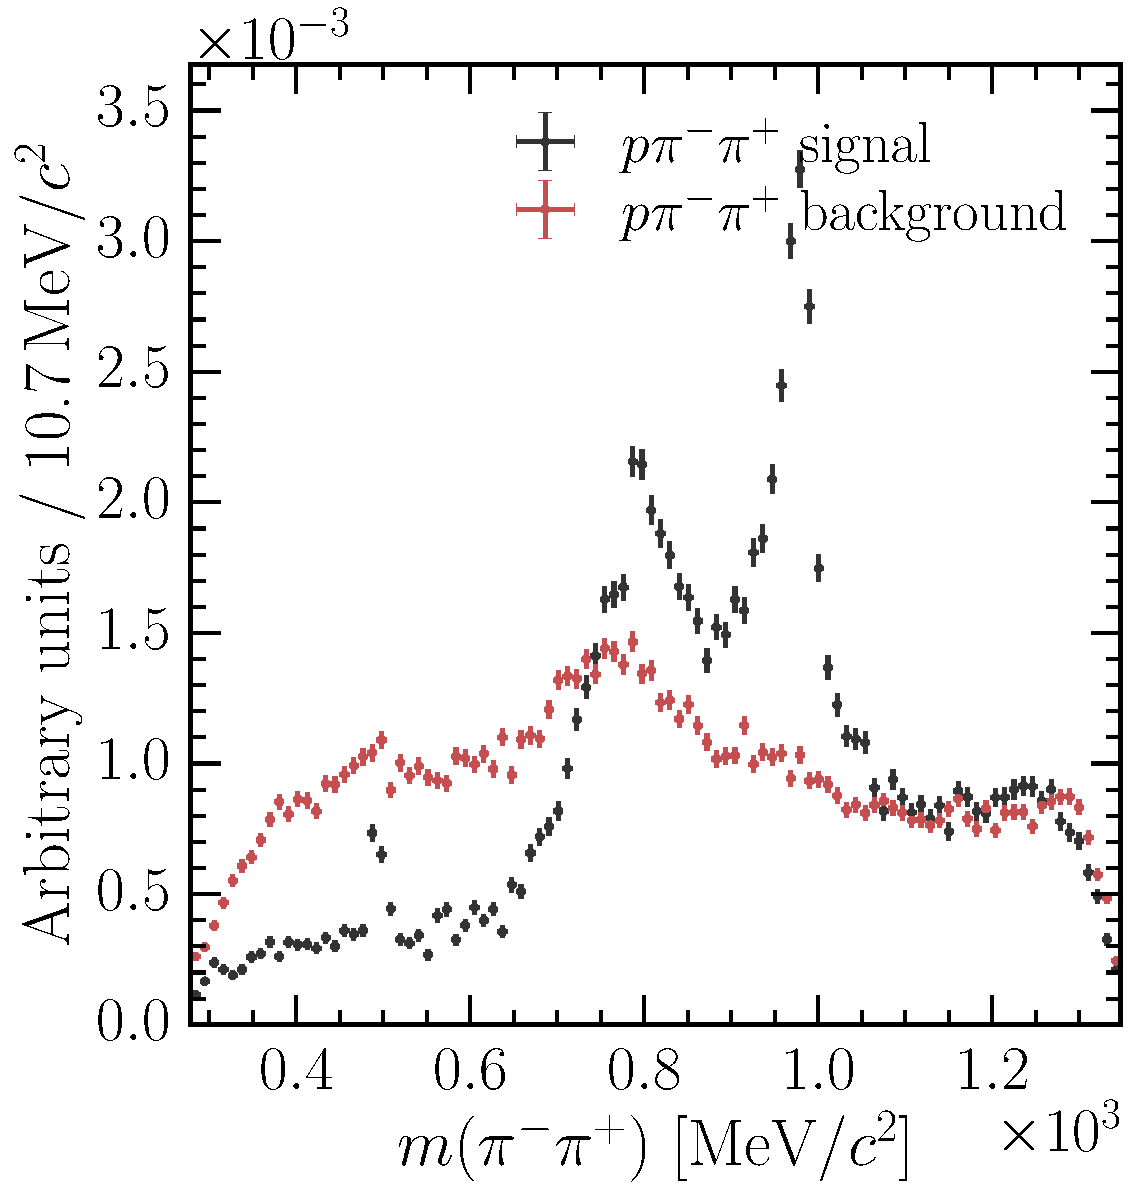
\includegraphics[width=\textwidth]{cpv/selection/LcToppipi_2012_MagDown_Lc_h1_h2_M}
    \caption{Full spectrum}
    \label{fig:cpv:selection:ppipi_ks_cut:full}
  \end{subfigure}
  \begin{subfigure}[b]{0.5\textwidth}
    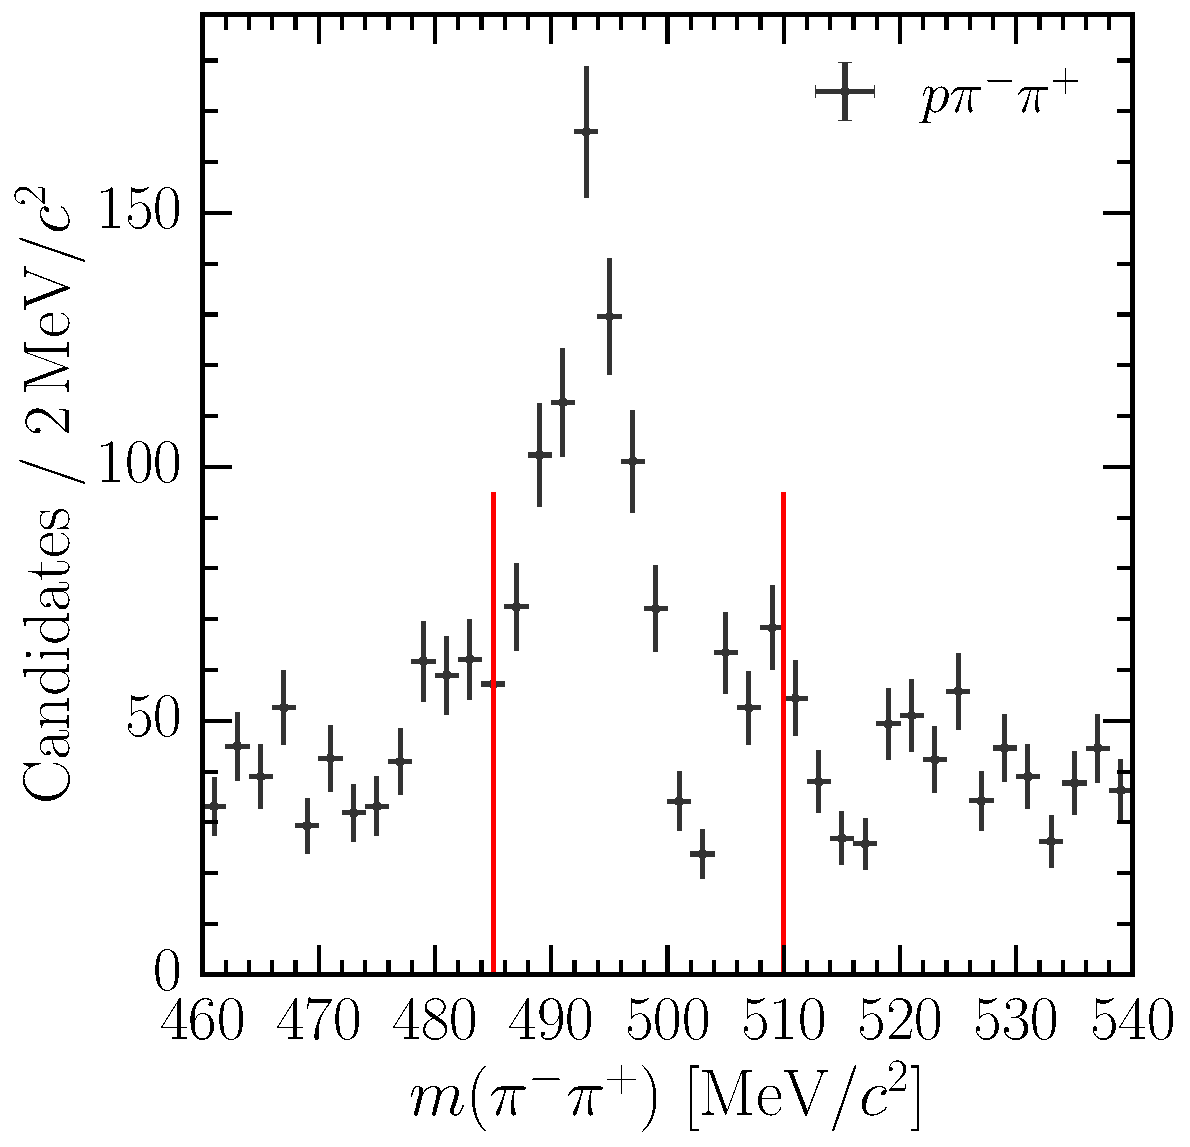
\includegraphics[width=\textwidth]{cpv/selection/LcToppipi_2012_MagDown_Lc_h1_h2_M_zoom}
    \caption{Detail}
    \label{fig:cpv:selection:ppipi_ks_cut:zoom}
  \end{subfigure}
  \caption{%
    Full (\subref*{fig:cpv:selection:ppipi_ks_cut:full}) and zoomed 
    (\subref*{fig:cpv:selection:ppipi_ks_cut:zoom}) mass spectra of the 
    $\Ppiplus\Ppiminus$ pair in the \ppipi\ decay mode, in
    the magnet up 2012 data.
    The background contributions in the black spectra have been statistically
    subtracted, whereas the red spectra have the signal component subtracted.
    The red lines indicate the boundaries of the requirement designed to remove
    the $\Pproton\PKshort$ component of the sample.
    Also visible are the $\rho(770)/\omega(782)$ and $f_{0}(980)$ resonances.
  }
  \label{fig:cpv:selection:ppipi_ks_cut}
\end{figure}

\begin{figure}
  \begin{subfigure}[b]{0.5\textwidth}
    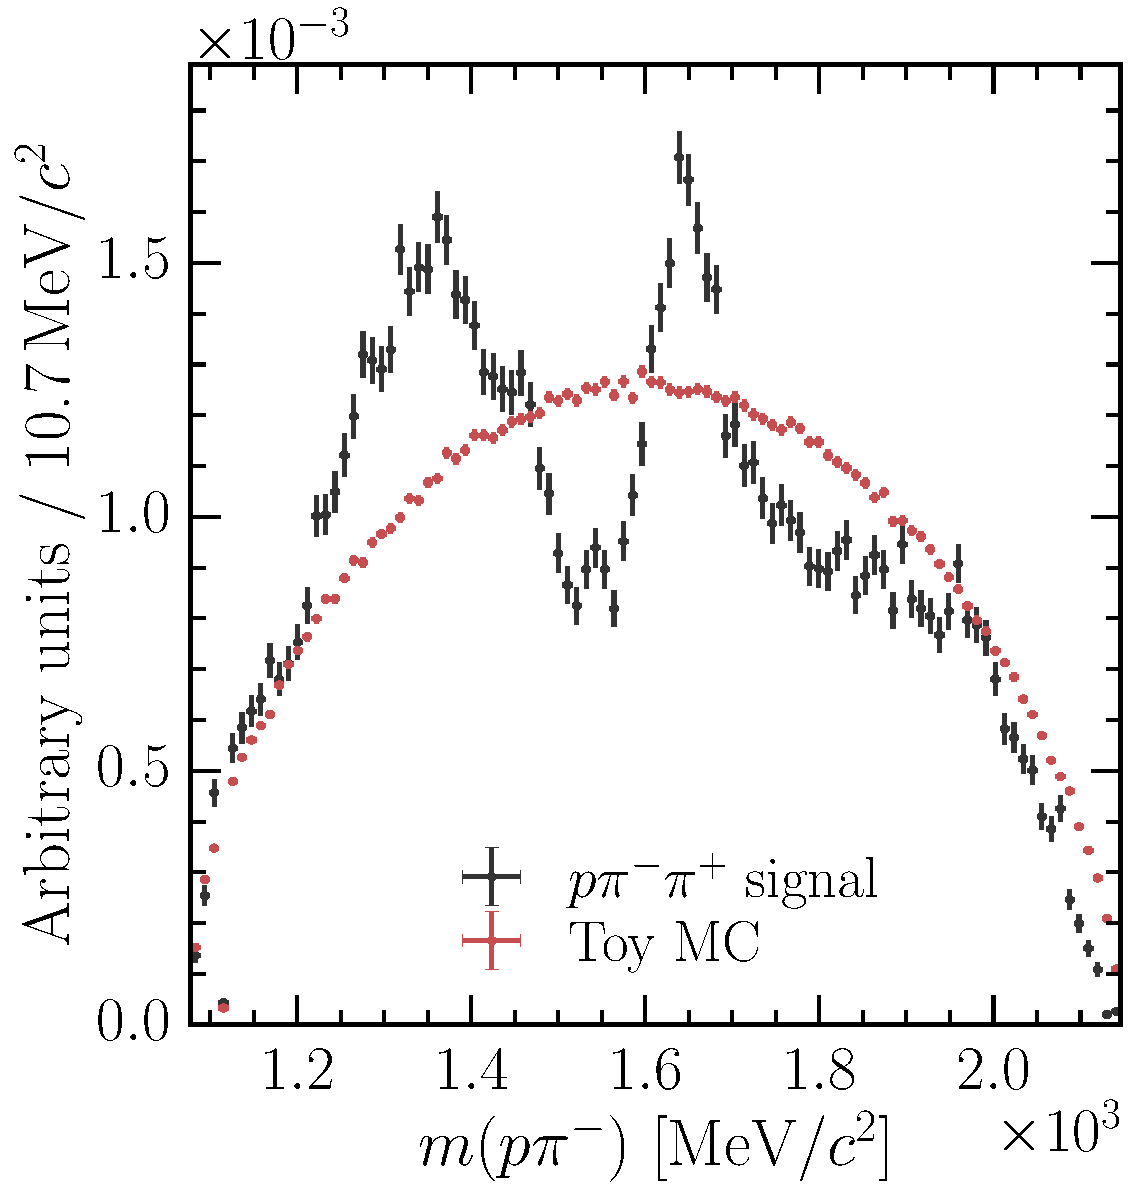
\includegraphics[width=\textwidth]{cpv/selection/LcToppipi_2012_MagDown_Lc_p_h1_M}
    \caption{Full spectrum}
    \label{fig:cpv:selection:ppipi_lambda_cut:full}
  \end{subfigure}
  \begin{subfigure}[b]{0.5\textwidth}
    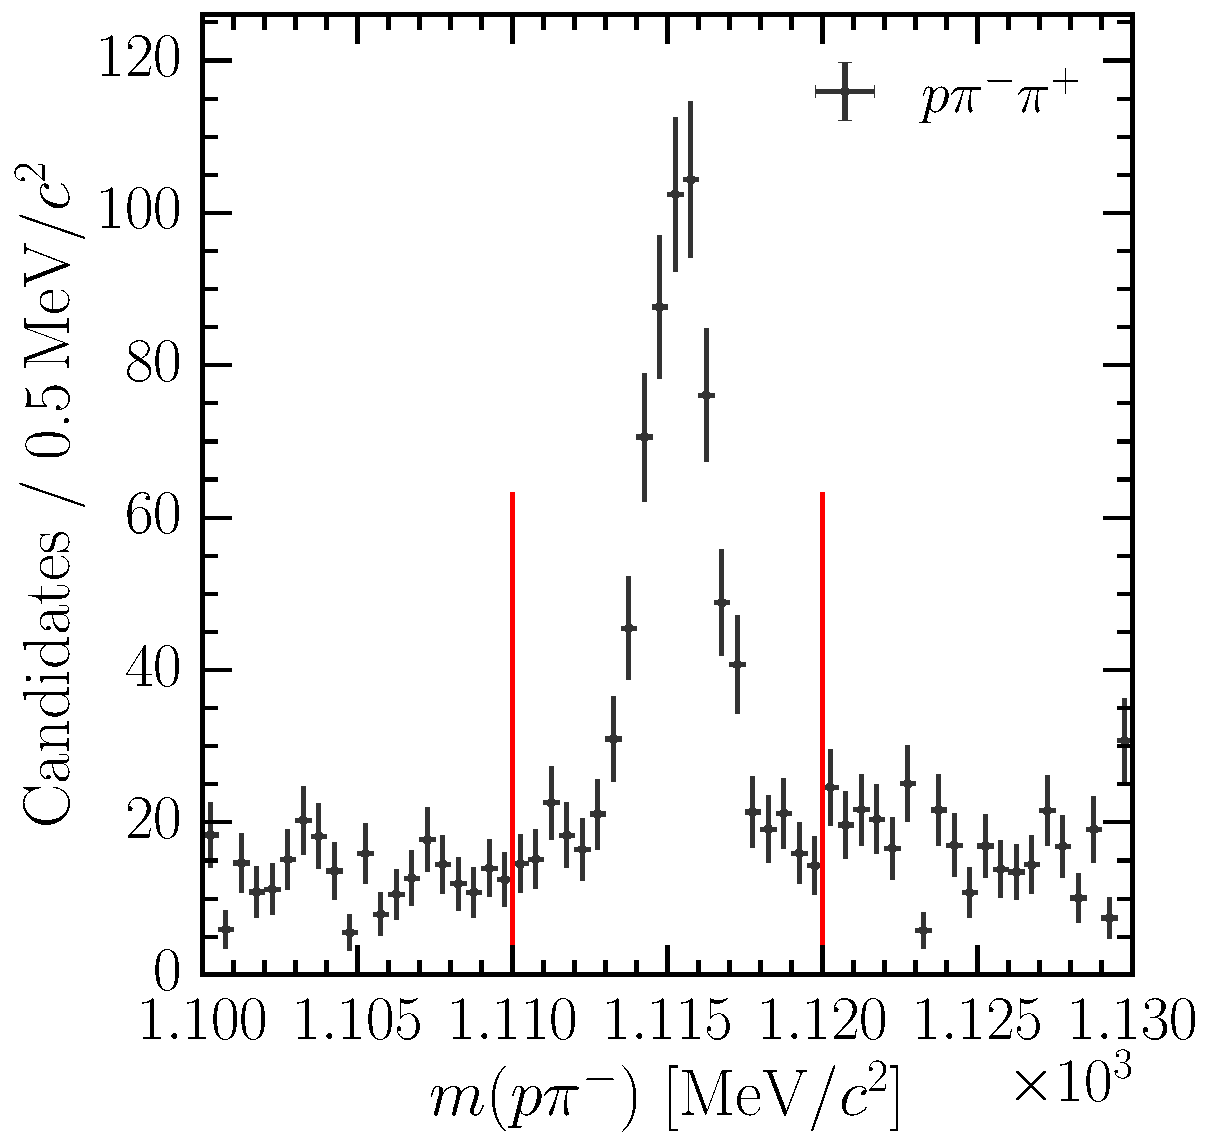
\includegraphics[width=\textwidth]{cpv/selection/LcToppipi_2012_MagDown_Lc_p_h1_M_zoom}
    \caption{Detail}
    \label{fig:cpv:selection:ppipi_lambda_cut:zoom}
  \end{subfigure}
  \caption{%
    Full (\subref*{fig:cpv:selection:ppipi_lambda_cut:full}) and zoomed 
    (\subref*{fig:cpv:selection:ppipi_lambda_cut:zoom}) mass spectra of the 
    $\Pproton\Ppiminus$ pair in the \ppipi\ decay mode, in
    the magnet up 2012 data.
    The background contributions in the black spectra have been statistically
    subtracted, whereas the red spectra have the signal component subtracted.
    The red lines indicate the boundaries of the requirement designed to remove
    the $\PLambda\Ppiplus$ component of the sample.
    The additional features in the $\Pproton\Ppiminus$ spectrum have not been
    identified.
  }
  \label{fig:cpv:selection:ppipi_lambda_cut}
\end{figure}

The largest source of combinatorial background is due to $\PK \to \Pproton$ and
$\Ppi \to \Pproton$ misidentification, as pions and kaons are produced much
more numerously than protons.
The \ac{PID} requirements on the proton, kaon, and pion candidates are
tightened offline.
The \probnn\ family of variables is used, which contains one \probnn\ variable
for each charged particle hypothesis~(\Pproton/\APproton, \PKpm, \Ppipm,
\Pmupm, \Pepm), and is the response of an \ac{ANN} trained to discriminate each
hypothesis from all others.
Input variables to the network include the \ac{DLL} \ac{PID} variables
described in \cref{chap:intro:lhcb:detector:pid}, the track \ptot\ and \pT, and
the total track fit quality and that within each tracking sub-detector.
The \ac{ANN} is trained on a set of truth-matched tracks from a sample of
\ac{MC} generated under 2012 running conditions, and is scaled such that the
signal probability is uniform in the range $\text{\probnn} \in [0, 1]$.

To define a starting point for the \probnn\ cut values, a simultaneous
optimisation of all \ac{PID} requirements was performed by maximising the
signal significance $\sigma$, defined as
\begin{equation}
  \sigma = \frac{%
    \nsig
  }{%
    \sqrt{\nsig + \nbkg}
  },
  \label{eqn:cpv:selection:signal_significance}
\end{equation}
where \nsig\ and \nbkg\ are the signal and background yields in the sample,
measured using the fits described in \cref{chap:cpv:prelim_fits}.
The optimisation showed that the most powerful discriminants between signal and
background were the proton \ac{PID} information, as expected, and the \ac{PID}
information of the kaon or pion with the same charge as the proton.
Applying a selection optimised for the signal significance would then result in
the \ac{PID} requirements being asymmetric in the $\Phm\Php$ meson pair.
As it is known that the \ac{PID} efficiency for a given requirement on a given
particle is dependent on the particle kinematics, as discussed in
\cref{chap:prod:effs:pid}, and that the detection asymmetries also depend on
the same kinematics, the same \ac{PID} cut is applied to both mesons in the
\PLambdac\ final state so as not to induce any additional detection
asymmetries.
The optimal value found for the cut on the meson with opposite sign to the
proton was chosen as the value for the cut on the same-sign meson.
The \ac{PID} requirements made offline on the candidate protons, kaons, and
pions are given in \cref{tab:cpv:selection:pid_cut_values}.

The \phh\ invariant mass distributions after the weak decay vetoes, \ac{PID}
cuts, and \decaytreefitter\ convergence requirements are given in
\cref{fig:cpv:selection:postpid} for the 2012 magnet down dataset.

\begin{table}
  \centering
  \caption{%
    Particle identification requirements made on the \PLambdac\ decay products.
  }
  \label{tab:cpv:selection:pid_cut_values}
  \begin{tabular}{ccc}
    \toprule
    Particle           & Variable  & Requirement \\
    \midrule
    \Pproton/\APproton & \probnnp  & $ > 0.3$    \\
    \PKpm              & \probnnk  & $ > 0.3$    \\
    \Ppipm             & \probnnpi & $ > 0.3$    \\
    \bottomrule
  \end{tabular}
\end{table}

\begin{figure}
  \begin{subfigure}[b]{0.5\textwidth}
    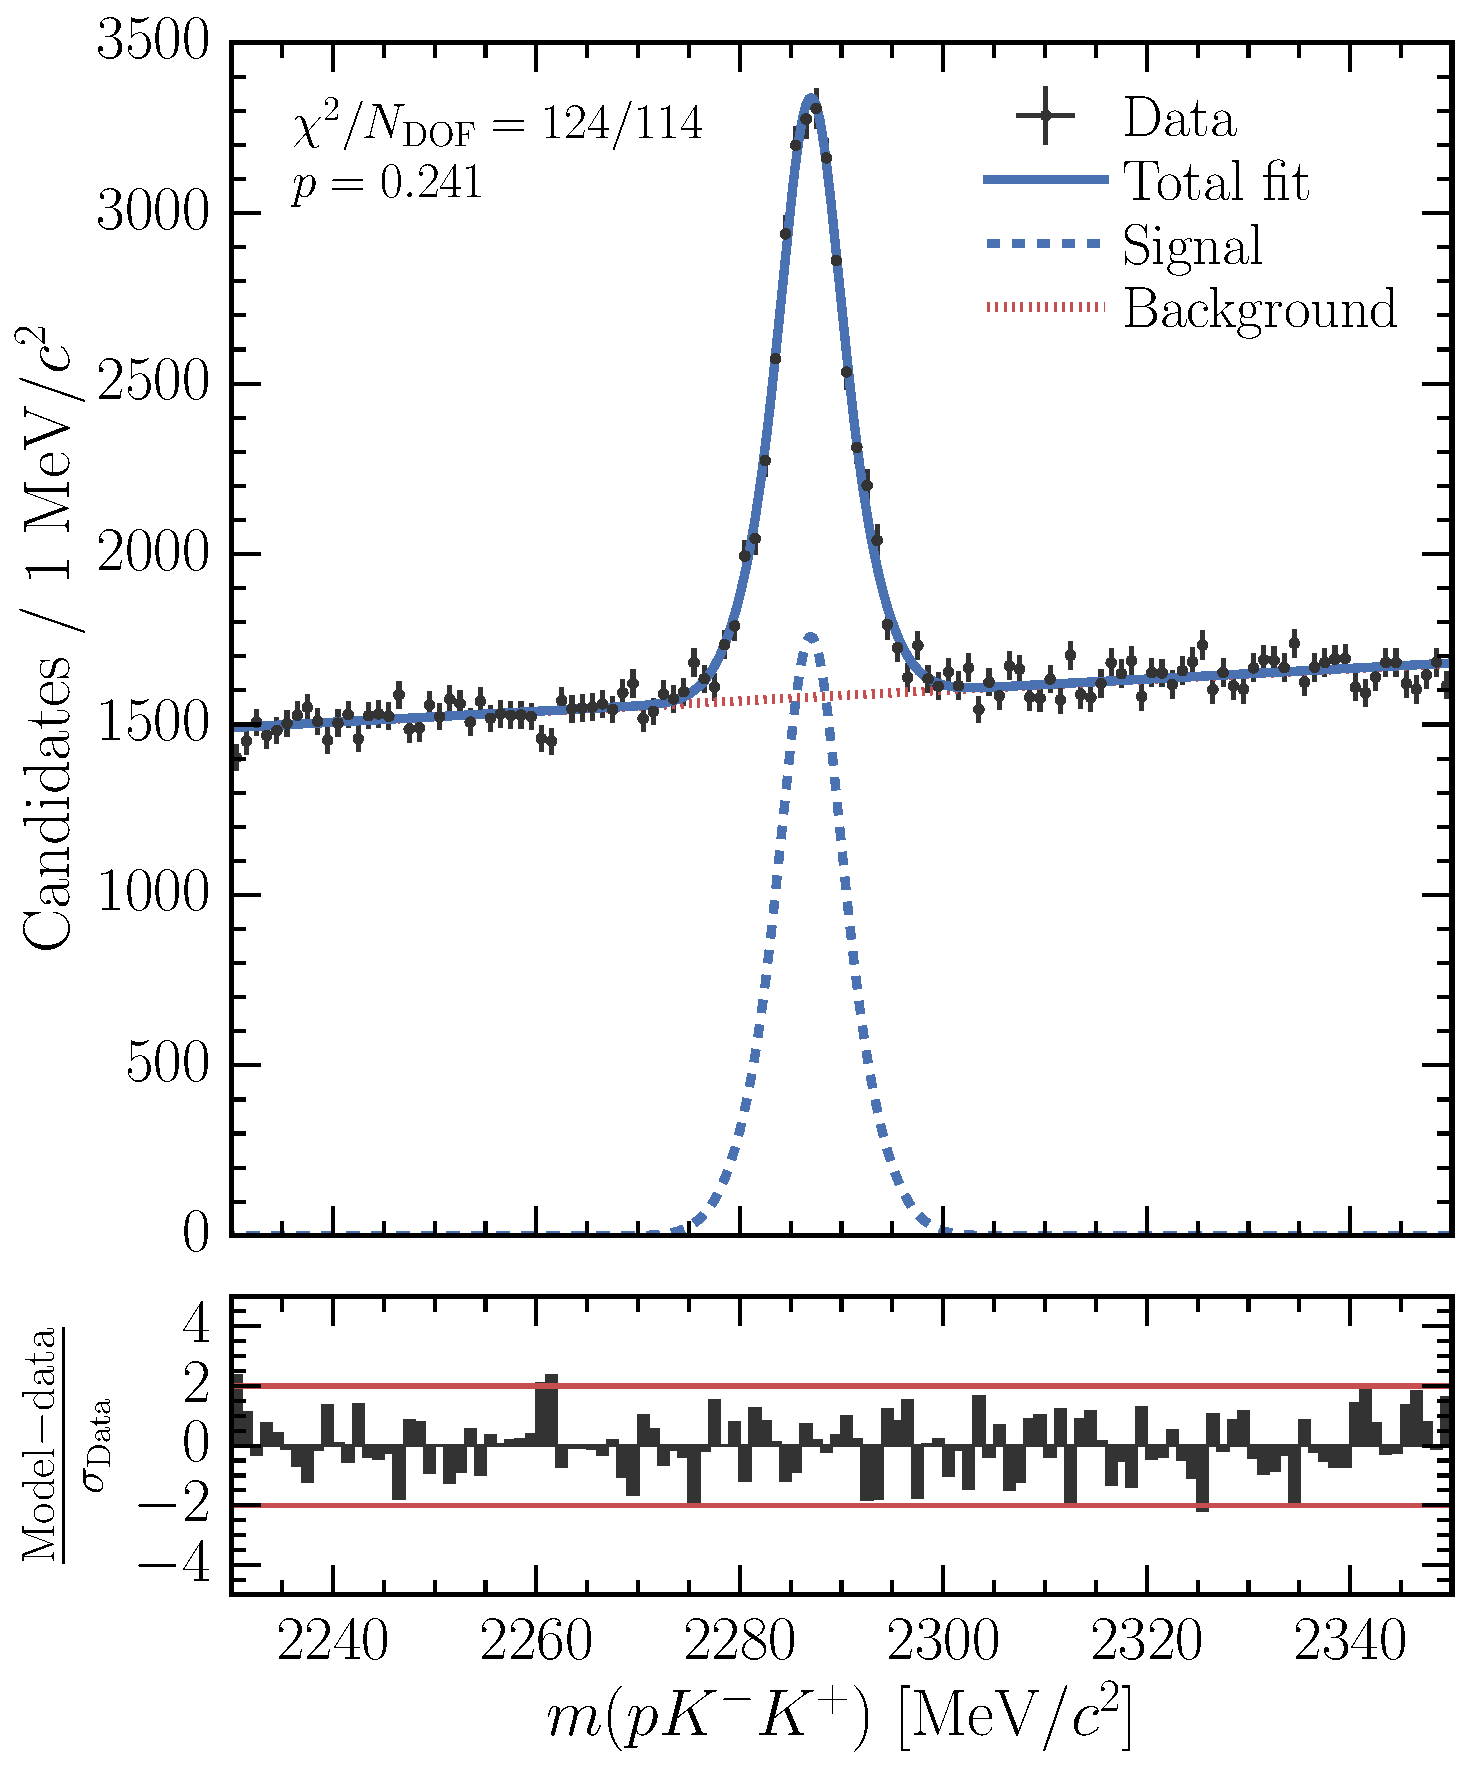
\includegraphics[width=\textwidth]{cpv/selection/fits-offline_stripping_trigger_weak_decay-selection_unweighted_no-simultaneous/LcTopKK_2012_MagDown_fit.pdf}
    \caption{\pKK}
    \label{fig:cpv:selection:postpid:pKK}
  \end{subfigure}
  \begin{subfigure}[b]{0.5\textwidth}
    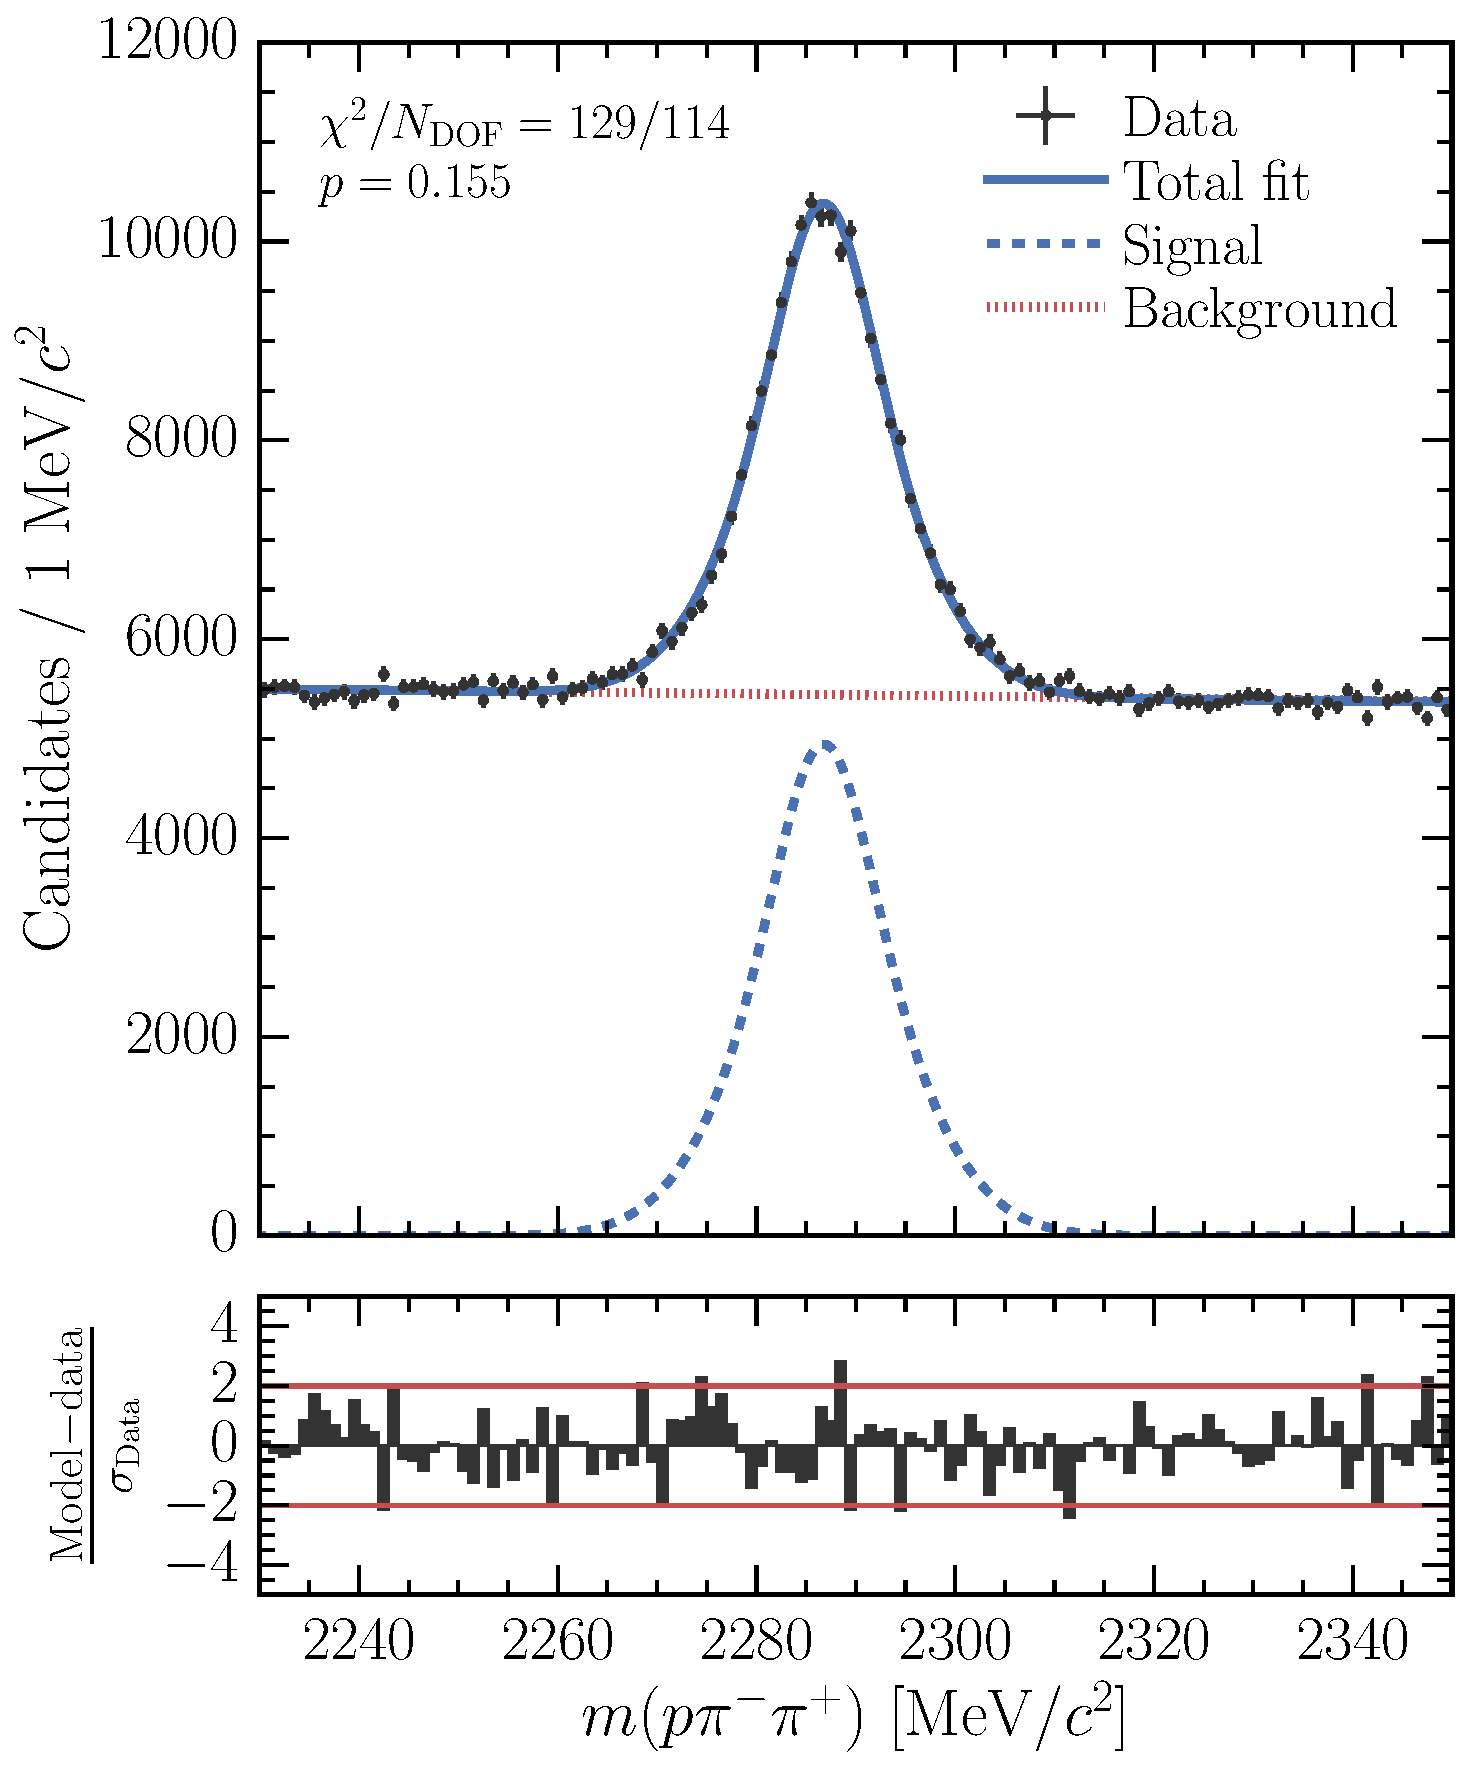
\includegraphics[width=\textwidth]{cpv/selection/fits-offline_stripping_trigger_weak_decay-selection_unweighted_no-simultaneous/LcToppipi_2012_MagDown_fit.pdf}
    \caption{\ppipi}
    \label{fig:cpv:selection:postpid:ppipi}
  \end{subfigure}
  \caption{%
    Fits to the \PLambdac\ mass spectrum in the 2012 magnet down dataset for
    \pKK\ (\subref*{fig:cpv:data:mass:pKK}) and \ppipi\
    (\subref*{fig:cpv:data:mass:ppipi}).
    The stripping, trigger, and \ac{PID} selections are applied, as well as the
    \decaytreefitter\ convergence requirements, and the weak decay vetoes for
    the \ppipi\ data.
    The fit that is overlaid is described in \cref{chap:cpv:prelim_fits}.
  }
  \label{fig:cpv:selection:postpid}
\end{figure}

\section{Background study}
\label{chap:cpv:selection:background_study}

Although \ac{PID} requirements are made on the proton candidate, it is possible
that a meson decay will be misidentified as a \PLambdac\ decay.
For example, a \decay{\PDsplus}{\PKminus\PKplus\Ppiplus} decay could be
misidentified as \LcTopKK\ if the pion is assigned the proton mass hypothesis
and passes the \ac{PID} cuts.
The presence of any such misidentification (or `mis-ID') can add structures to
the \PLambdac\ mass spectrum, making the signal yield extraction more
challenging.
Such structures may peak near the nominal \PLambdac\ mass and be incorrectly
counted as \PLambdac\ signal.
Additional backgrounds can arise due to the partial reconstruction of
\PLambdac\ decays, which would manifest as a `shoulder' at values of the
\PLambdac\ mass below the signal peak.
As this feature is not seen in the \pKK\ or \ppipi\ mass distributions, shown
in \cref{fig:cpv:selection:postpid}, it is considered insignificant and is not
studied further.

One method of checking for the presence of misidentified decays is by
inspecting three-body mass distributions for different mass hypothesis sets.
For example, by assigning the pion mass to the proton candidate in the \pKK\
sample and inspecting the invariant mass of the $\Ppiplus\PKminus\PKplus$
combination.
A peak near the \PDsplus mass would indicate a contamination of \PDsplus
candidates in the data.

A second way to look for meson backgrounds is to inspect the `momentum
asymmetry' parameter of the proton~\cite{Aaltonen:2011jv,Artuso:2121282}
\begin{equation}
  \beta_{\Pproton} = \frac{-p_{\Pproton} + p_{\Php} + p_{\Phm}}{p_{\Pproton} + p_{\Php} + p_{\Phm}},
  \label{eqn:cpv:selection:background_study:mom_asym}
\end{equation}
where $p_{\Pproton}$ is the momentum of the proton candidate and $p_{h^{\pm}}$
is the momentum of the $h^{\pm}$ candidate.
Along with the mass of the \PLambdac, this fully parameterises the mass of the
$\phh$ system under different hypotheses, and so one can infer the presence of
meson backgrounds by inspecting the $\beta_{\Pproton}$--$m(\phh)$ plane.
As the relationship between $m(\phh)$, $\beta_{\Pproton}$, and the three-body
mass under the background hypothesis is known, contours of the expected mis-ID
shape can be drawn on this plane and compared with the data.

Throughout this \lcnamecref{chap:cpv:selection:background_study}, the variables
shown are not computed using any information from the \decaytreefitter\
algorithm described in \cref{chap:cpv:data}.

\subsection{Exchanging mass hypotheses}
\label{chap:cpv:selection:background_study:mass_hypo}

\Cref{fig:cpv:selection:background_study:pKK_meson} shows the three-body mass
distributions in the 2012 magnet down \pKK\ data for several mass hypothesis
sets, where each set does not contain the proton mass hypothesis.
\Cref{fig:cpv:selection:background_study:pKK_baryon} shows the same, but where
each set does contain the proton mass hypothesis.
The two figures show the charm meson and charm baryon background contributions.
\Cref{fig:cpv:selection:background_study:ppipi_meson,fig:cpv:selection:background_study:ppipi_baryon}
show the same but for the 2012 magnet down \ppipi\ data.

The distributions from the \pKK\ data show contributions from
\decay{\PDplus}{\PKplus\PKminus\Ppiplus},
\decay{\PDsplus}{\PKplus\PKminus\Ppiplus}, and
\decay{\PLambdac}{\Pproton\PKminus\Ppiplus} decays.
The \ppipi\ data show \decay{\PDplus}{\PKplus\Ppiminus\Ppiplus},
\decay{\PDplus}{\PKplus\PKminus\Ppiplus},
\decay{\PDsplus}{\PKplus\Ppiminus\Ppiplus}, and
\decay{\PDsplus}{\PKplus\PKminus\Ppiplus} contributions.
Each of these backgrounds is removed by vetoing \PLambdac\ candidates whose
wrong-mass value falls within \SI{8}{\MeV} of the nominal \PDplus, \PDsplus, or
\PLambdac\ mass~\cite{PDG2014}.

A double misidentification of \pKK\ is present in the \pKK\ data, where the
hypotheses of the nominal proton and nominal kaon with the same charge as the
proton are swapped, visible in
\cref{fig:cpv:selection:background_study:pKK_baryon:lcp_KKp}.
This is not removed from the data, as the distribution of candidates that fall
in the signal region of the swapped hypothesis ($\PKplus\PKminus\Pproton$) have
no irregular structures under the nominal hypothesis (\pKK), as shown in
\cref{fig:cpv:selection:background_study:pKK_lcp_KKp_Lc_M}.

\subsection{Momentum asymmetry}
\label{chap:cpv:selection:background_study:mom_asym}

The momentum asymmetry of the proton is defined in
\cref{eqn:cpv:selection:background_study:mom_asym}.
Along with the mass of the \PLambdac\ under the nominal three-body mass
hypothesis, it fully parameterises alternative three-body hypotheses where the
hypothesis of the proton is changed.
The $\beta_{\Pproton}$--$m(\PLambdac)$ plane then provides an additional handle
on misidentification backgrounds, in addition to the technique described in
\cref{chap:cpv:selection:background_study:mass_hypo}.

\Cref{fig:cpv:selection:background_study:mom_asym:pKK,fig:cpv:selection:background_study:mom_asym:ppipi}
show the $\beta_{\Pproton}$--$m(\PLambdac)$ plane with 2012 magnet down data.
There are distinct contributions from \decay{\PDplus}{\PKplus\PKminus\Ppiplus}
and \decay{\PDsplus}{\PKplus\PKminus\Ppiplus} in the \pKK\ data, and from
\decay{\PDsplus}{\PKplus\Ppiminus\Ppiplus} in the \ppipi\ data.
Also shown are the $\beta_{\Pproton}$--$m(\PLambdac)$ planes after the
misidentification vetoes described in
\cref{chap:cpv:selection:background_study:mass_hypo} have been applied.
No contributions beyond those given in
\cref{chap:cpv:selection:background_study:mass_hypo} are seen.

\begin{figure}
  \begin{subfigure}[b]{0.3\textwidth}
    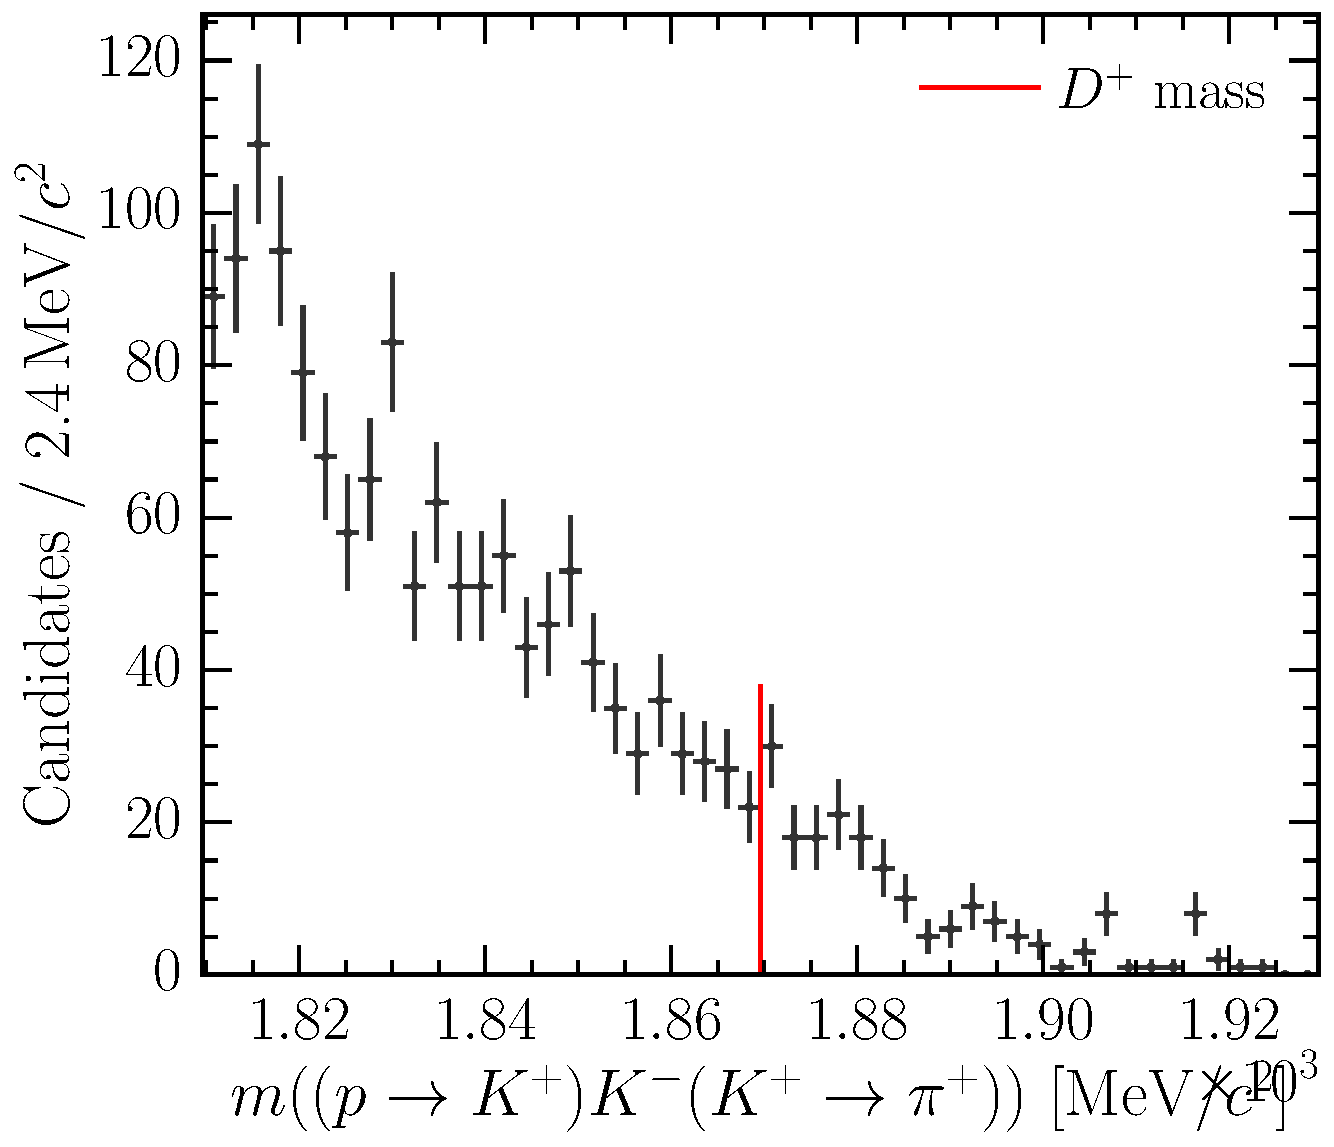
\includegraphics[width=\textwidth]{cpv/selection/background_study/pKK/LcTopKK_2012_MagDown_Dp_ppTokp_km_kpTopip}
    \caption{\decay{\PDplus}{\PKplus\PKminus\Ppiplus}}
    \label{fig:cpv:selection:background_study:pKK_meson:dplus_kkpi}
  \end{subfigure}
  \begin{subfigure}[b]{0.3\textwidth}
    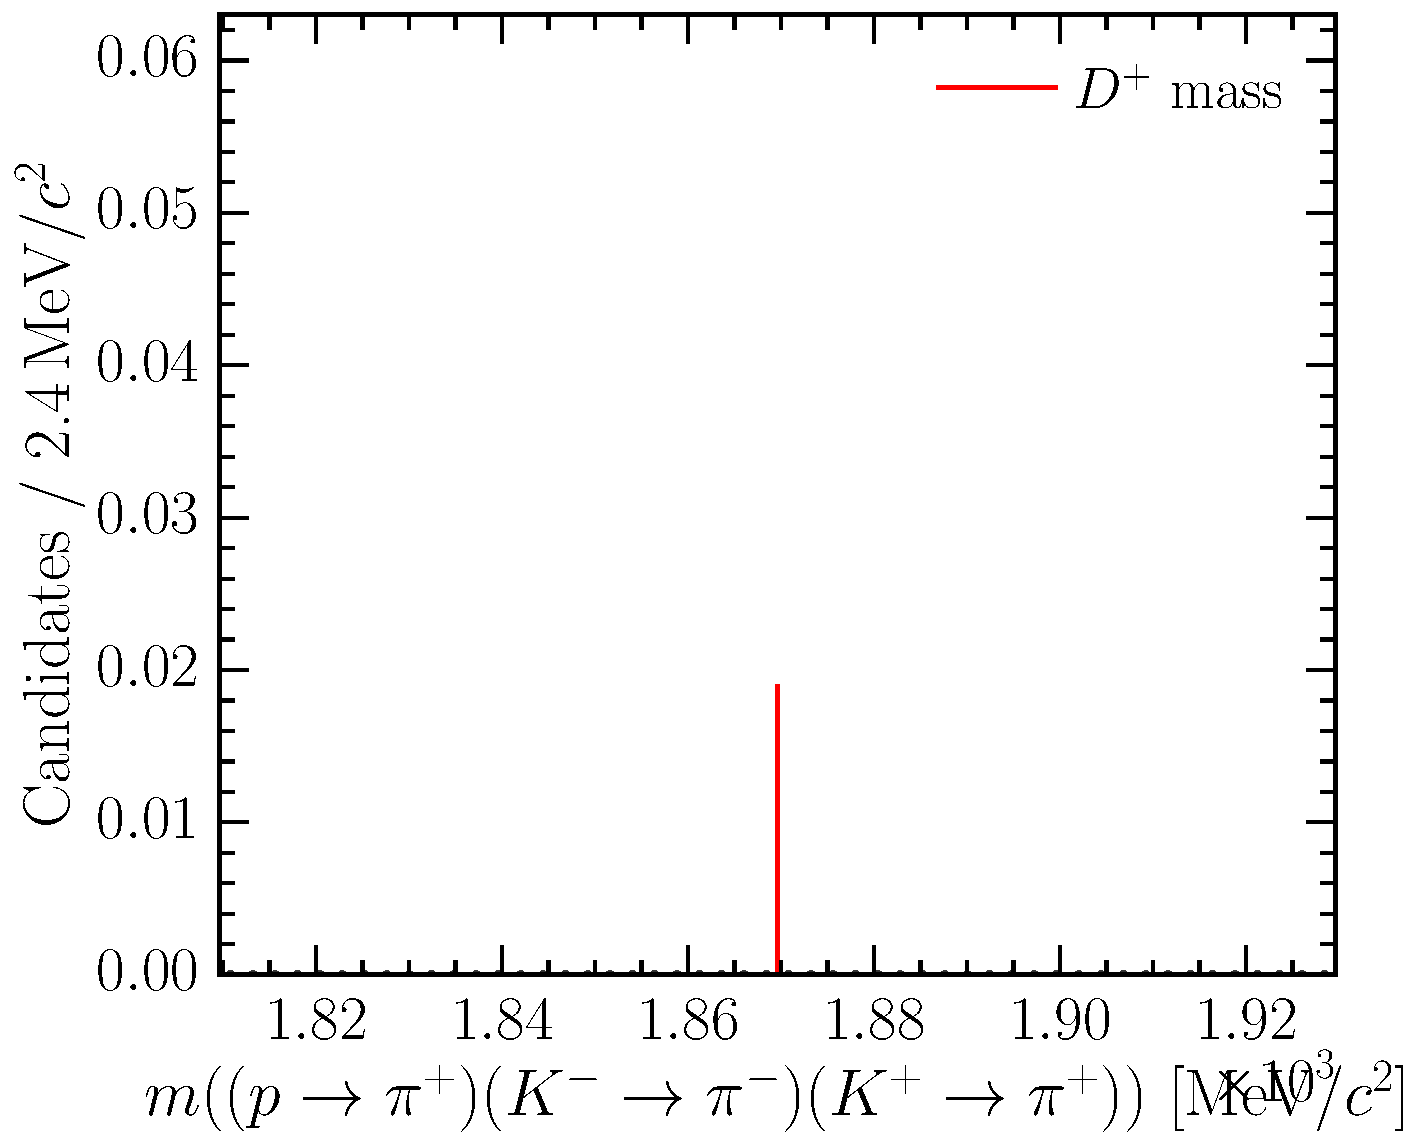
\includegraphics[width=\textwidth]{cpv/selection/background_study/pKK/LcTopKK_2012_MagDown_Dp_ppTopip_kmTopim_kpTopip}
    \caption{\decay{\PDplus}{\Ppiplus\Ppiminus\Ppiplus}}
    \label{fig:cpv:selection:background_study:pKK_meson:dplus_pipipi}
  \end{subfigure}
  \begin{subfigure}[b]{0.3\textwidth}
    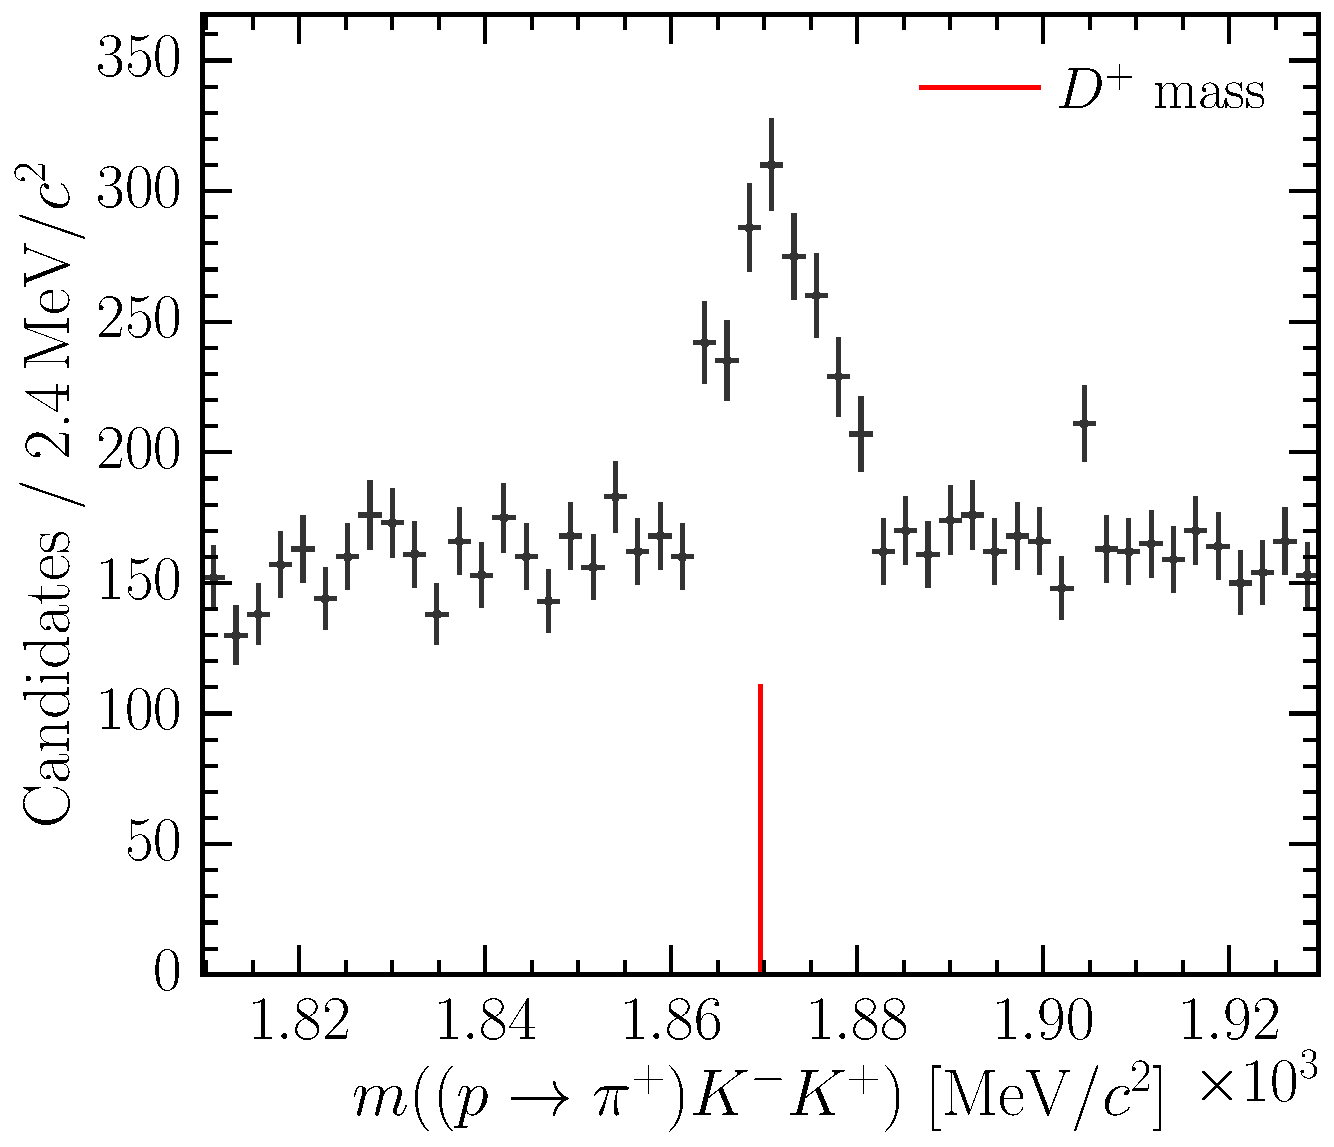
\includegraphics[width=\textwidth]{cpv/selection/background_study/pKK/LcTopKK_2012_MagDown_Dp_ppTopip_km_kp}
    \caption{\decay{\PDplus}{\Ppiplus\PKminus\PKplus}}
    \label{fig:cpv:selection:background_study:pKK_meson:dplus_pikk}
  \end{subfigure}

  \begin{subfigure}[b]{0.3\textwidth}
    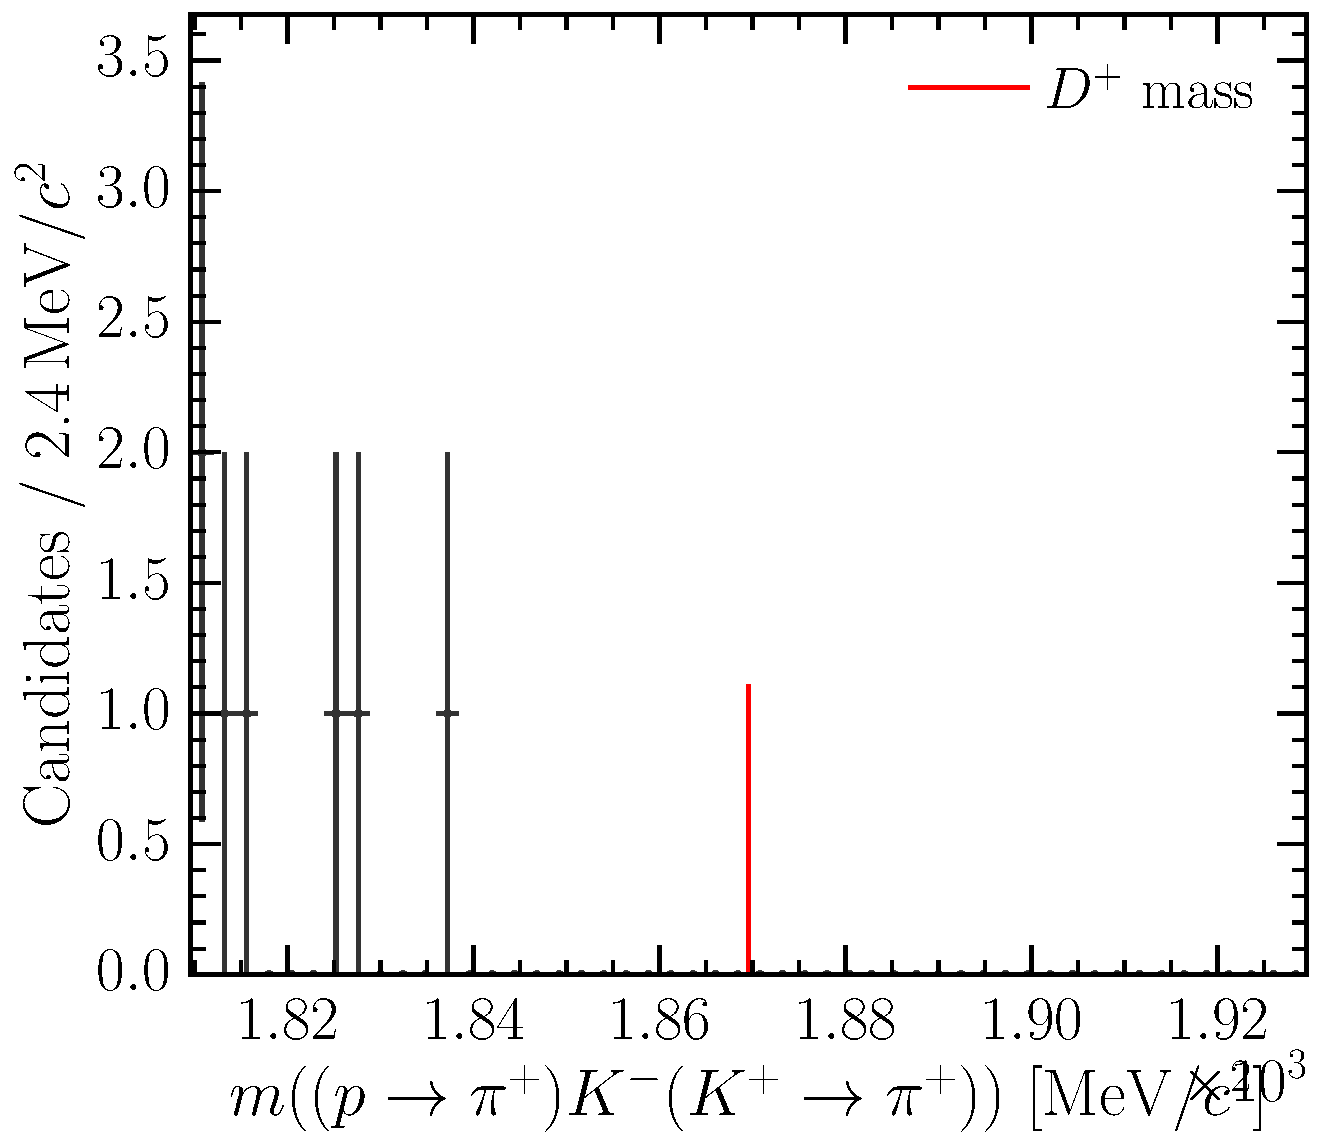
\includegraphics[width=\textwidth]{cpv/selection/background_study/pKK/LcTopKK_2012_MagDown_Dp_ppTopip_km_kpTopip}
    \caption{\decay{\PDplus}{\Ppiplus\PKminus\Ppiplus}}
    \label{fig:cpv:selection:background_study:pKK_meson:dplus_pikpi}
  \end{subfigure}
  \begin{subfigure}[b]{0.3\textwidth}
    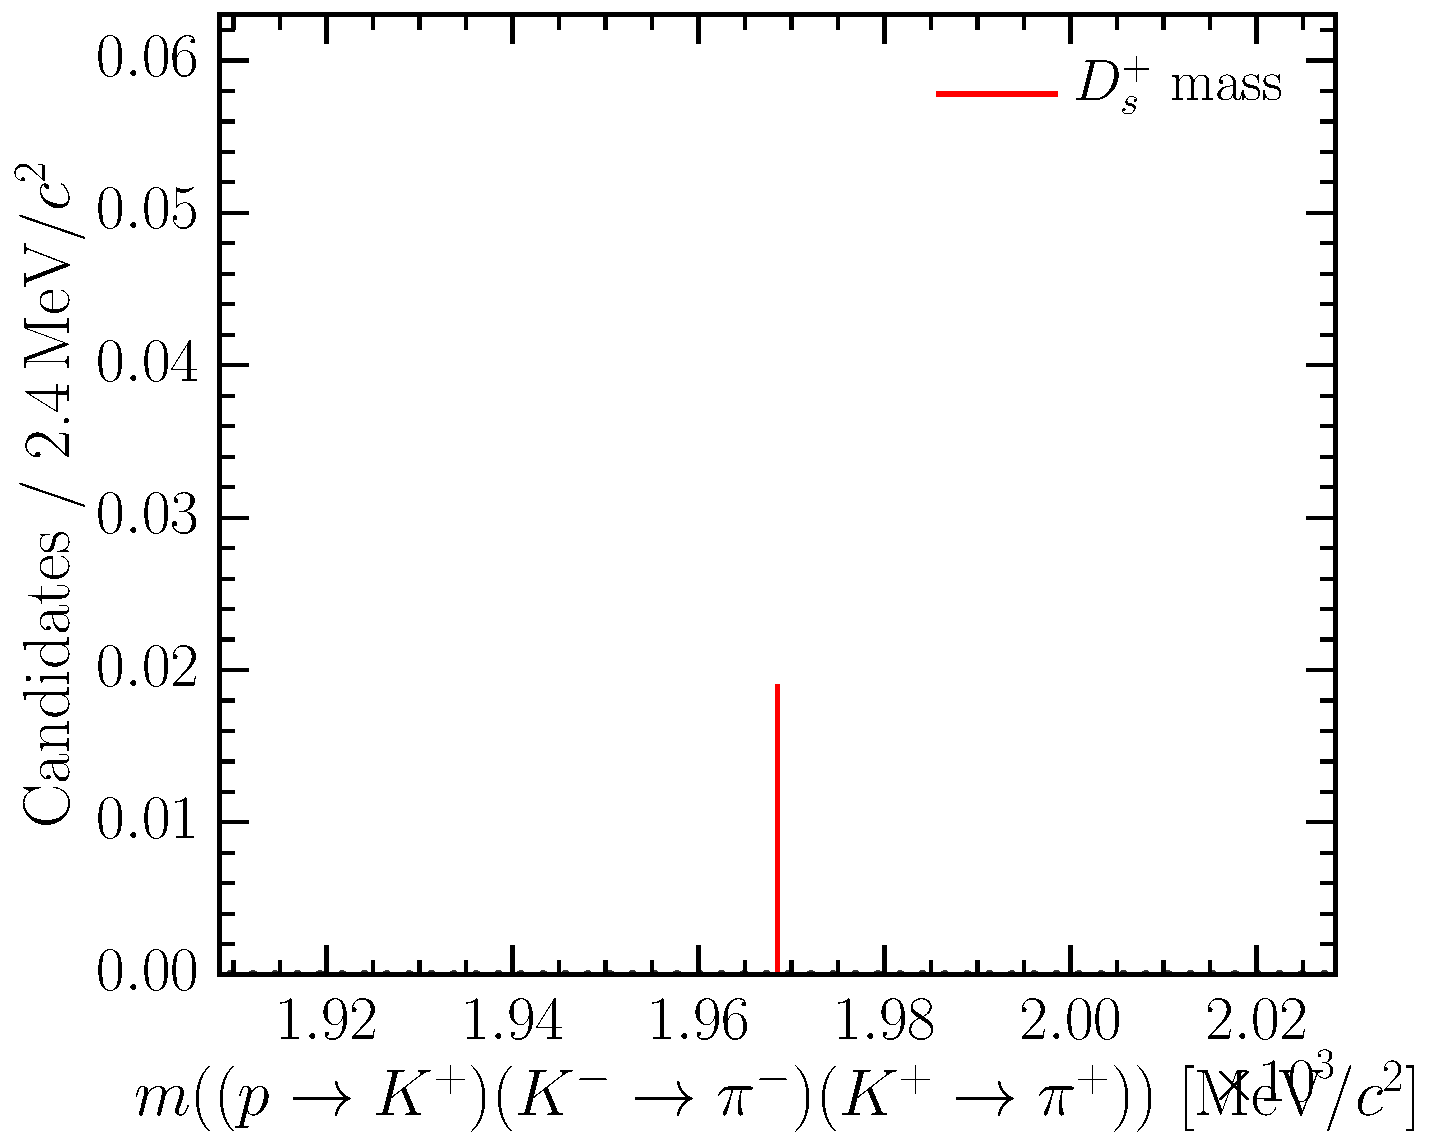
\includegraphics[width=\textwidth]{cpv/selection/background_study/pKK/LcTopKK_2012_MagDown_Ds_ppTokp_kmTopim_kpTopip}
    \caption{\decay{\PDsplus}{\PKplus\Ppiminus\Ppiplus}}
    \label{fig:cpv:selection:background_study:pKK_meson:dsplus_Kpipi}
  \end{subfigure}
  \begin{subfigure}[b]{0.3\textwidth}
    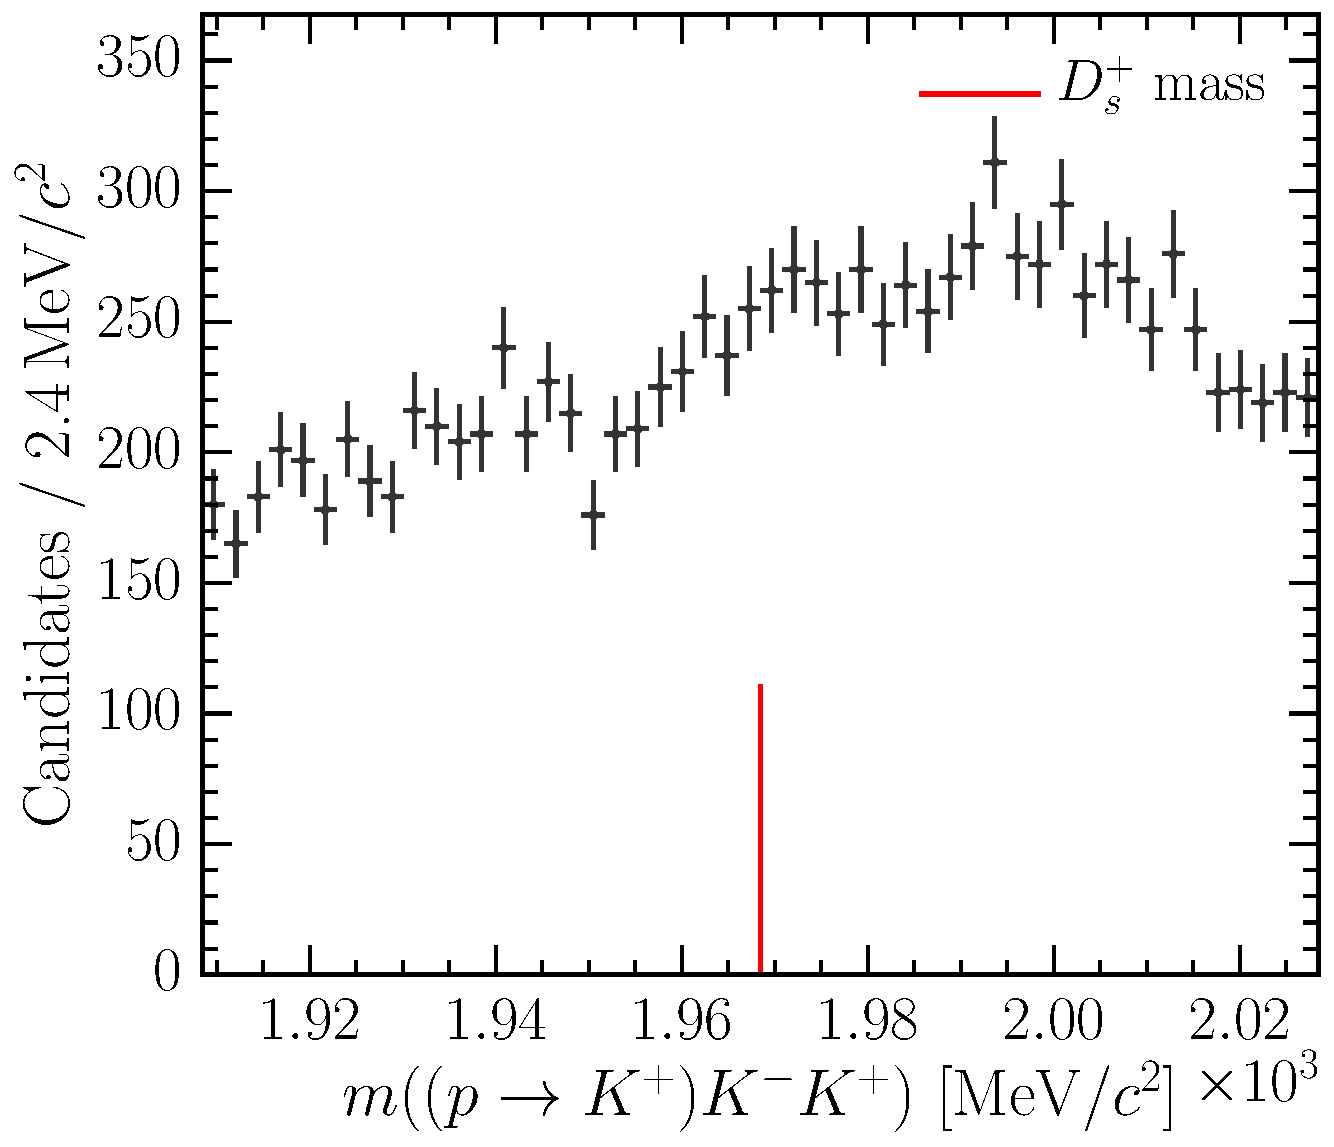
\includegraphics[width=\textwidth]{cpv/selection/background_study/pKK/LcTopKK_2012_MagDown_Ds_ppTokp_km_kp}
    \caption{\decay{\PDsplus}{\PKplus\PKminus\PKplus}}
    \label{fig:cpv:selection:background_study:pKK_meson:dsplus_KKK}
  \end{subfigure}

  \begin{subfigure}[b]{0.3\textwidth}
    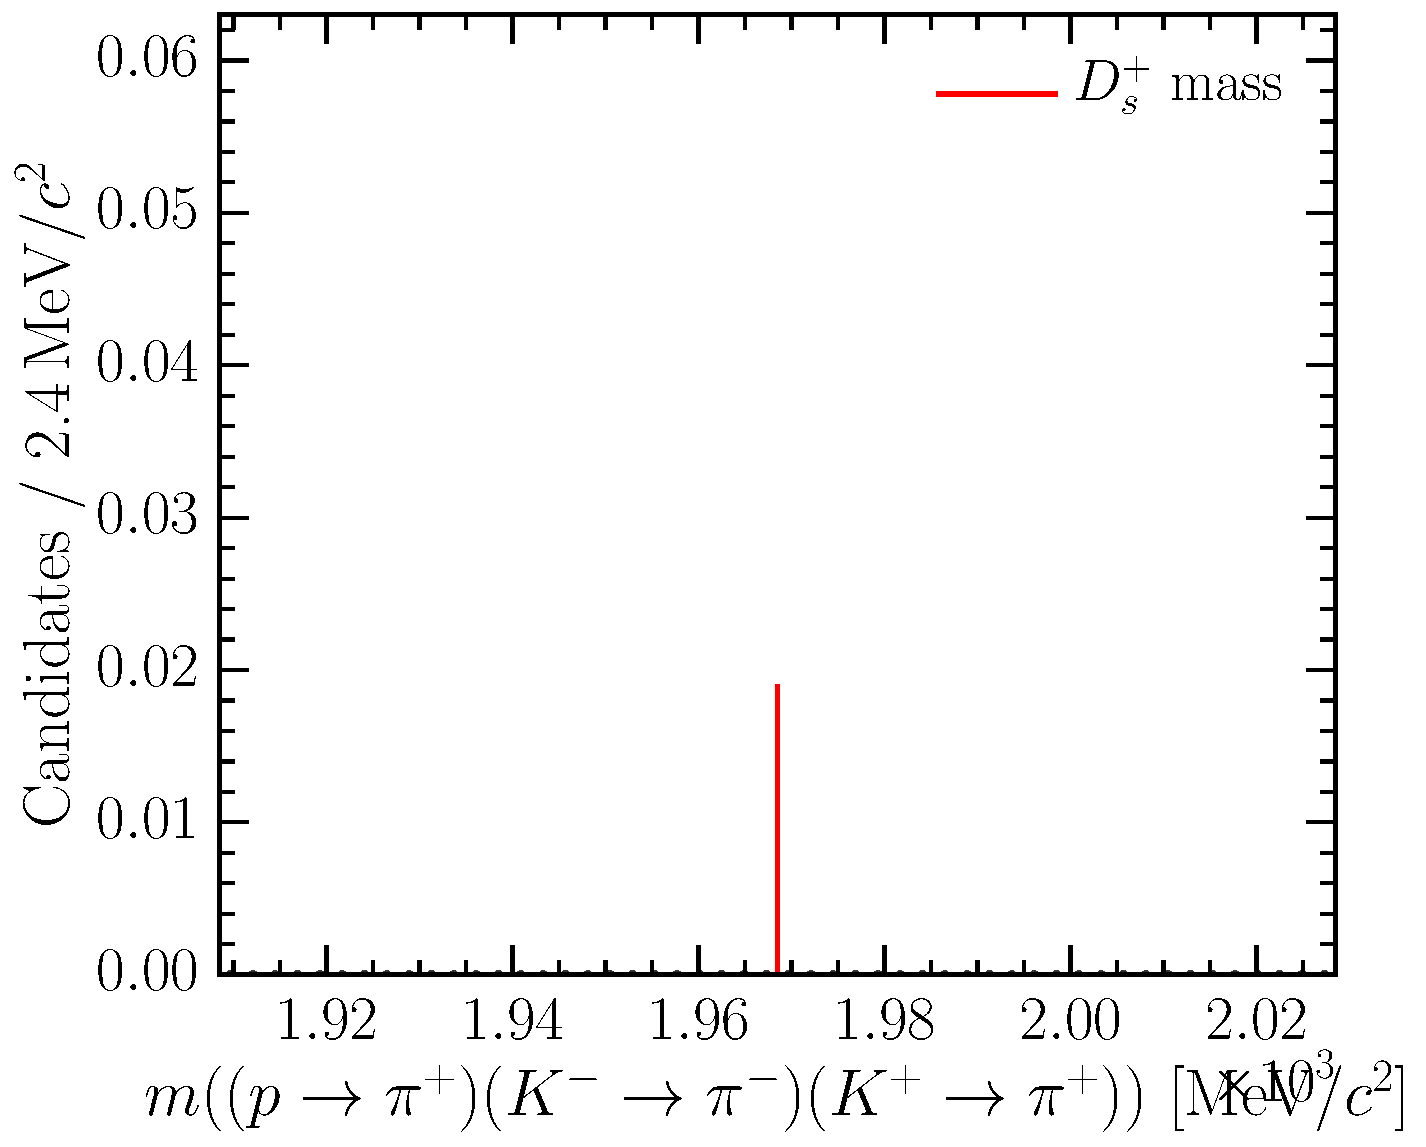
\includegraphics[width=\textwidth]{cpv/selection/background_study/pKK/LcTopKK_2012_MagDown_Ds_ppTopip_kmTopim_kpTopip}
    \caption{\decay{\PDsplus}{\Ppiplus\Ppiminus\Ppiplus}}
    \label{fig:cpv:selection:background_study:pKK_meson:dsplus_pipipi}
  \end{subfigure}
  \begin{subfigure}[b]{0.3\textwidth}
    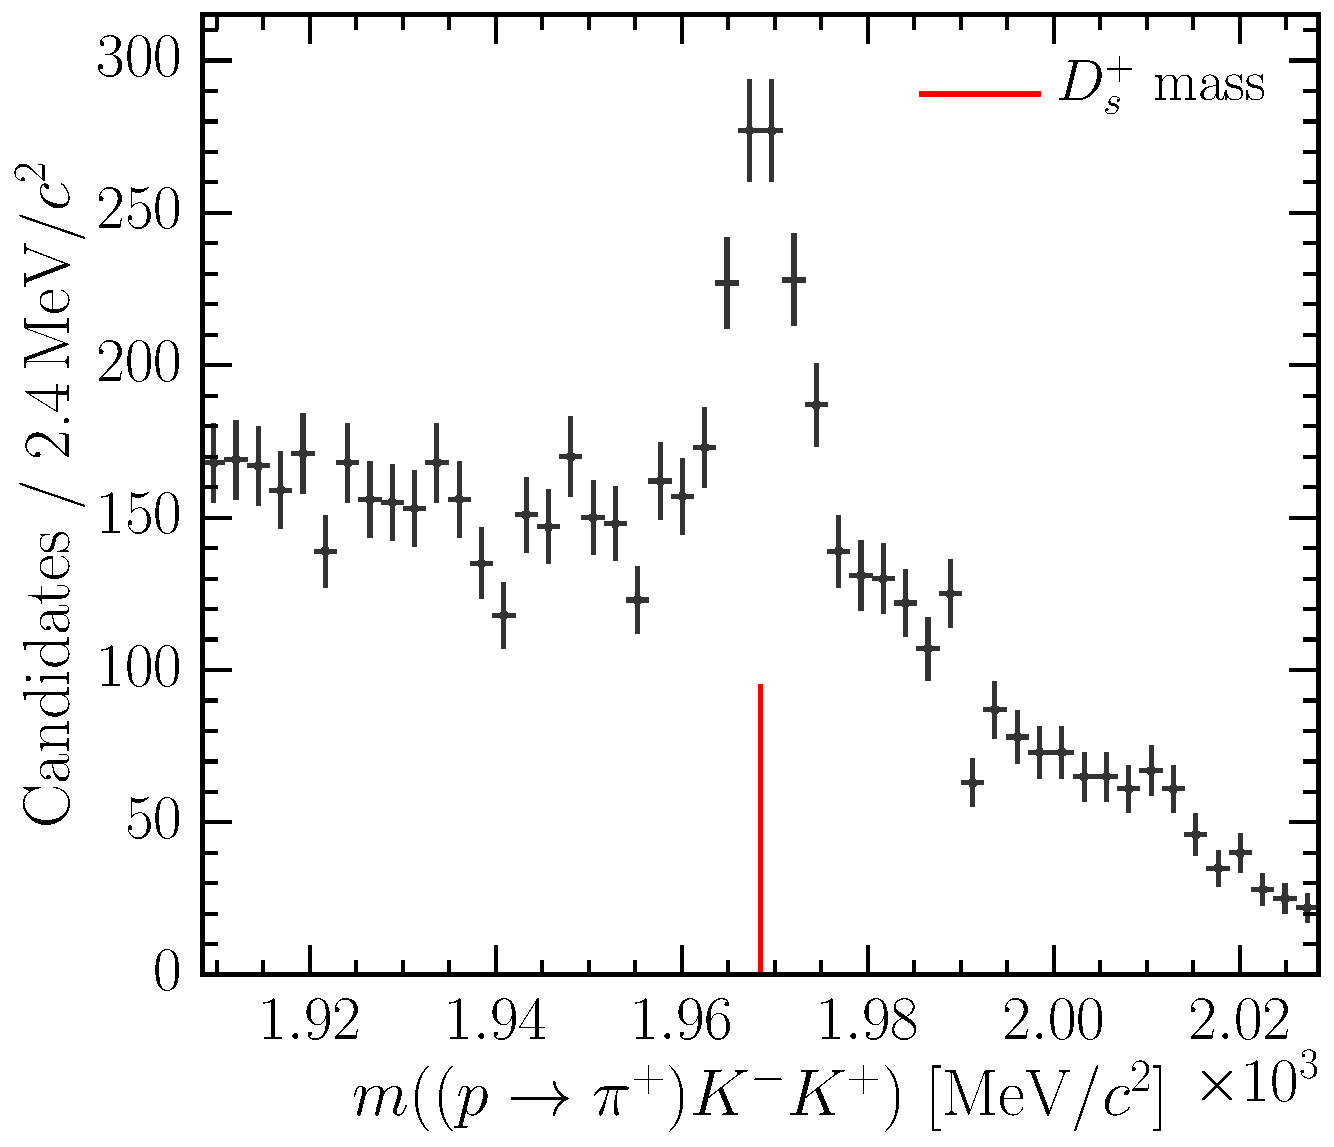
\includegraphics[width=\textwidth]{cpv/selection/background_study/pKK/LcTopKK_2012_MagDown_Ds_ppTopip_km_kp}
    \caption{\decay{\PDsplus}{\Ppiplus\PKminus\PKplus}}
    \label{fig:cpv:selection:background_study:pKK_meson:dsplus_piKK}
  \end{subfigure}

  \caption{%
    Wrong-mass distributions obtained when changing the mass hypotheses of the
    fully selected \PLambdac\ children in the \pKK\ mode, where no child is
    assigned the proton mass hypothesis.
    The $x$-axis on each sub-figure shows the substitutions that have been
    made.
    For example, the ${(\Pproton \to \Ppiplus)(\PKminus \to \Ppiminus)\PKplus}$ distribution is
    where the nominal proton candidate has been assigned the pion mass
    hypothesis, and the nominal kaon with opposite charge to the proton has
    been also assigned the pion hypothesis.
    The vertical red lines indicate the nominal mass of the misidentified 
    particle under study.
    Only the 2012 magnet down data is shown.
  }
  \label{fig:cpv:selection:background_study:pKK_meson}
\end{figure}


\begin{figure}
  \begin{subfigure}[b]{0.3\textwidth}
    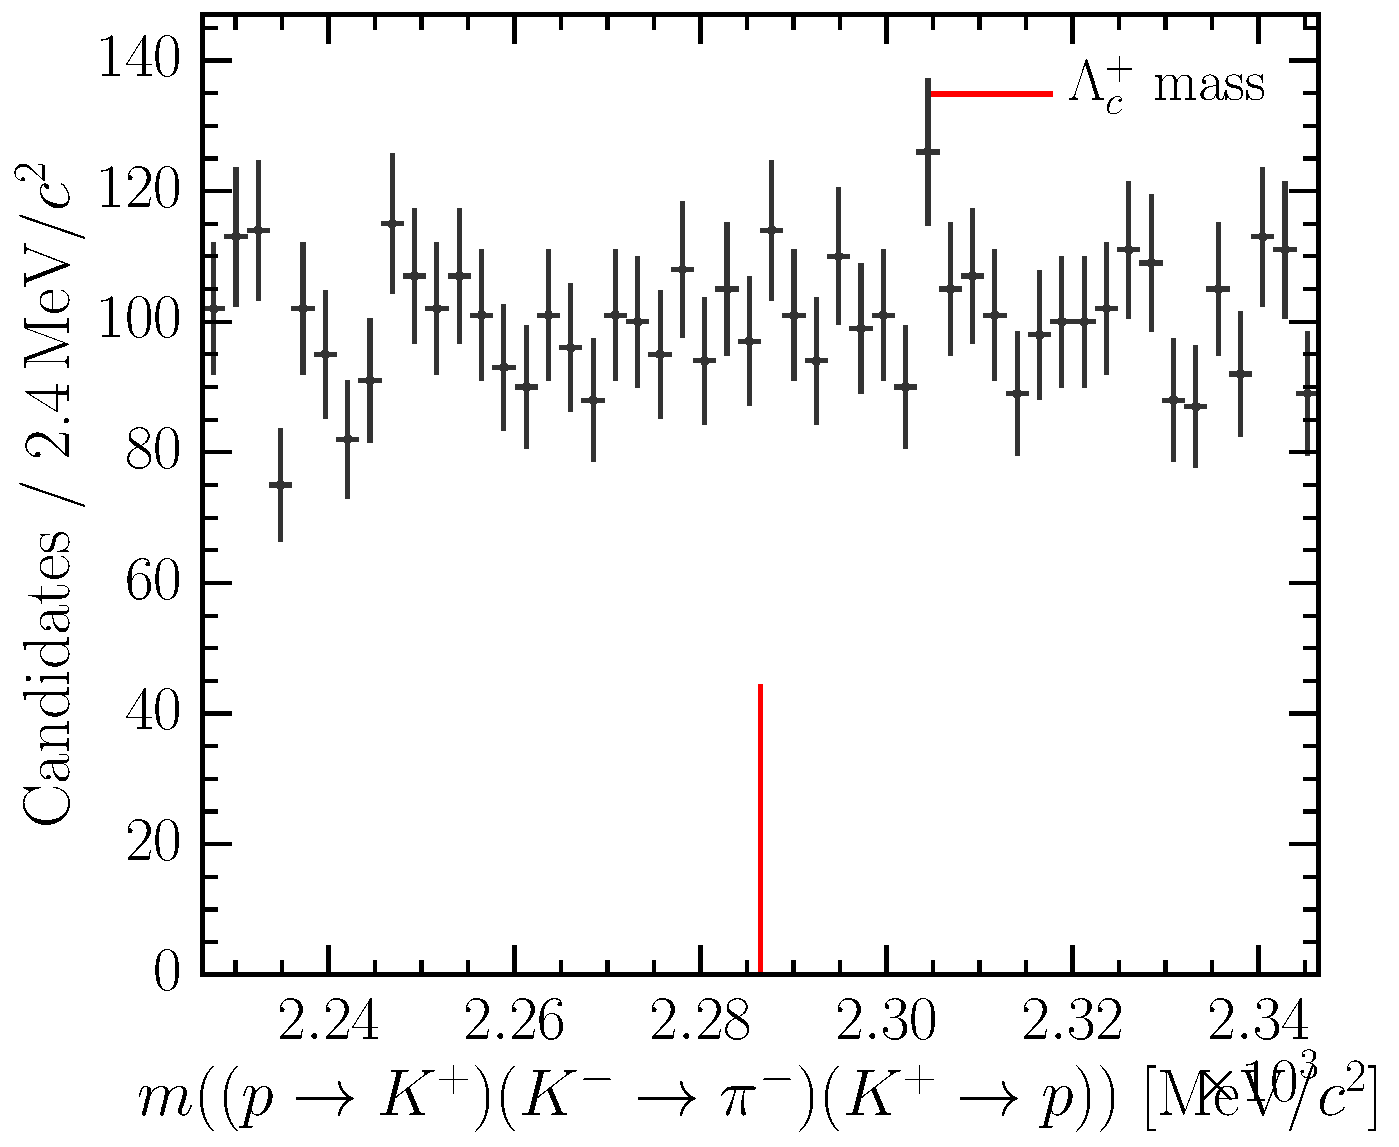
\includegraphics[width=\textwidth]{cpv/selection/background_study/pKK/LcTopKK_2012_MagDown_Lc_ppTokp_kmTopim_kpTopp}
    \caption{\decay{\PLambdac}{\PKplus\Ppiminus\Pproton}}
    \label{fig:cpv:selection:background_study:pKK_baryon:lcp_Kpip}
  \end{subfigure}
  \begin{subfigure}[b]{0.3\textwidth}
    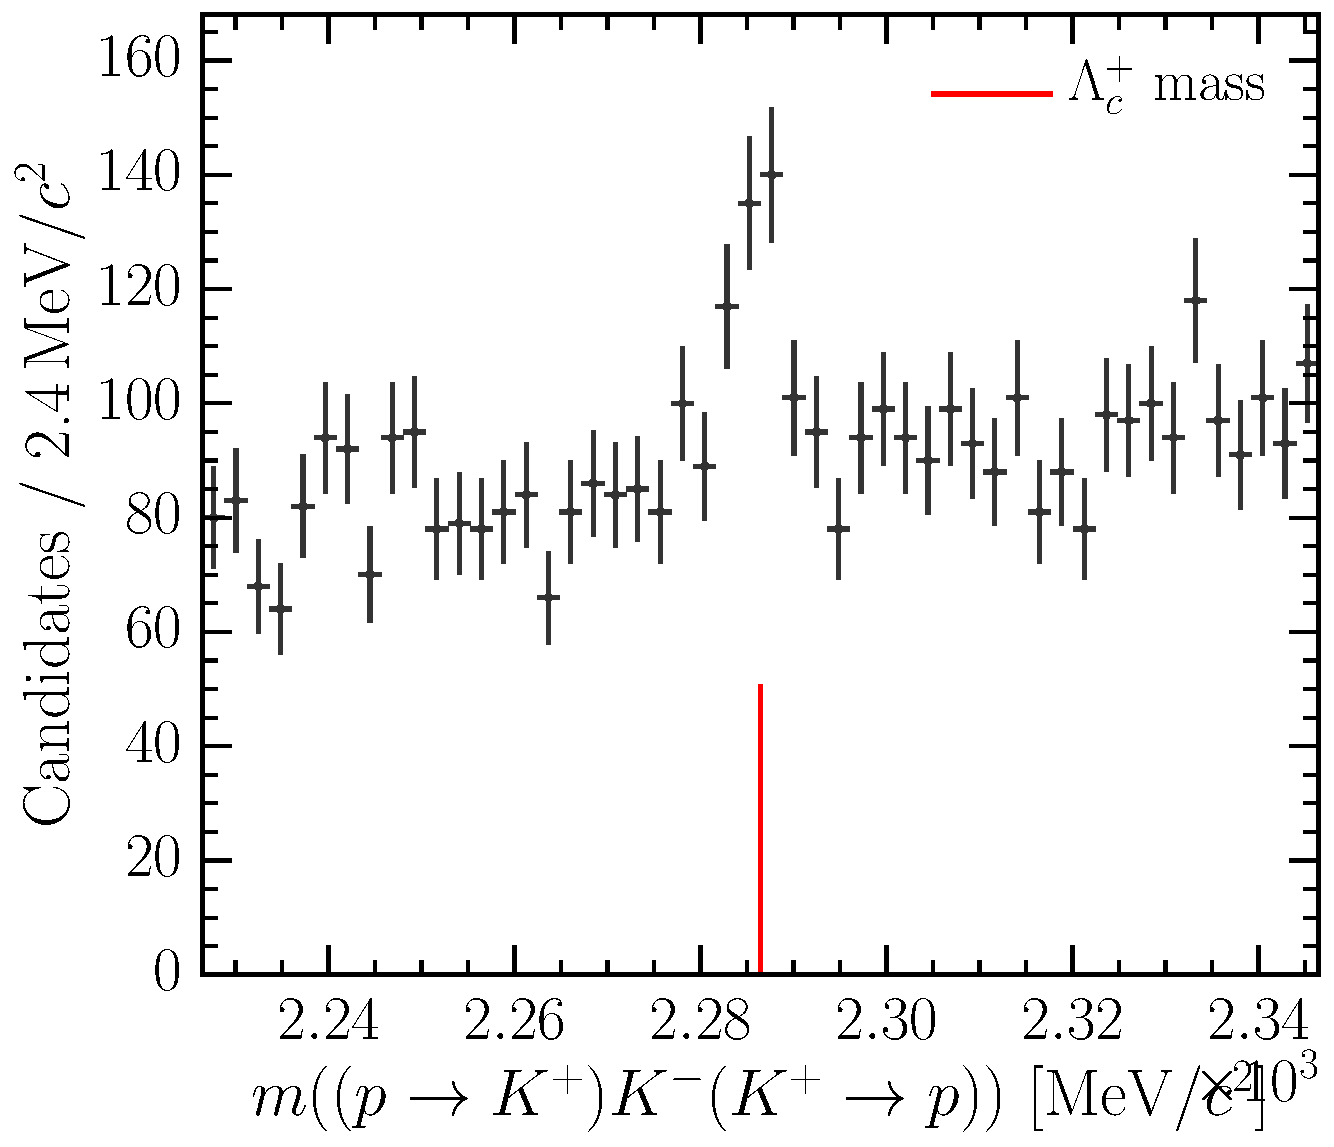
\includegraphics[width=\textwidth]{cpv/selection/background_study/pKK/LcTopKK_2012_MagDown_Lc_ppTokp_km_kpTopp}
    \caption{\decay{\PLambdac}{\PKplus\PKminus\Pproton}}
    \label{fig:cpv:selection:background_study:pKK_baryon:lcp_KKp}
  \end{subfigure}
  \begin{subfigure}[b]{0.3\textwidth}
    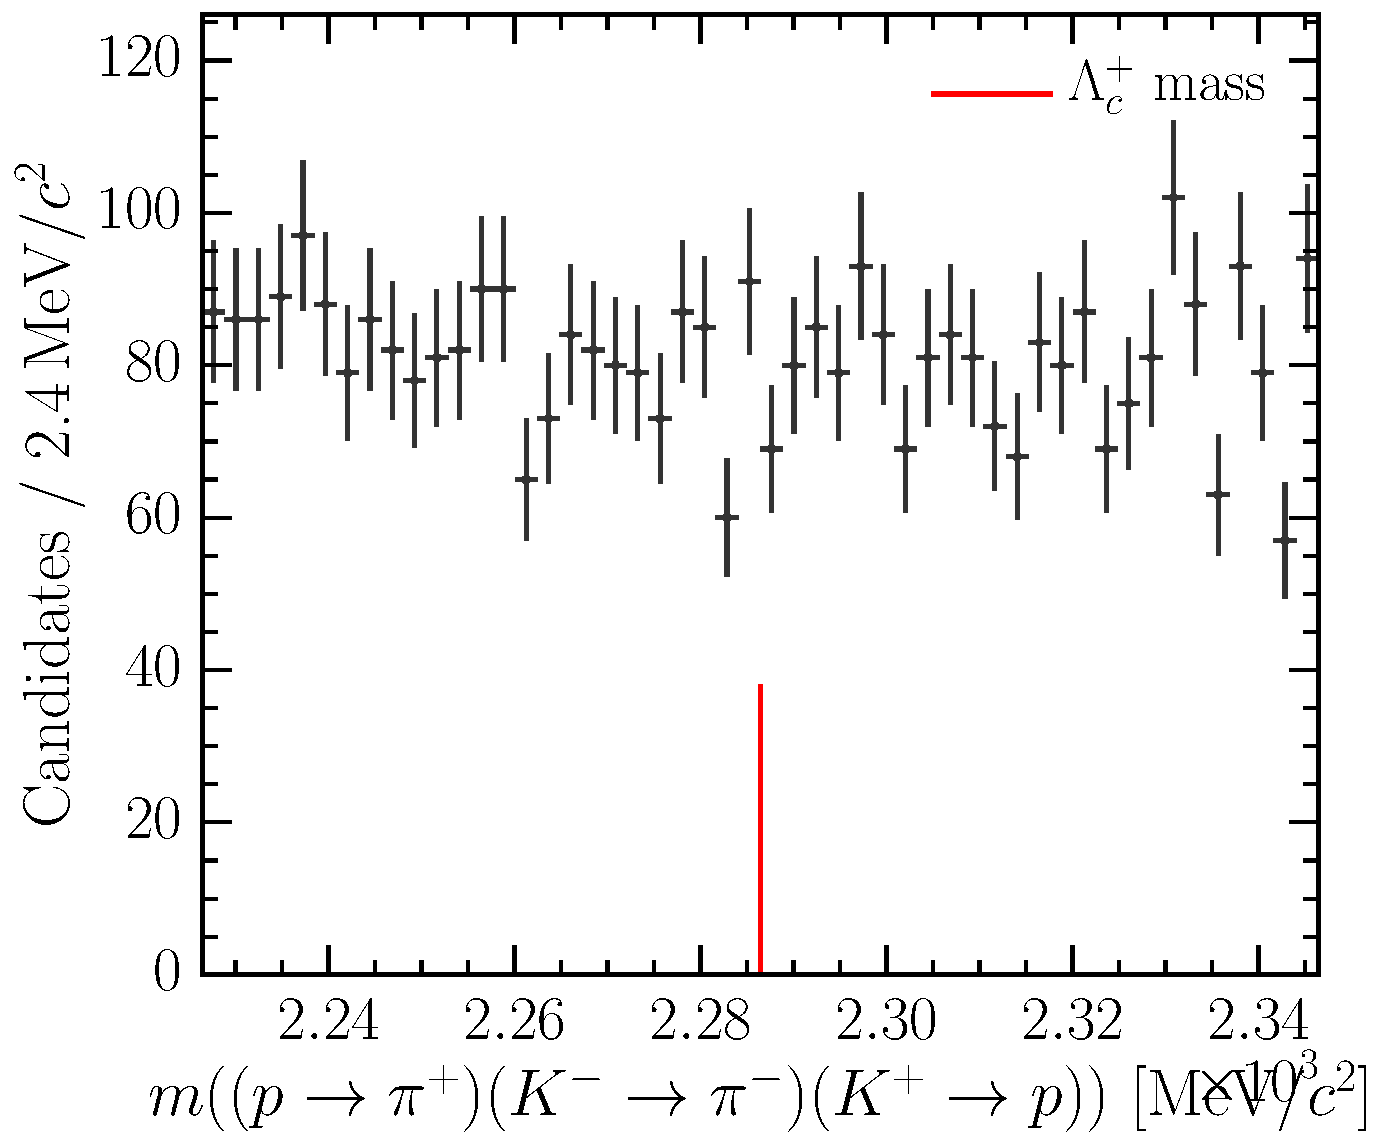
\includegraphics[width=\textwidth]{cpv/selection/background_study/pKK/LcTopKK_2012_MagDown_Lc_ppTopip_kmTopim_kpTopp}
    \caption{\decay{\PLambdac}{\Ppiplus\Ppiminus\Pproton}}
    \label{fig:cpv:selection:background_study:pKK_baryon:lcp_pipip}
  \end{subfigure}

  \begin{subfigure}[b]{0.3\textwidth}
    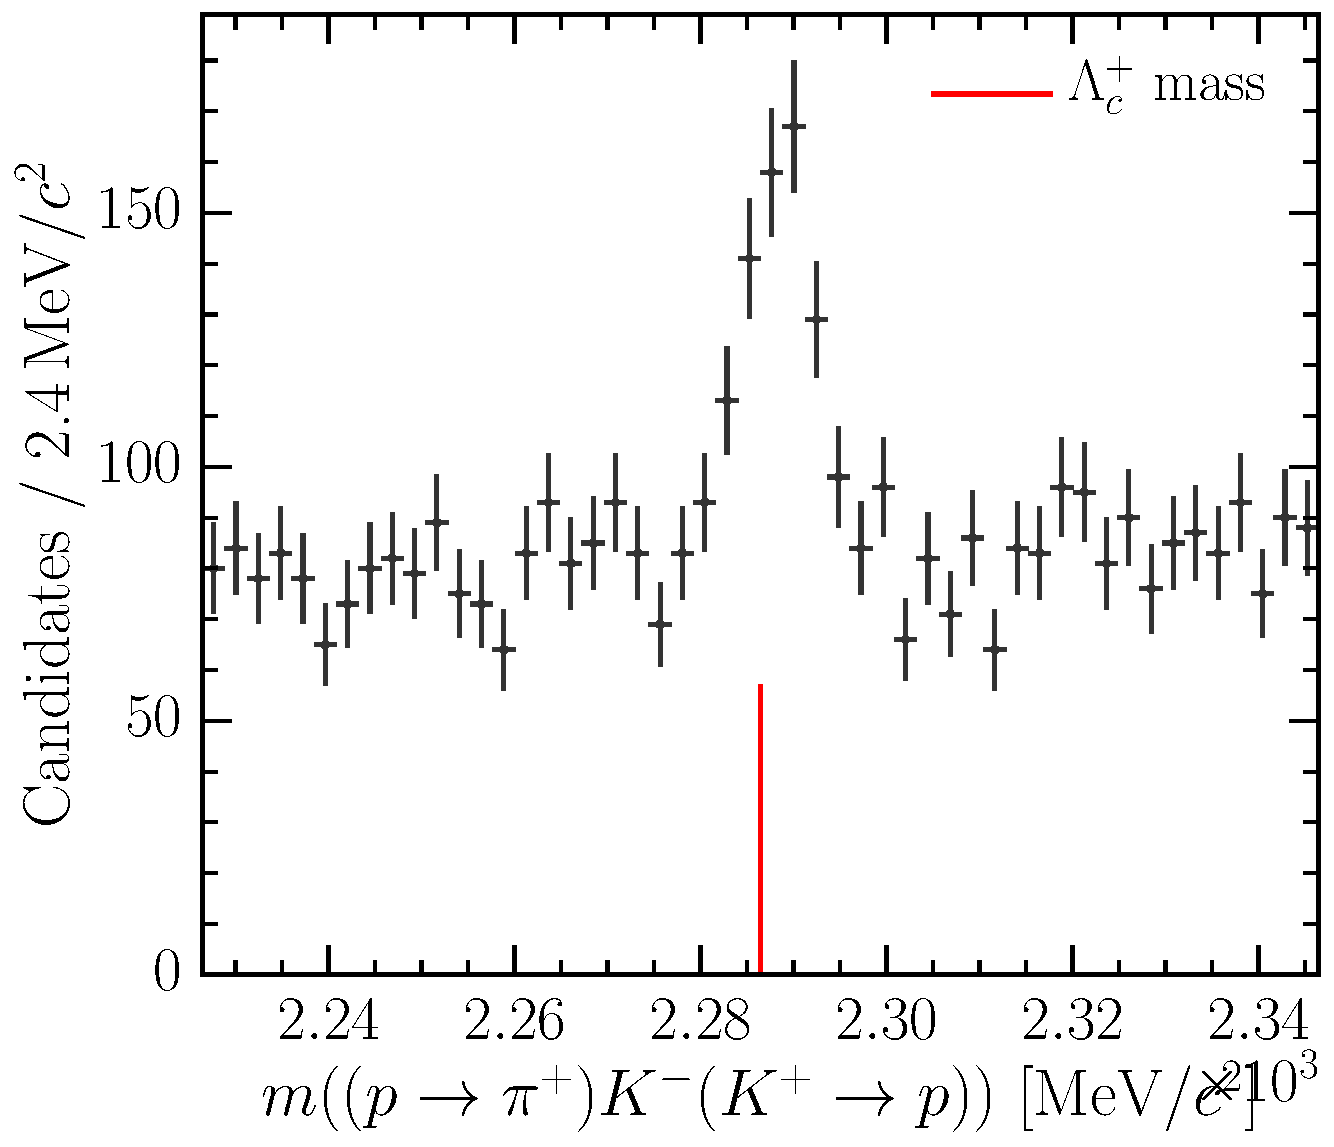
\includegraphics[width=\textwidth]{cpv/selection/background_study/pKK/LcTopKK_2012_MagDown_Lc_ppTopip_km_kpTopp}
    \caption{\decay{\PLambdac}{\Ppiplus\PKminus\Pproton}}
    \label{fig:cpv:selection:background_study:pKK_baryon:lcp_pikp}
  \end{subfigure}
  \begin{subfigure}[b]{0.3\textwidth}
    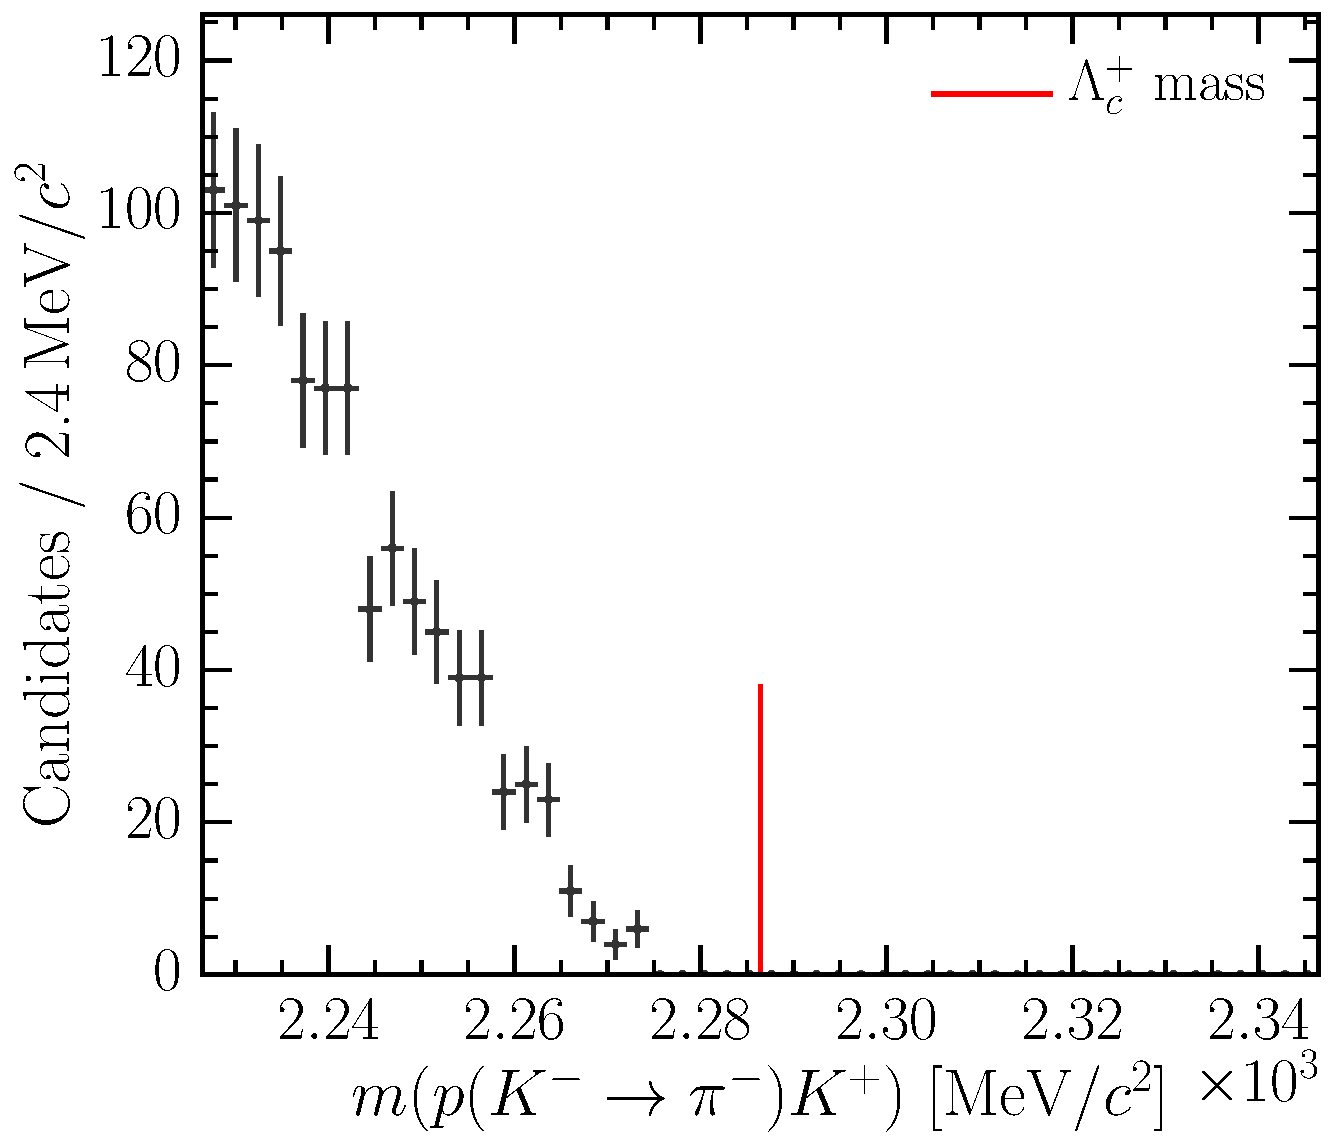
\includegraphics[width=\textwidth]{cpv/selection/background_study/pKK/LcTopKK_2012_MagDown_Lc_pp_kmTopim_kp}
    \caption{\decay{\PLambdac}{\Pproton\Ppiminus\PKplus}}
    \label{fig:cpv:selection:background_study:pKK_baryon:lcp_ppik}
  \end{subfigure}
  \begin{subfigure}[b]{0.3\textwidth}
    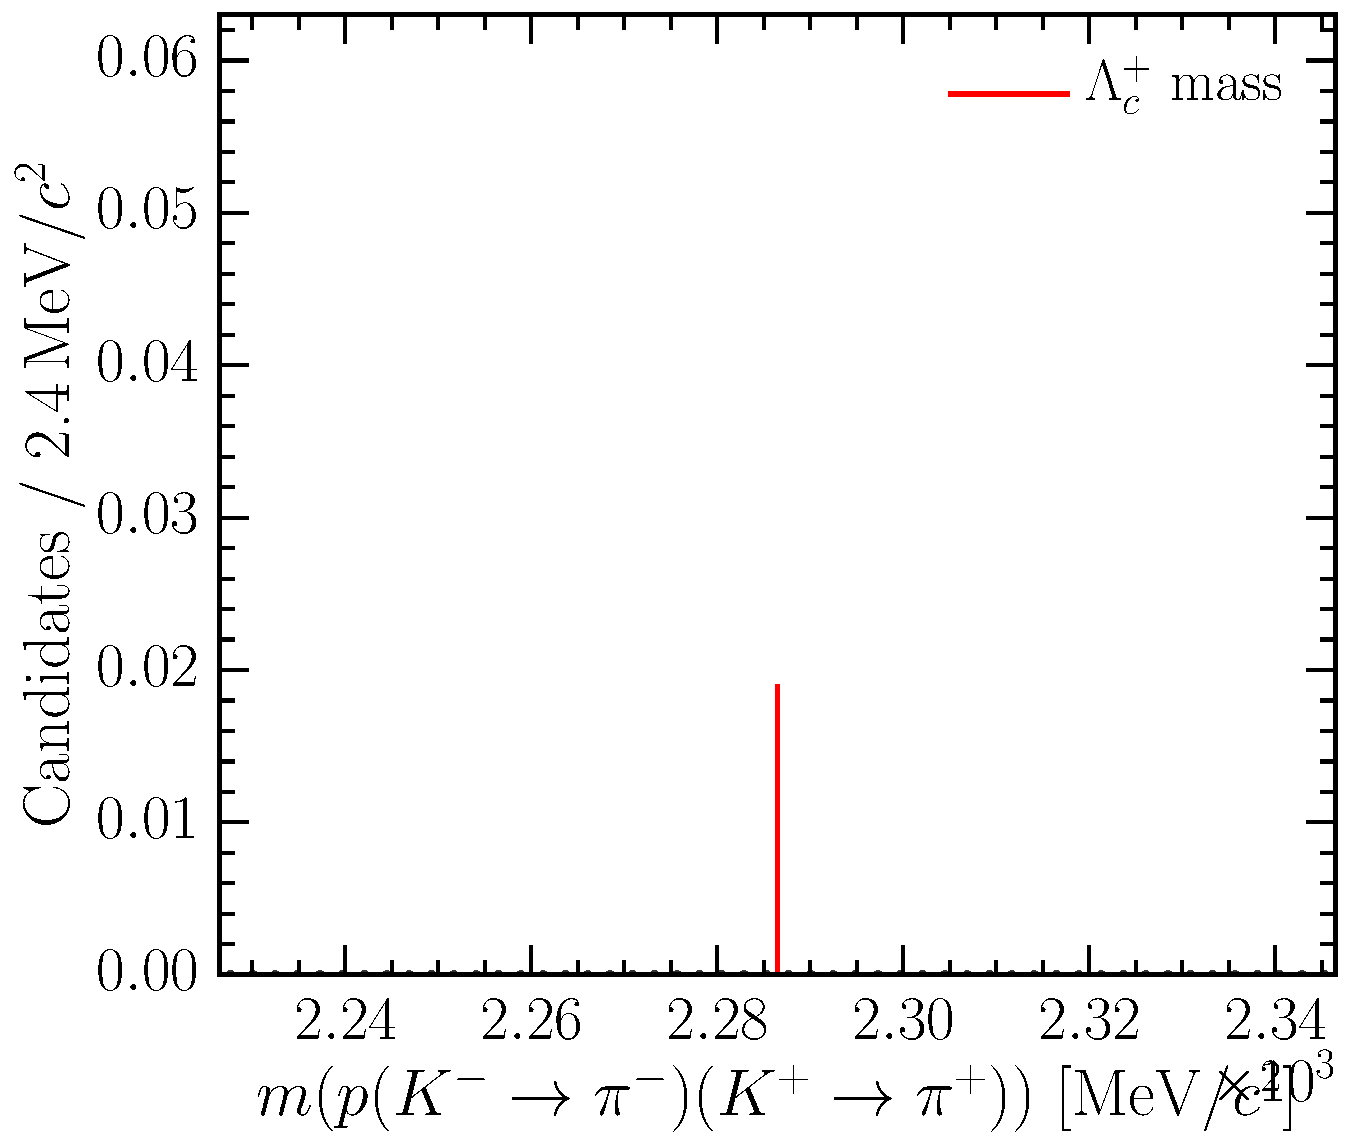
\includegraphics[width=\textwidth]{cpv/selection/background_study/pKK/LcTopKK_2012_MagDown_Lc_pp_kmTopim_kpTopip}
    \caption{\decay{\PLambdac}{\Pproton\Ppiminus\Ppiplus}}
    \label{fig:cpv:selection:background_study:pKK_baryon:lcp_ppipi}
  \end{subfigure}

  \begin{subfigure}[b]{0.3\textwidth}
    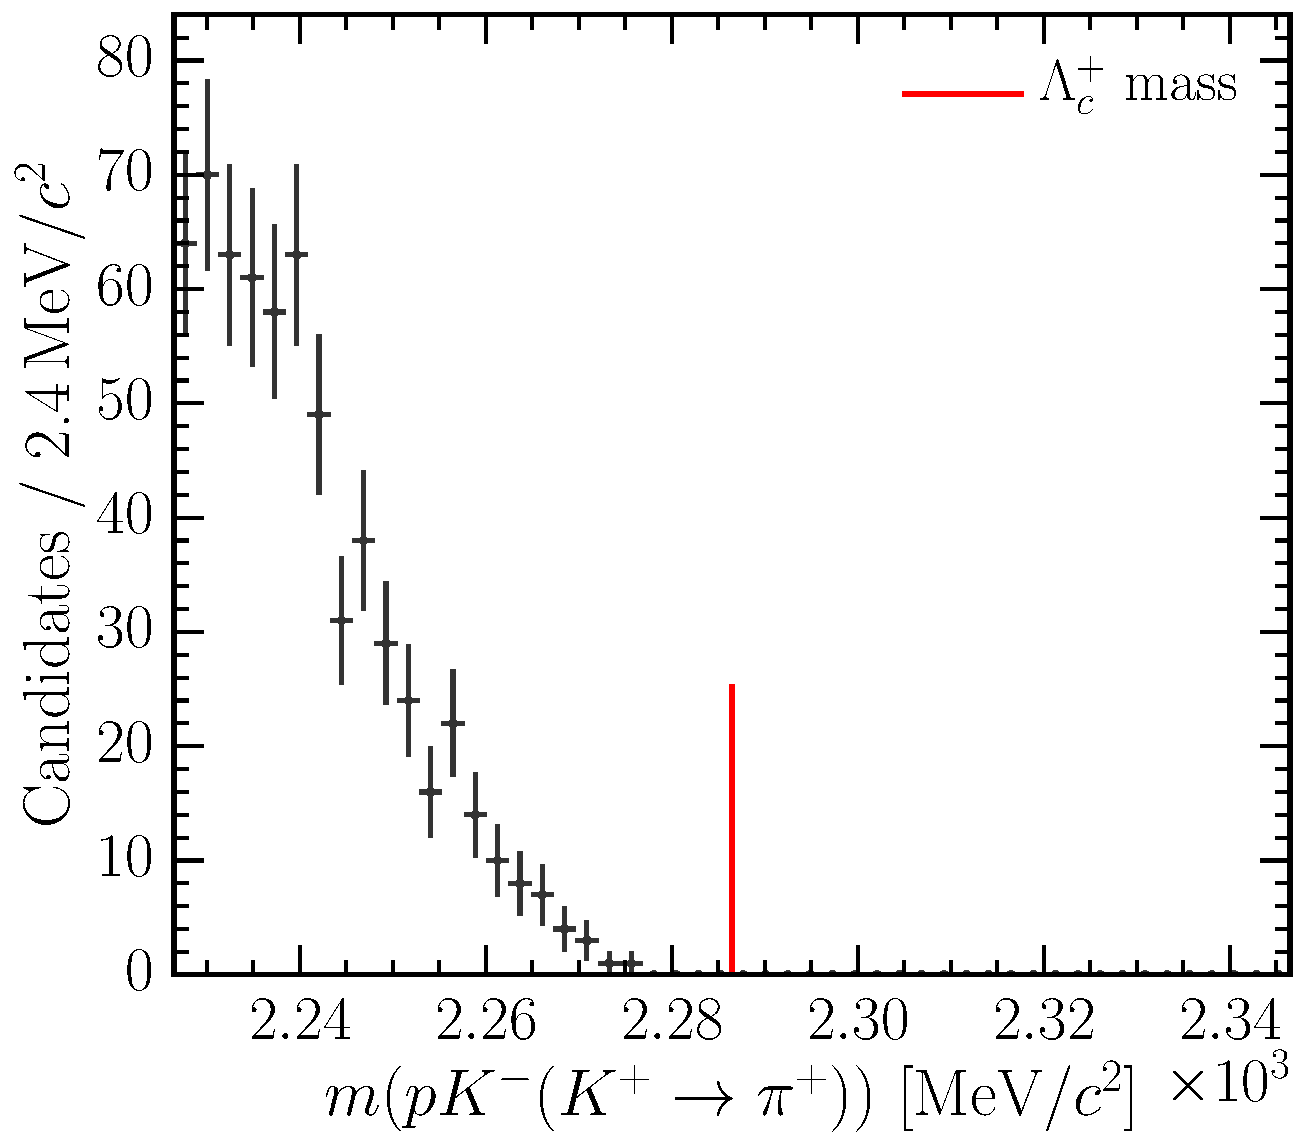
\includegraphics[width=\textwidth]{cpv/selection/background_study/pKK/LcTopKK_2012_MagDown_Lc_pp_km_kpTopip}
    \caption{\decay{\PLambdac}{\Pproton\PKminus\Ppiplus}}
    \label{fig:cpv:selection:background_study:pKK_baryon:lcp_pkpi}
  \end{subfigure}

  \caption{%
    Wrong-mass distributions obtained when changing the mass hypotheses of the
    fully selected \PLambdac\ children in the \pKK\ mode, where one child is
    assigned the proton mass hypothesis.
    The $x$-axis on each sub-figure shows the substitutions that have been
    made.
    For example, the ${\Pproton\PKminus(\PKplus \to \Ppiplus)}$ distribution is where the
    nominal kaon with same charge as the proton has been also assigned the pion
    hypothesis.
    The vertical red lines indicate the nominal mass of the misidentified 
    particle under study.
    Only the 2012 magnet down data is shown.
  }
  \label{fig:cpv:selection:background_study:pKK_baryon}
\end{figure}

\begin{figure}
  \centering
  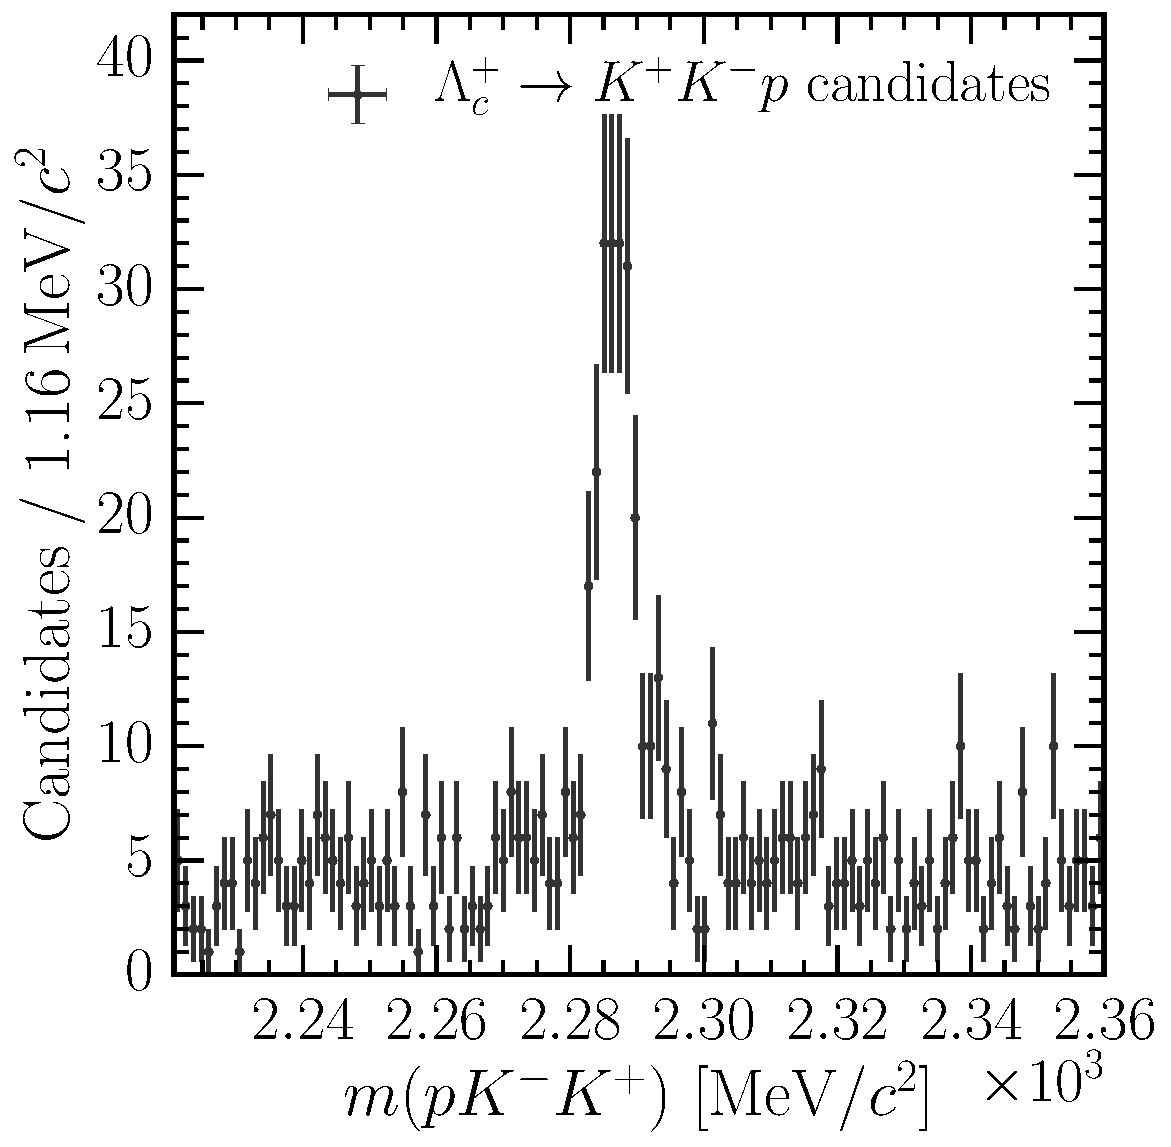
\includegraphics[width=0.5\textwidth]{cpv/selection/background_study/pKK/LcTopKK_2012_MagDown_Lc_ppTokp_km_kpTopp-Lc_M}
  \caption{%
    Mass spectrum of \pKK\ candidates that fall within \SI{8}{\MeV} of the
    nominal \PLambdac\ mass when the proton and same-sign kaon mass hypotheses
    are swapped.
    The mass spectrum of \PLambdac\ candidates with the swapped hypotheses is
    shown in
    Figure~\ref{fig:cpv:selection:background_study:pKK_baryon:lcp_KKp}.
    The lack of structures other than the flat combinatorial-background-like
    and peaking signal-like components indicate that the presence of this
    misidentification background does not affect the nominal \pKK\ yield
    extraction.
  }
  \label{fig:cpv:selection:background_study:pKK_lcp_KKp_Lc_M}
\end{figure}

\begin{figure}
  \begin{subfigure}[b]{0.3\textwidth}
    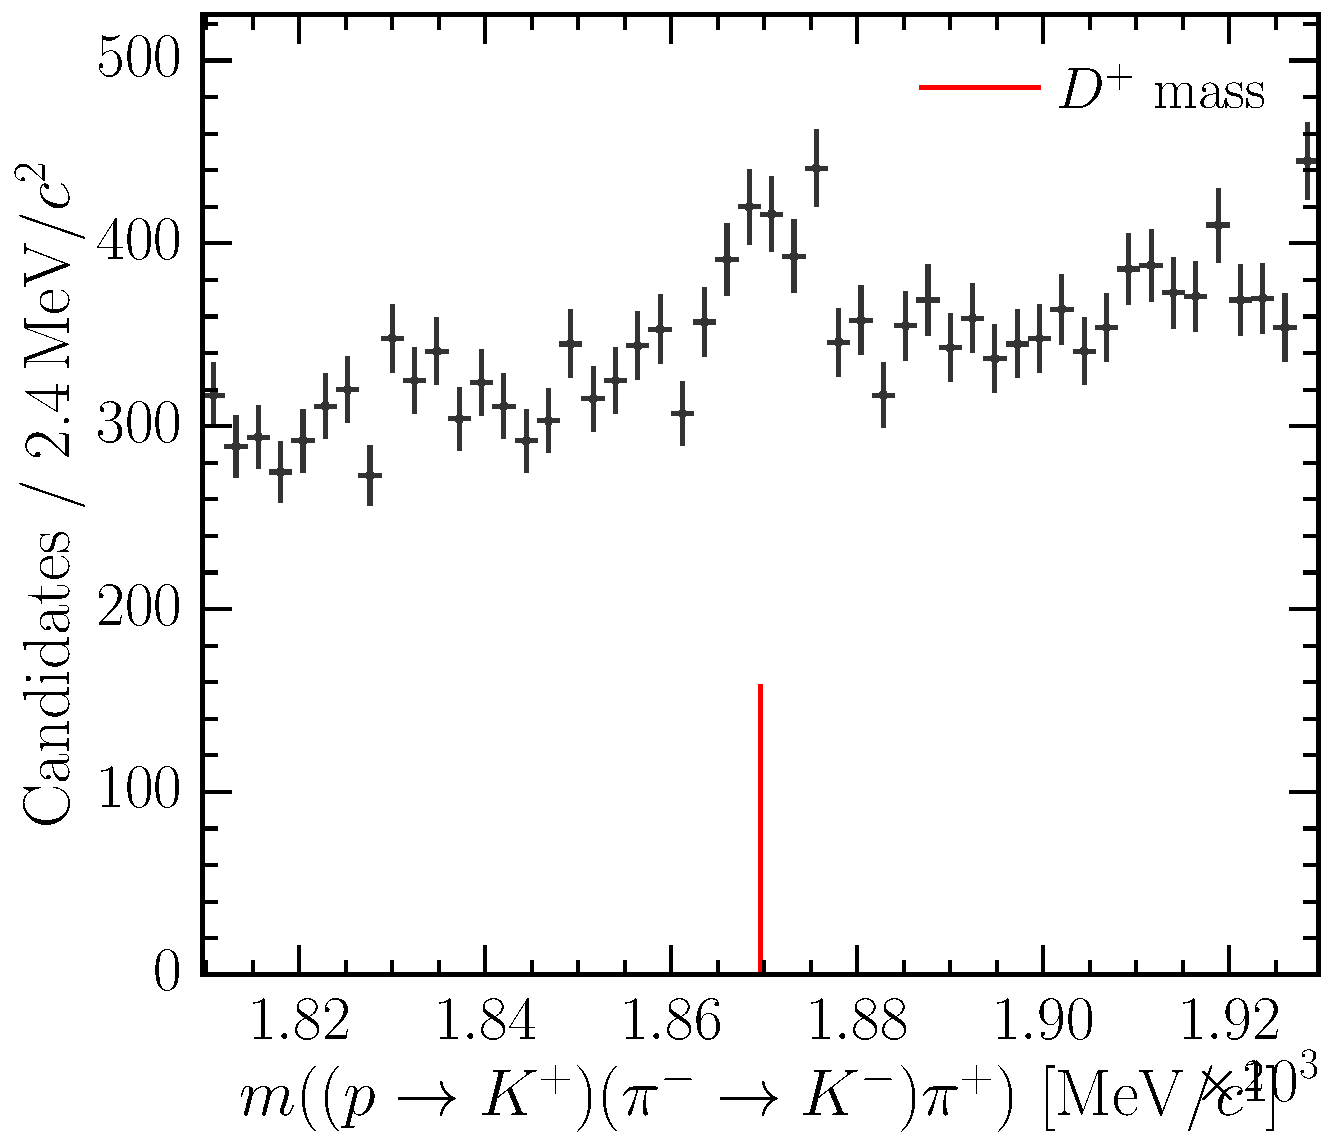
\includegraphics[width=\textwidth]{figures/cpv/selection/background_study/ppipi/LcToppipi_2012_MagDown_Dp_ppTokp_pimTokm_pip}
    \caption{\decay{\PDplus}{\PKplus\PKminus\Ppiplus}}
    \label{fig:cpv:selection:background_study:ppipi_meson:dplus_kkpi}
  \end{subfigure}
  \begin{subfigure}[b]{0.3\textwidth}
    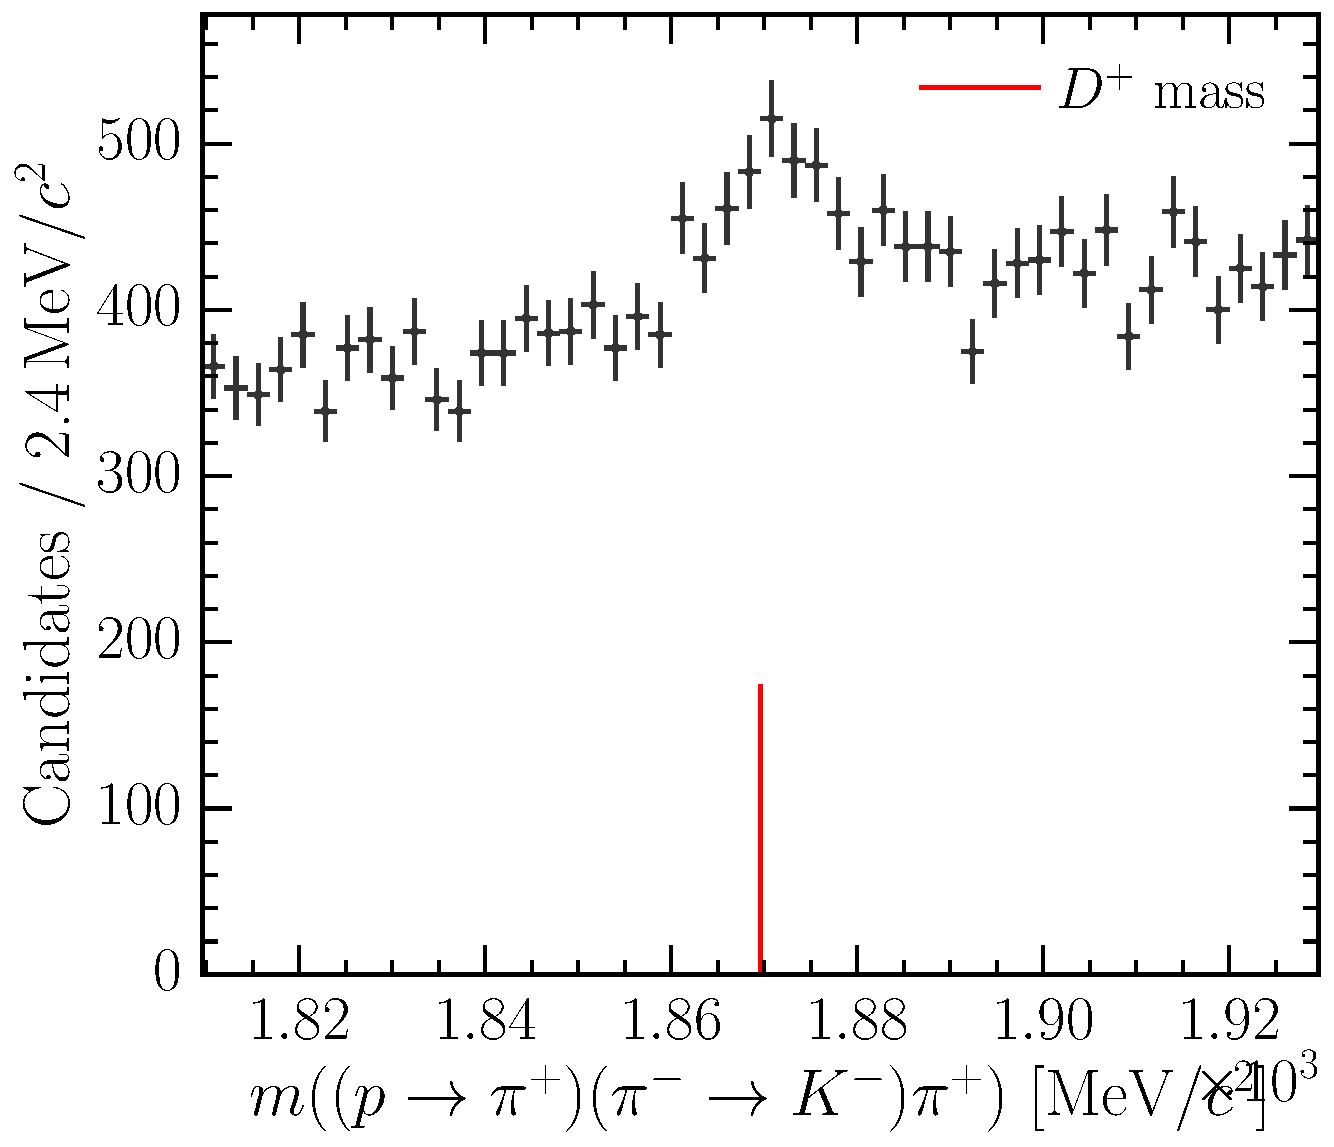
\includegraphics[width=\textwidth]{figures/cpv/selection/background_study/ppipi/LcToppipi_2012_MagDown_Dp_ppTopip_pimTokm_pip}
    \caption{\decay{\PDplus}{\Ppiplus\PKminus\Ppiplus}}
    \label{fig:cpv:selection:background_study:ppipi_meson:dplus_pikpi}
  \end{subfigure}
  \begin{subfigure}[b]{0.3\textwidth}
    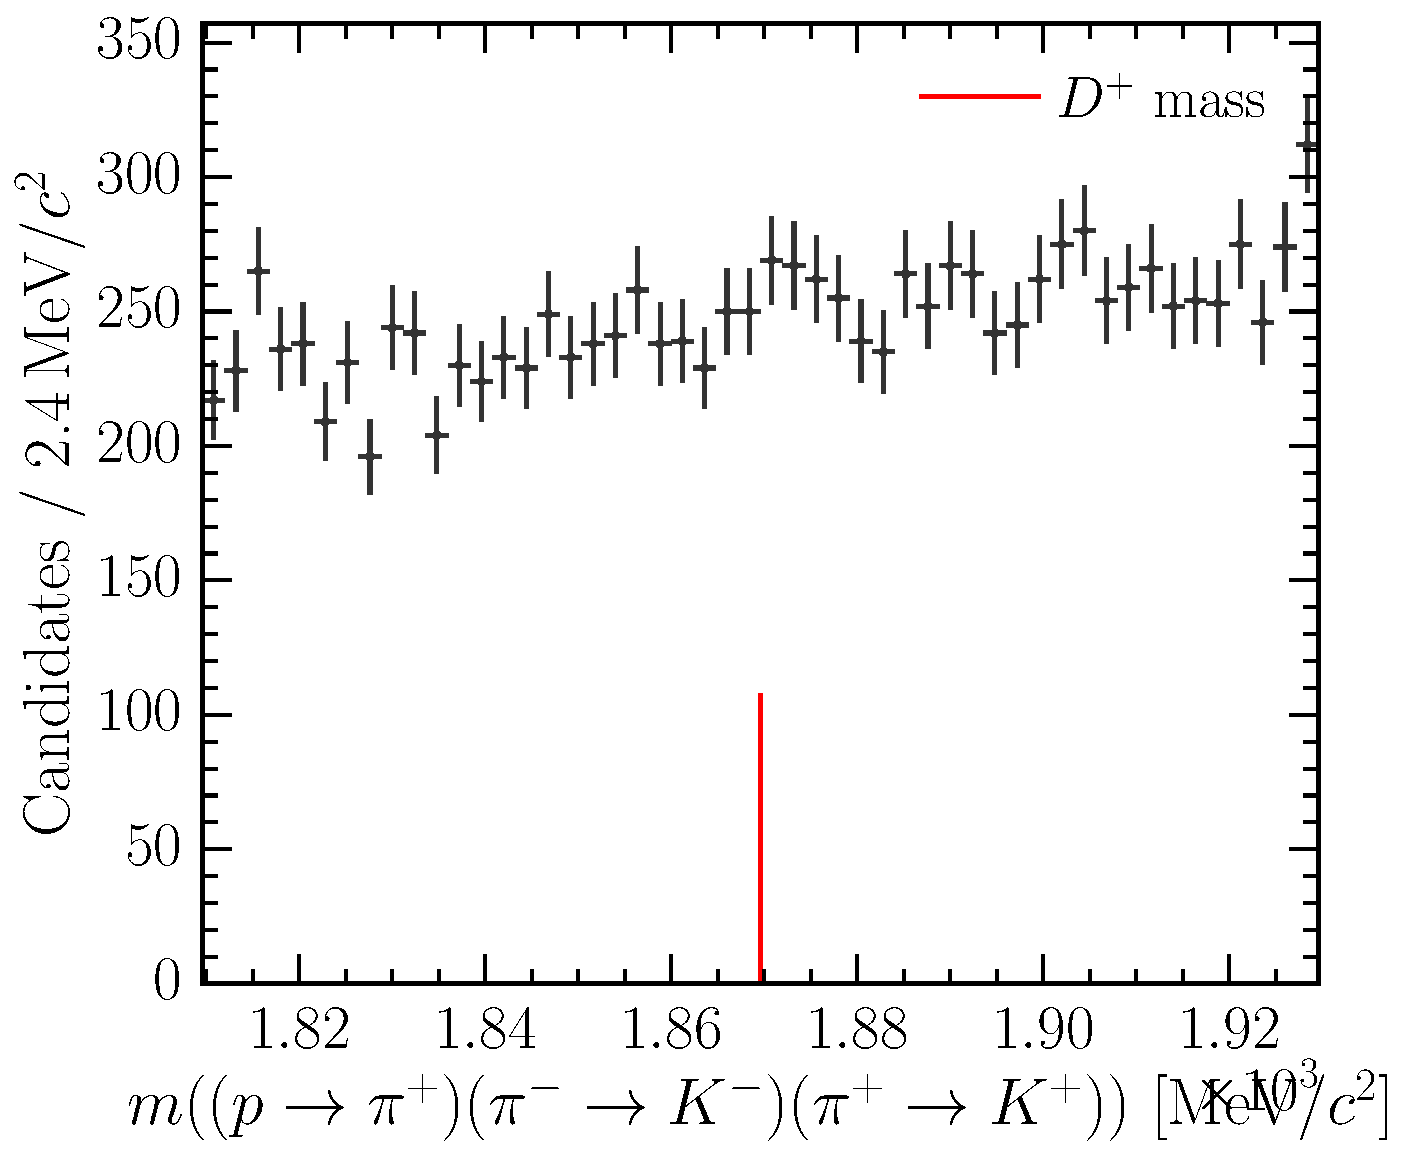
\includegraphics[width=\textwidth]{figures/cpv/selection/background_study/ppipi/LcToppipi_2012_MagDown_Dp_ppTopip_pimTokm_pipTokp}
    \caption{\decay{\PDplus}{\Ppiplus\PKminus\PKplus}}
    \label{fig:cpv:selection:background_study:ppipi_meson:dplus_pikk}
  \end{subfigure}
  \begin{subfigure}[b]{0.3\textwidth}
    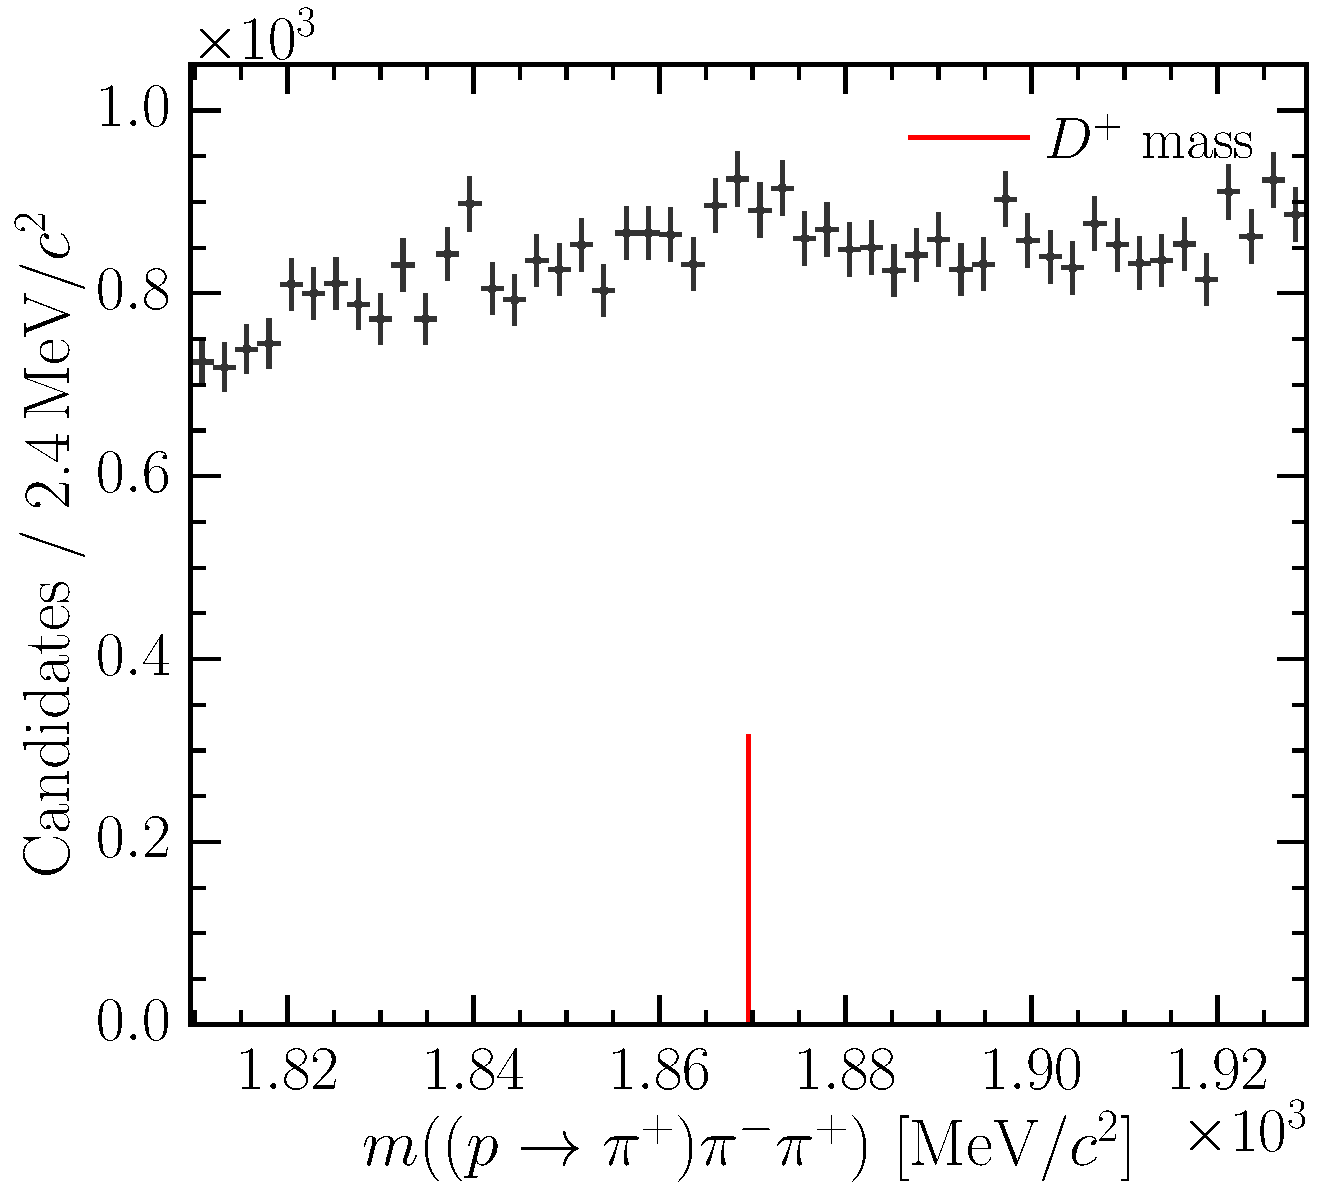
\includegraphics[width=\textwidth]{figures/cpv/selection/background_study/ppipi/LcToppipi_2012_MagDown_Dp_ppTopip_pim_pip}
    \caption{\decay{\PDplus}{\Ppiplus\Ppiminus\Ppiplus}}
    \label{fig:cpv:selection:background_study:ppipi_meson:dplus_pipipi}
  \end{subfigure}
  \begin{subfigure}[b]{0.3\textwidth}
    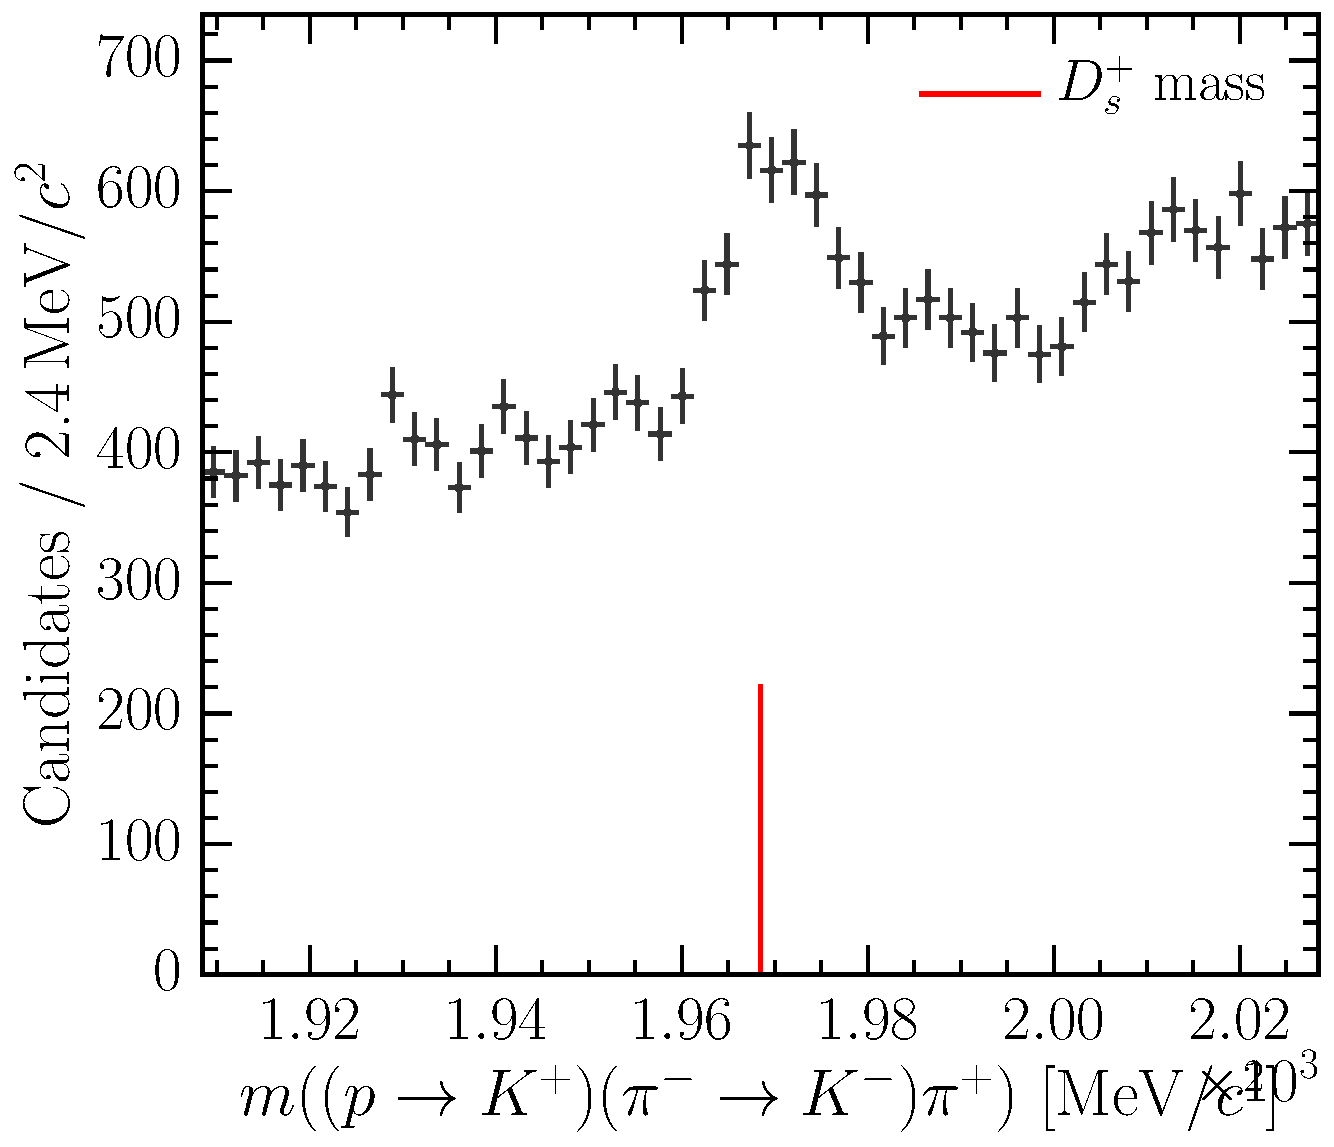
\includegraphics[width=\textwidth]{figures/cpv/selection/background_study/ppipi/LcToppipi_2012_MagDown_Ds_ppTokp_pimTokm_pip}
    \caption{\decay{\PDsplus}{\PKplus\PKminus\Ppiplus}}
    \label{fig:cpv:selection:background_study:ppipi_meson:dsplus_kkpi}
  \end{subfigure}
  \begin{subfigure}[b]{0.3\textwidth}
    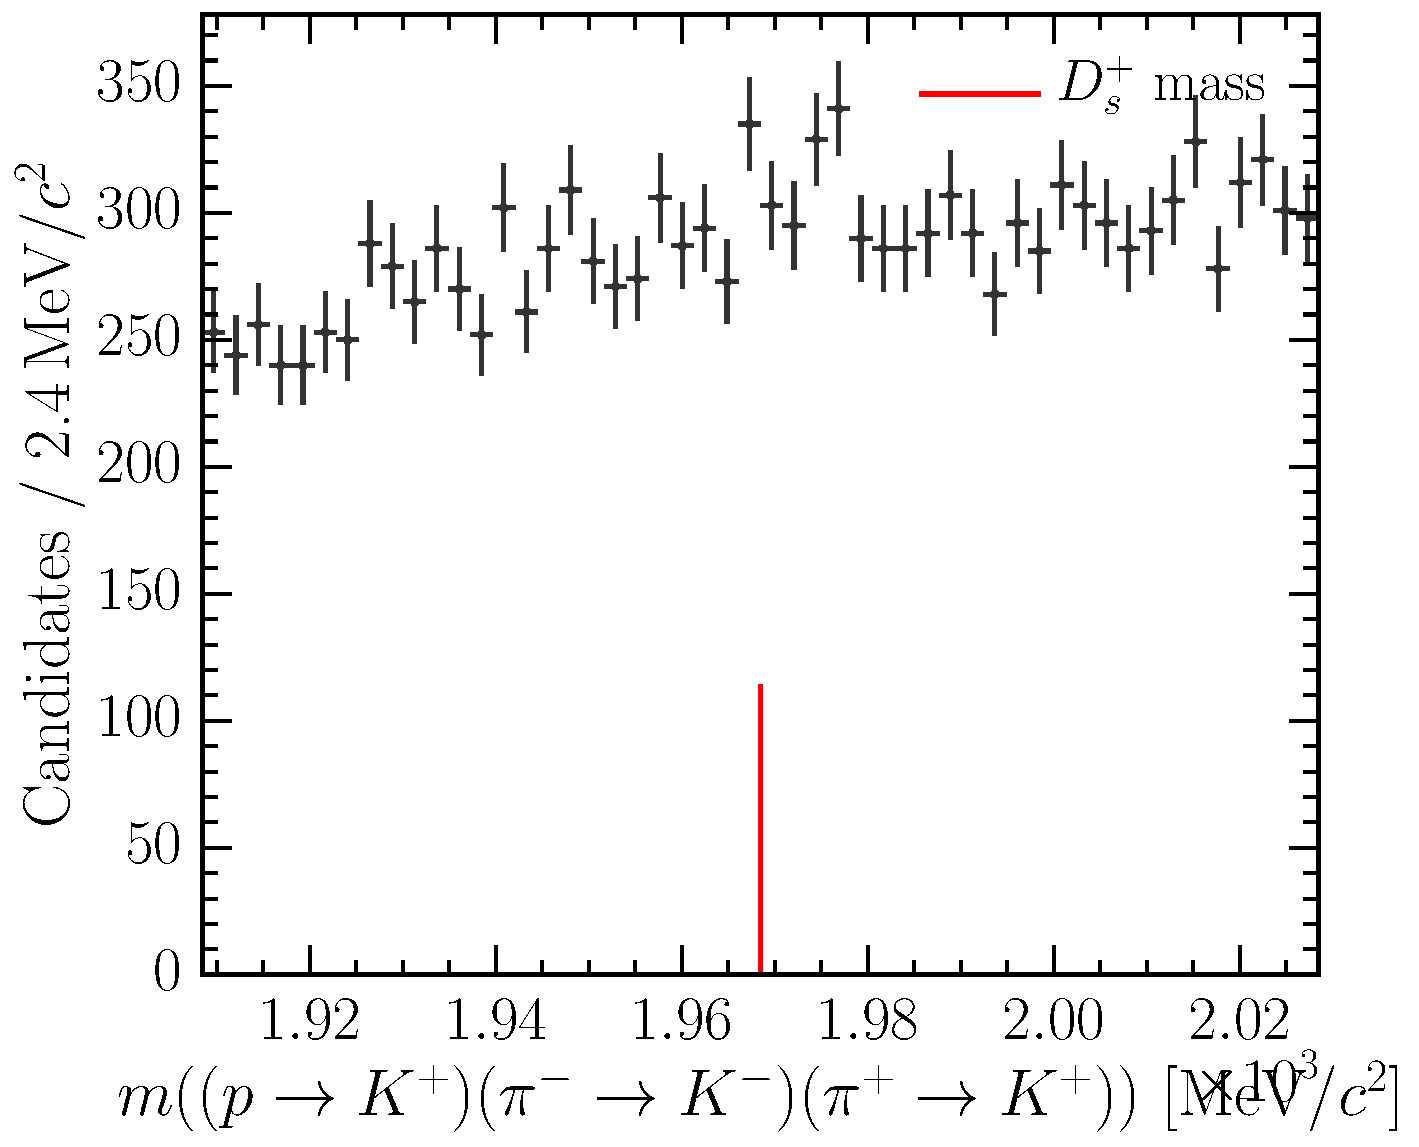
\includegraphics[width=\textwidth]{figures/cpv/selection/background_study/ppipi/LcToppipi_2012_MagDown_Ds_ppTokp_pimTokm_pipTokp}
    \caption{\decay{\PDsplus}{\PKplus\PKminus\PKplus}}
    \label{fig:cpv:selection:background_study:ppipi_meson:dsplus_kkk}
  \end{subfigure}
  \begin{subfigure}[b]{0.3\textwidth}
    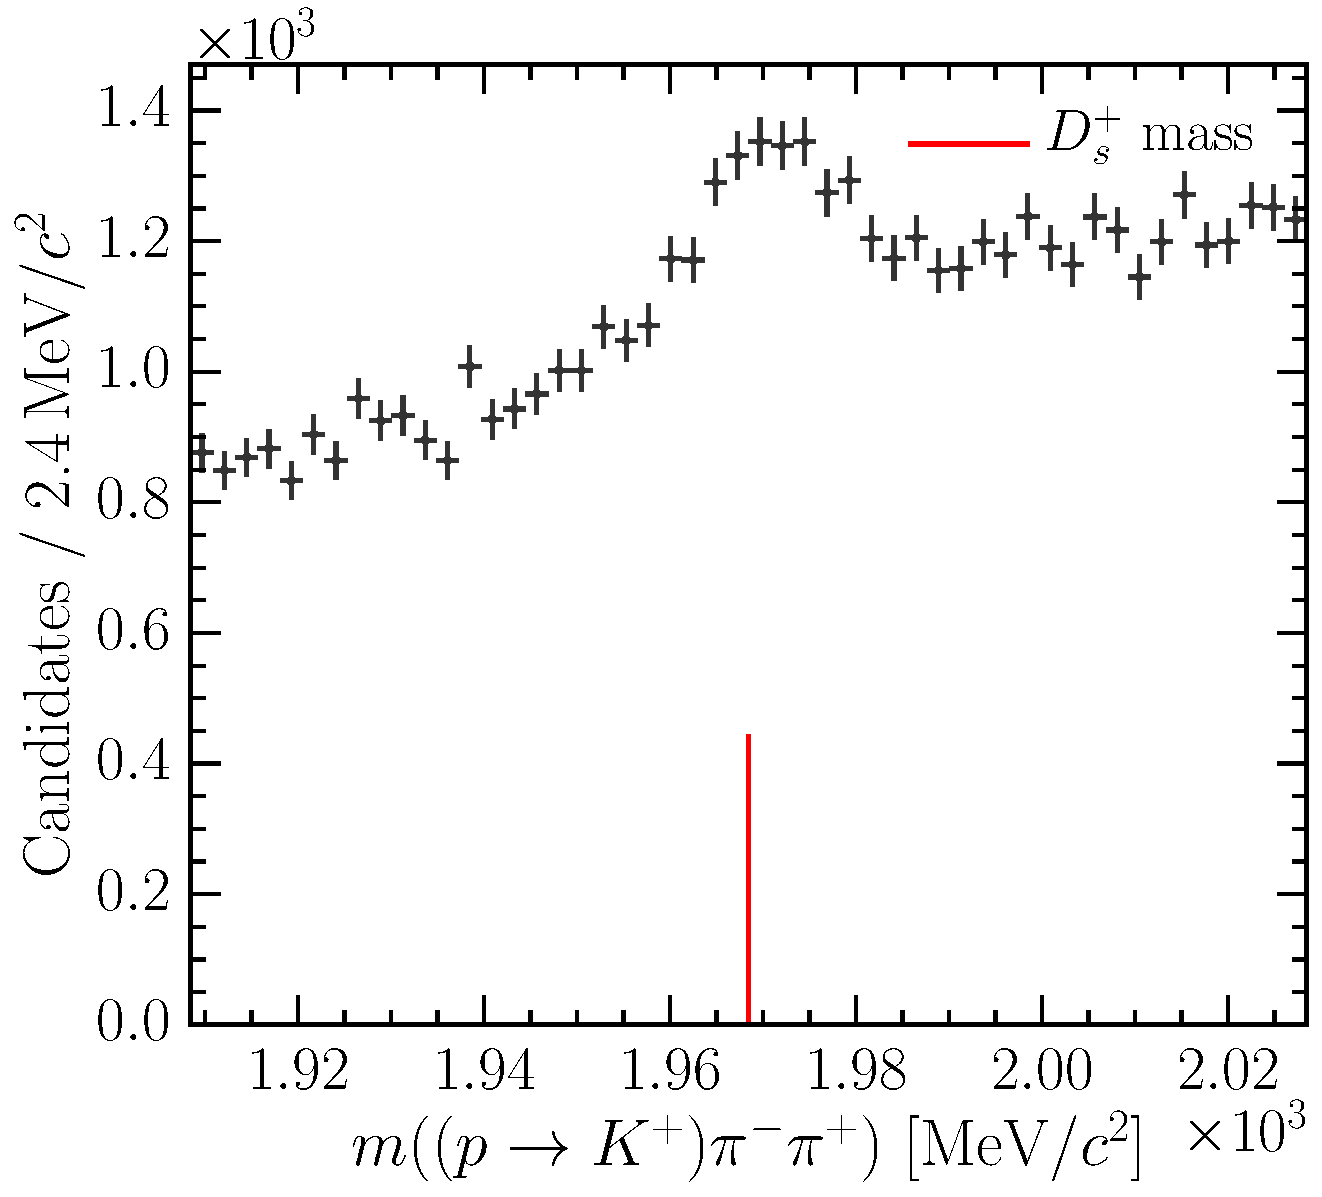
\includegraphics[width=\textwidth]{figures/cpv/selection/background_study/ppipi/LcToppipi_2012_MagDown_Ds_ppTokp_pim_pip}
    \caption{\decay{\PDsplus}{\PKplus\Ppiminus\Ppiplus}}
    \label{fig:cpv:selection:background_study:ppipi_meson:dsplus_kpipi}
  \end{subfigure}
  \begin{subfigure}[b]{0.3\textwidth}
    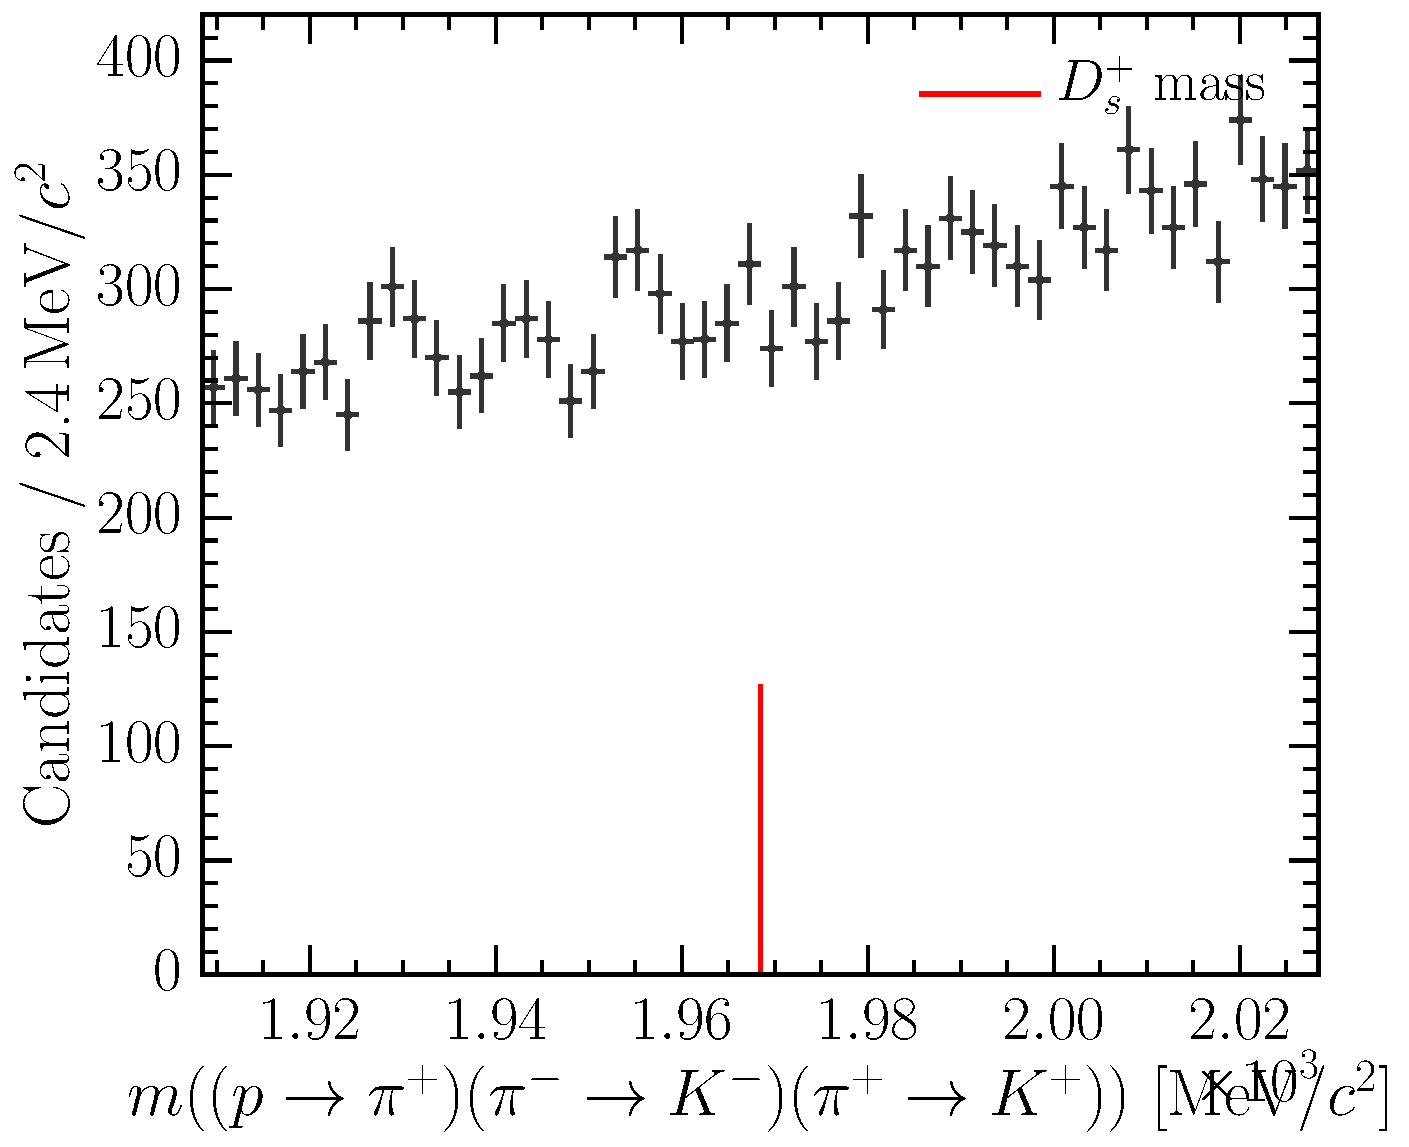
\includegraphics[width=\textwidth]{figures/cpv/selection/background_study/ppipi/LcToppipi_2012_MagDown_Ds_ppTopip_pimTokm_pipTokp}
    \caption{\decay{\PDsplus}{\Ppiplus\PKminus\PKplus}}
    \label{fig:cpv:selection:background_study:ppipi_meson:dsplus_pikk}
  \end{subfigure}
  \begin{subfigure}[b]{0.3\textwidth}
    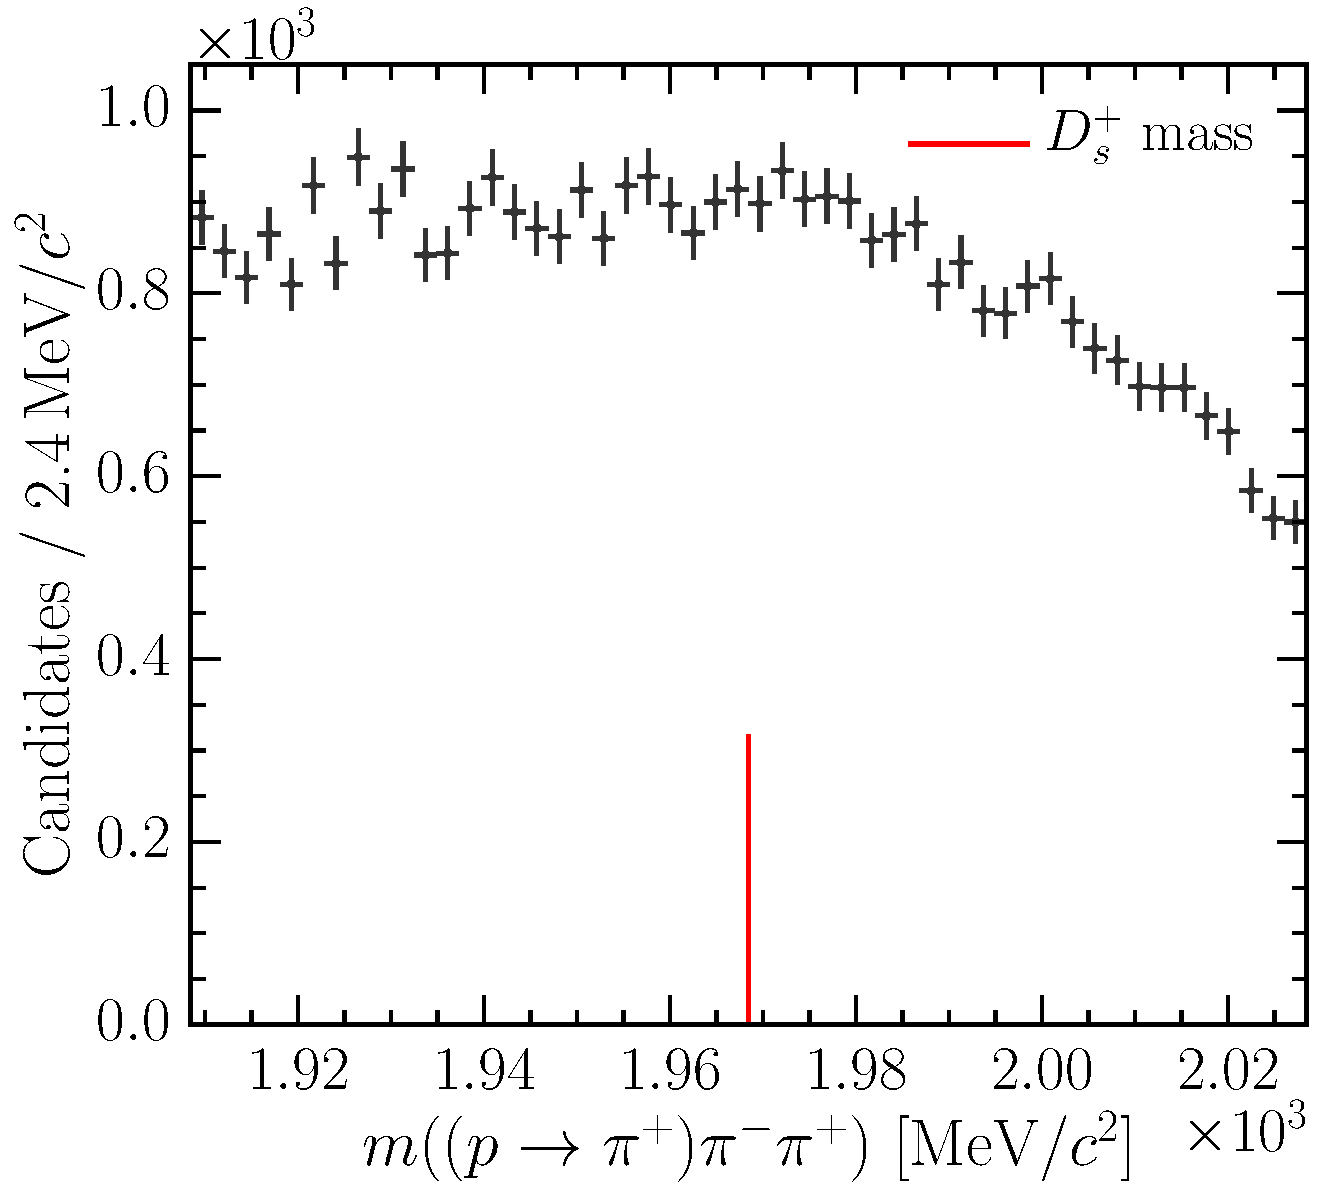
\includegraphics[width=\textwidth]{figures/cpv/selection/background_study/ppipi/LcToppipi_2012_MagDown_Ds_ppTopip_pim_pip}
    \caption{\decay{\PDsplus}{\Ppiplus\Ppiminus\Ppiplus}}
    \label{fig:cpv:selection:background_study:ppipi_meson:dsplus_pipipi}
  \end{subfigure}
  \begin{subfigure}[b]{0.3\textwidth}
    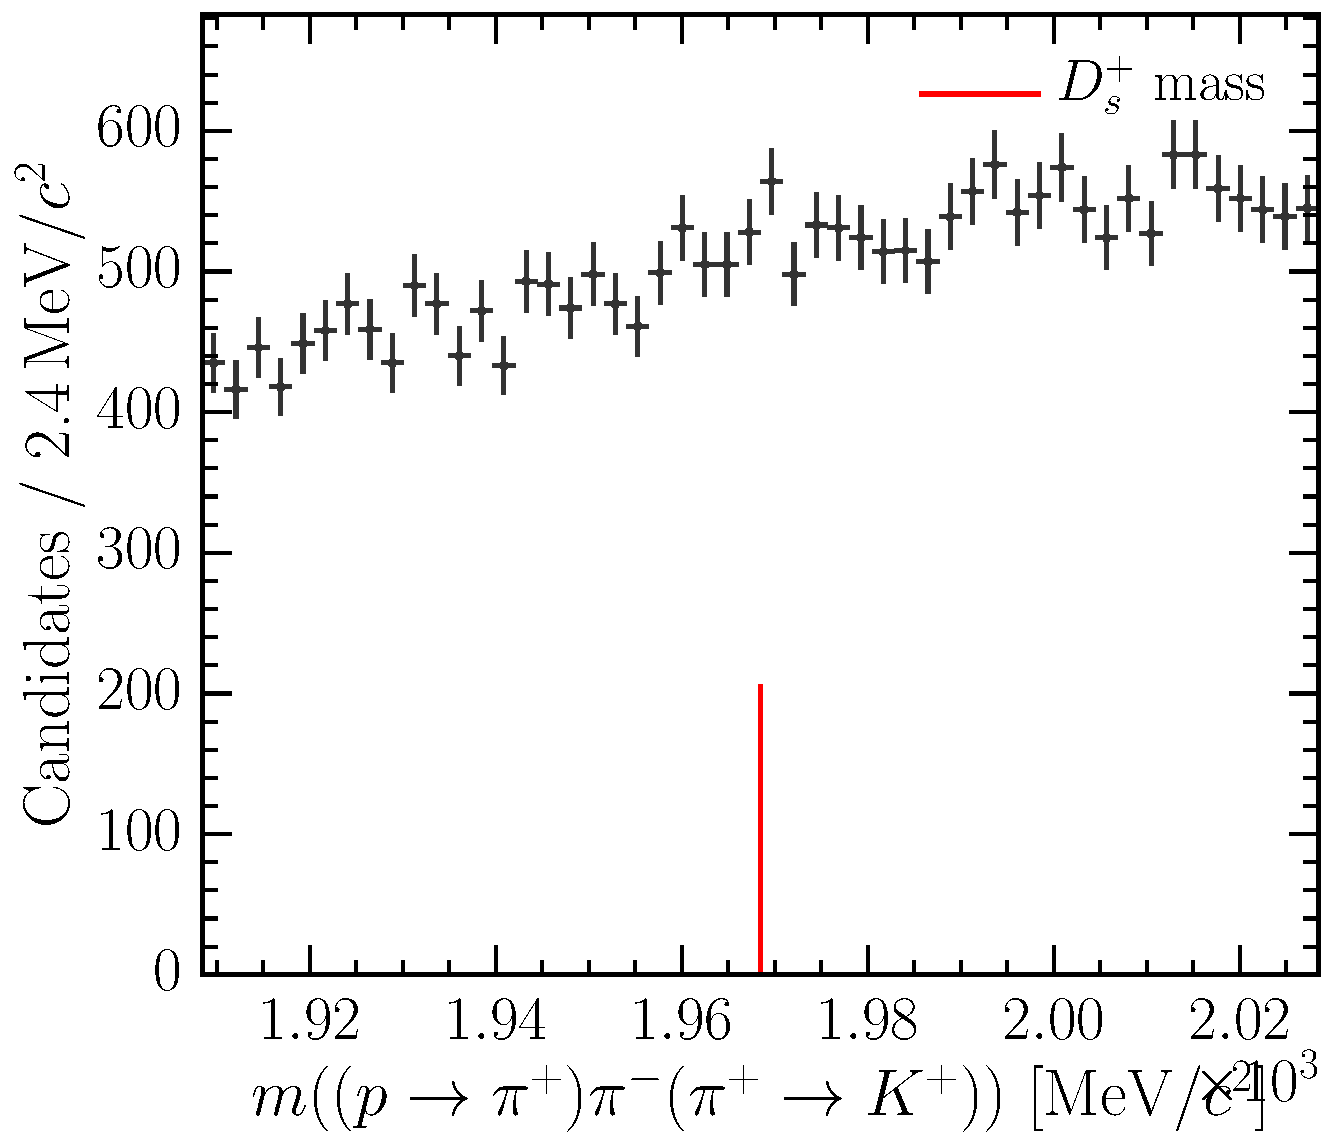
\includegraphics[width=\textwidth]{figures/cpv/selection/background_study/ppipi/LcToppipi_2012_MagDown_Ds_ppTopip_pim_pipTokp}
    \caption{\decay{\PDsplus}{\Ppiplus\Ppiminus\PKplus}}
    \label{fig:cpv:selection:background_study:ppipi_meson:dsplus_pipik}
  \end{subfigure}
  \caption{%
    Wrong-mass distributions obtained when changing the mass hypotheses of the
    fully selected \PLambdac\ children in the \ppipi\ mode, where no child is
    assigned the proton mass hypothesis.
    The $x$-axis on each sub-figure shows the substitutions that have been
    made.
    For example, the ${(\Pproton \to \Ppiplus)(\Ppiminus \to \PKminus)\Ppiplus}$ distribution is
    where the nominal proton candidate has been assigned the pion mass
    hypothesis, and the nominal pion with opposite charge to the proton has
    been assigned the kaon hypothesis.
    The vertical red lines indicate the nominal mass of the misidentified 
    particle under study.
    Only the 2012 magnet down data is shown.
  }
  \label{fig:cpv:selection:background_study:ppipi_meson}
\end{figure}

\begin{figure}
  \begin{subfigure}[b]{0.3\textwidth}
    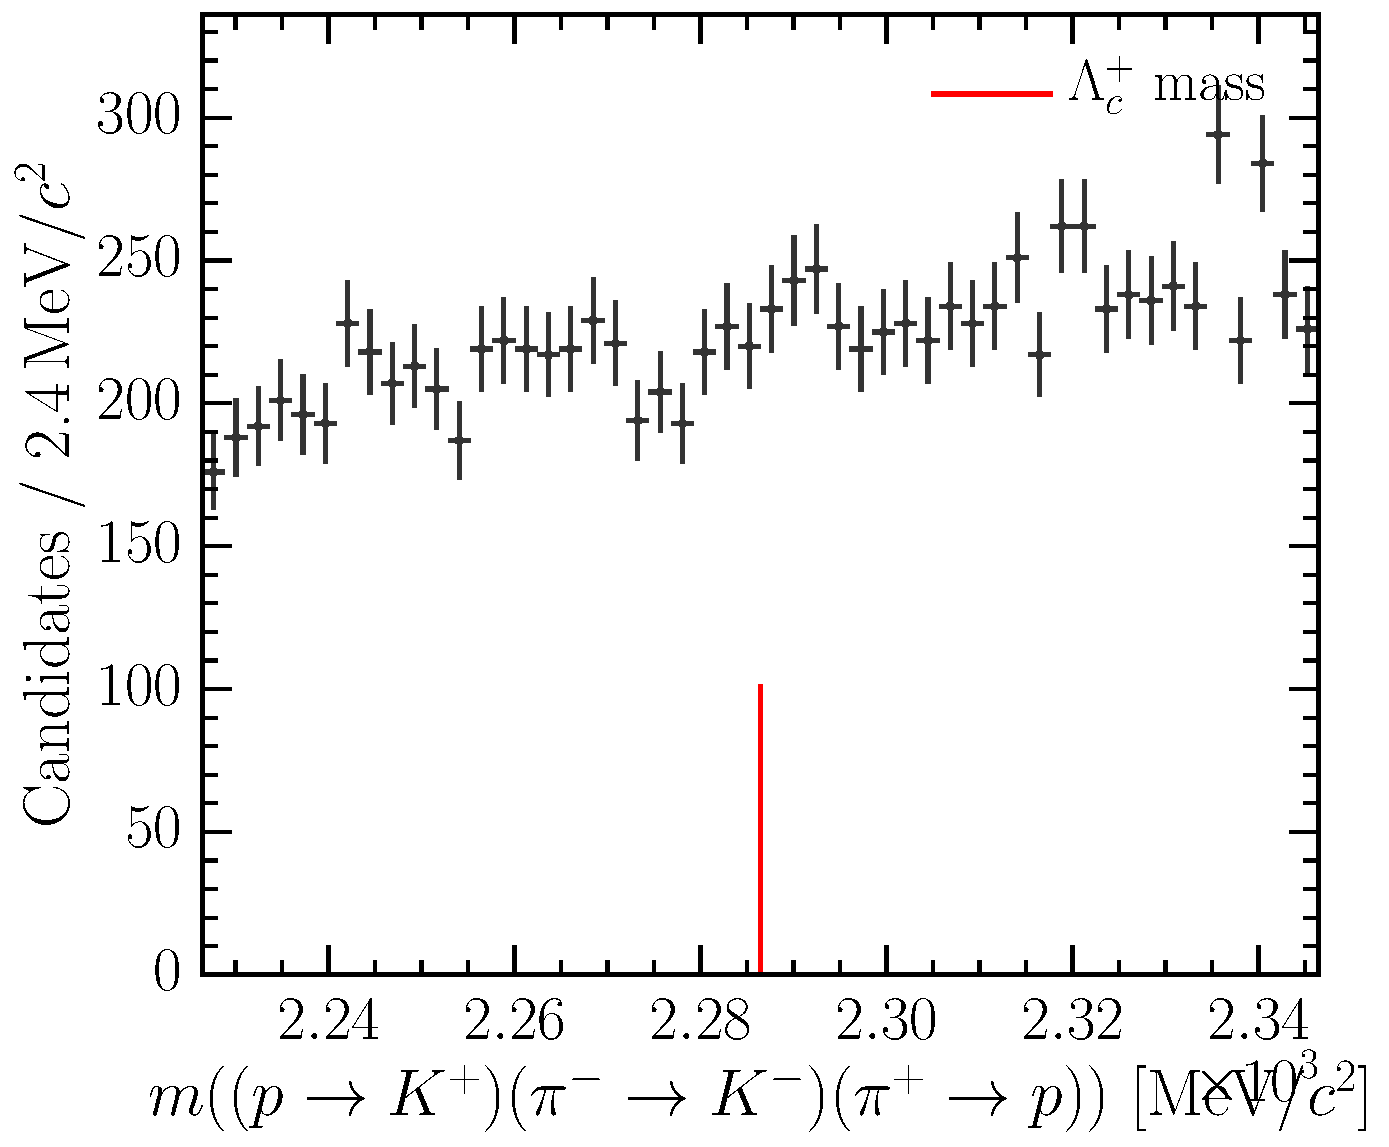
\includegraphics[width=\textwidth]{figures/cpv/selection/background_study/ppipi/LcToppipi_2012_MagDown_Lc_ppTokp_pimTokm_pipTopp}
    \caption{\decay{\PLambdac}{\PKplus\PKminus\Pproton}}
    \label{fig:cpv:selection:background_study:ppipi_baryon:kkp}
  \end{subfigure}
  \begin{subfigure}[b]{0.3\textwidth}
    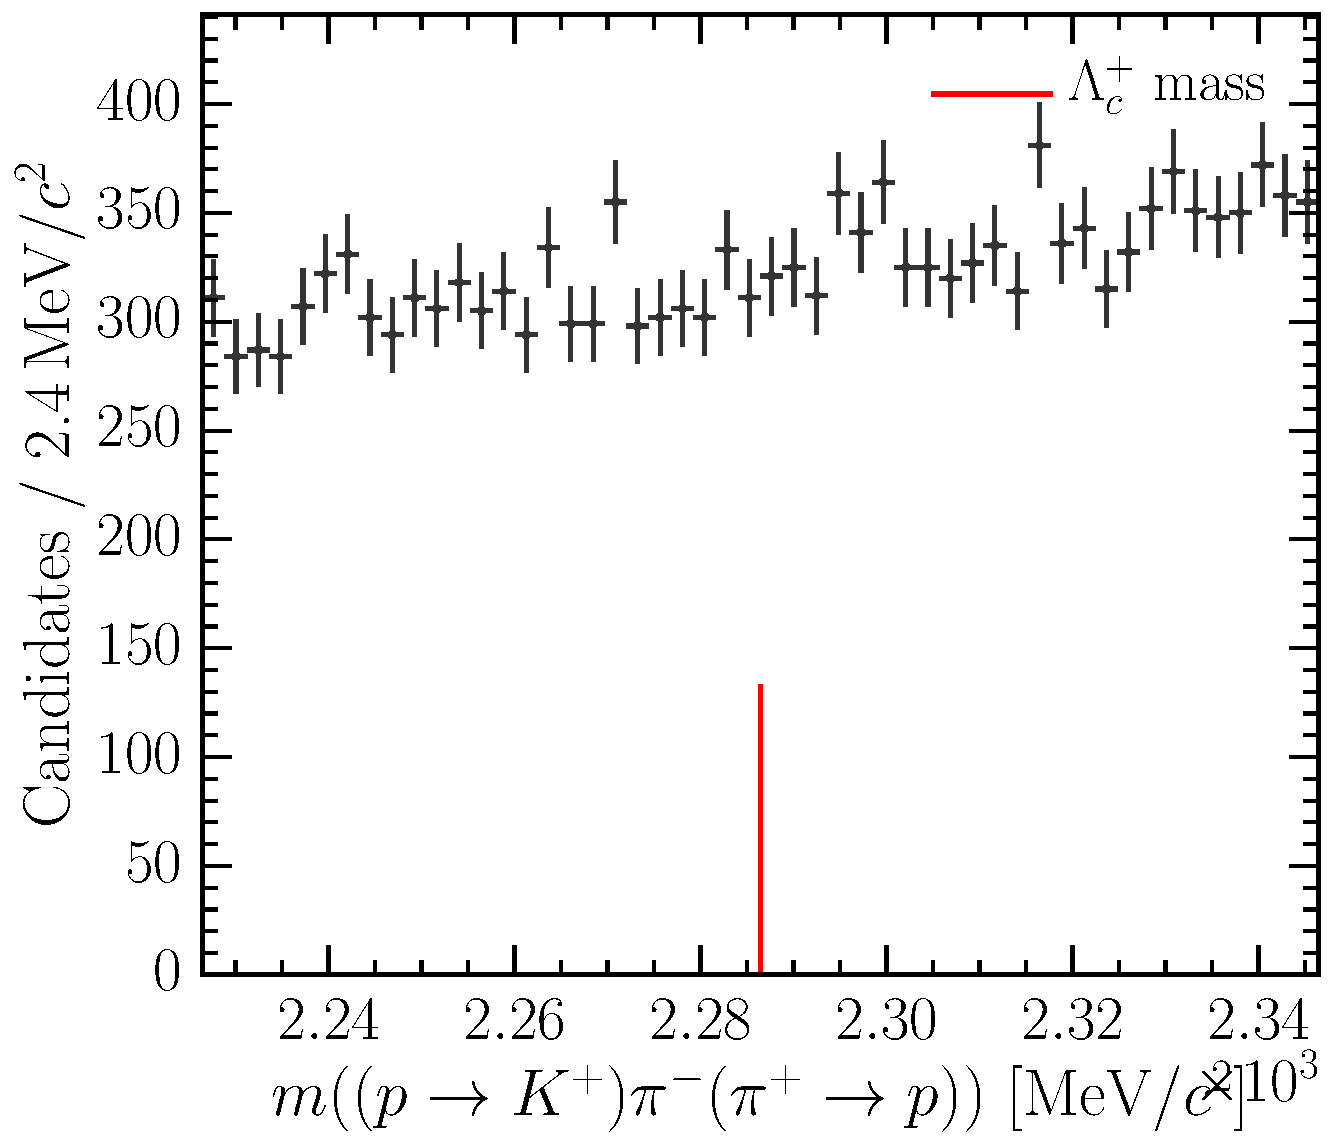
\includegraphics[width=\textwidth]{figures/cpv/selection/background_study/ppipi/LcToppipi_2012_MagDown_Lc_ppTokp_pim_pipTopp}
    \caption{\decay{\PLambdac}{\PKplus\Ppiminus\Pproton}}
    \label{fig:cpv:selection:background_study:ppipi_baryon:kpip}
  \end{subfigure}
  \begin{subfigure}[b]{0.3\textwidth}
    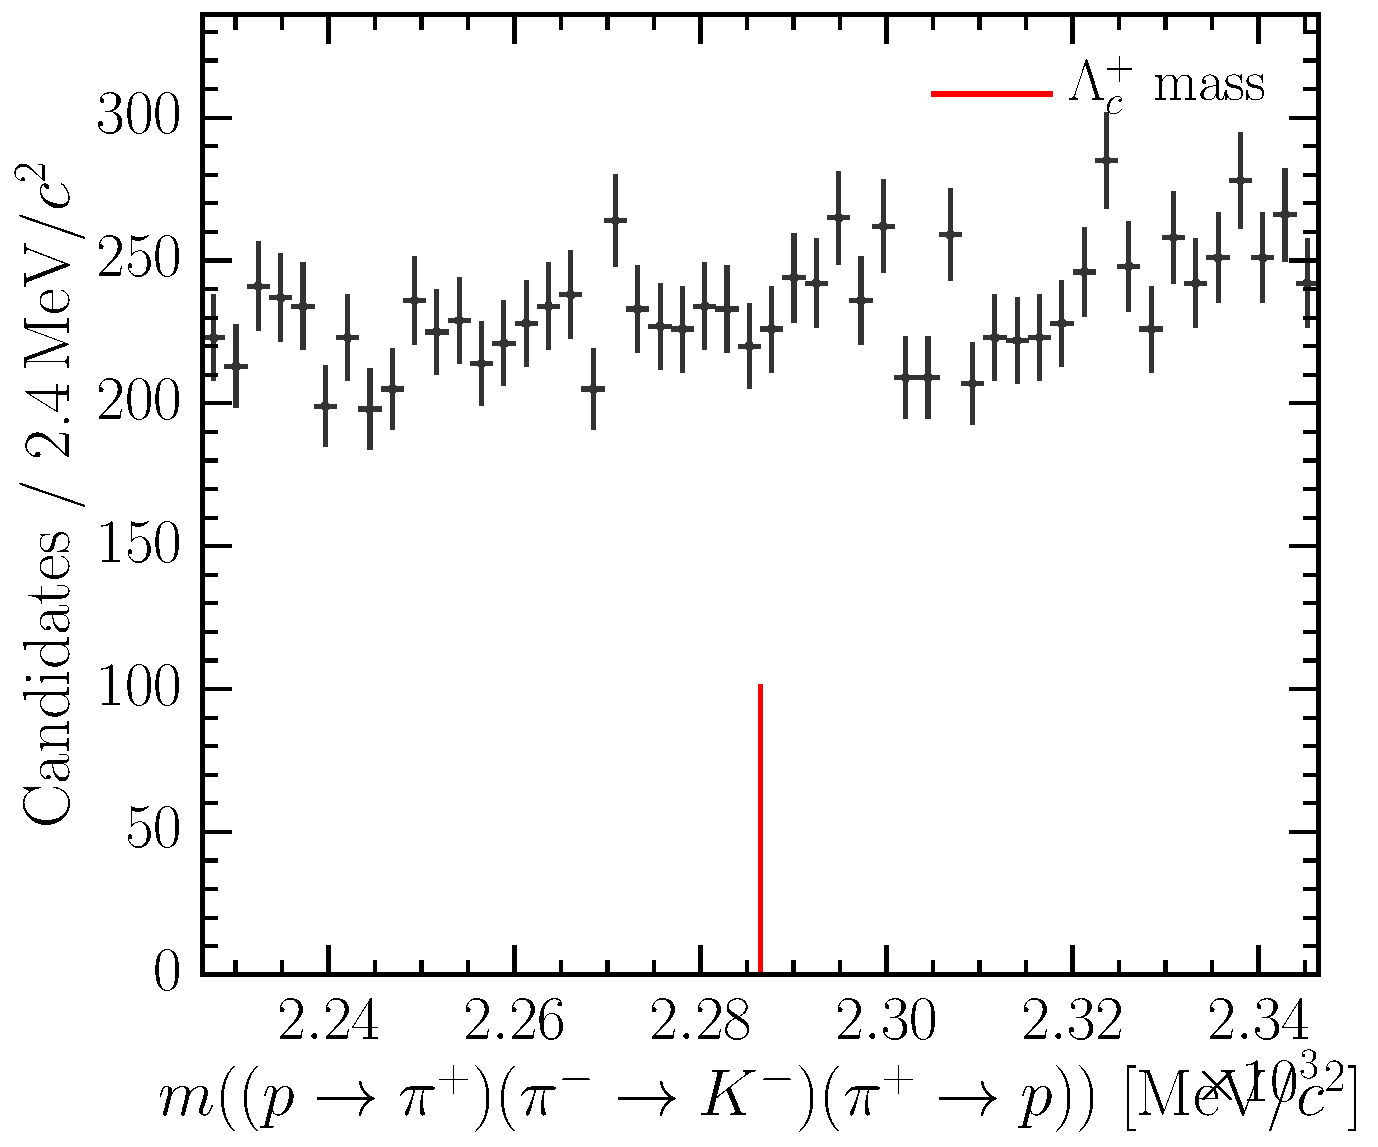
\includegraphics[width=\textwidth]{figures/cpv/selection/background_study/ppipi/LcToppipi_2012_MagDown_Lc_ppTopip_pimTokm_pipTopp}
    \caption{\decay{\PLambdac}{\Ppiplus\PKminus\Pproton}}
    \label{fig:cpv:selection:background_study:ppipi_baryon:pikp}
  \end{subfigure}
  \begin{subfigure}[b]{0.3\textwidth}
    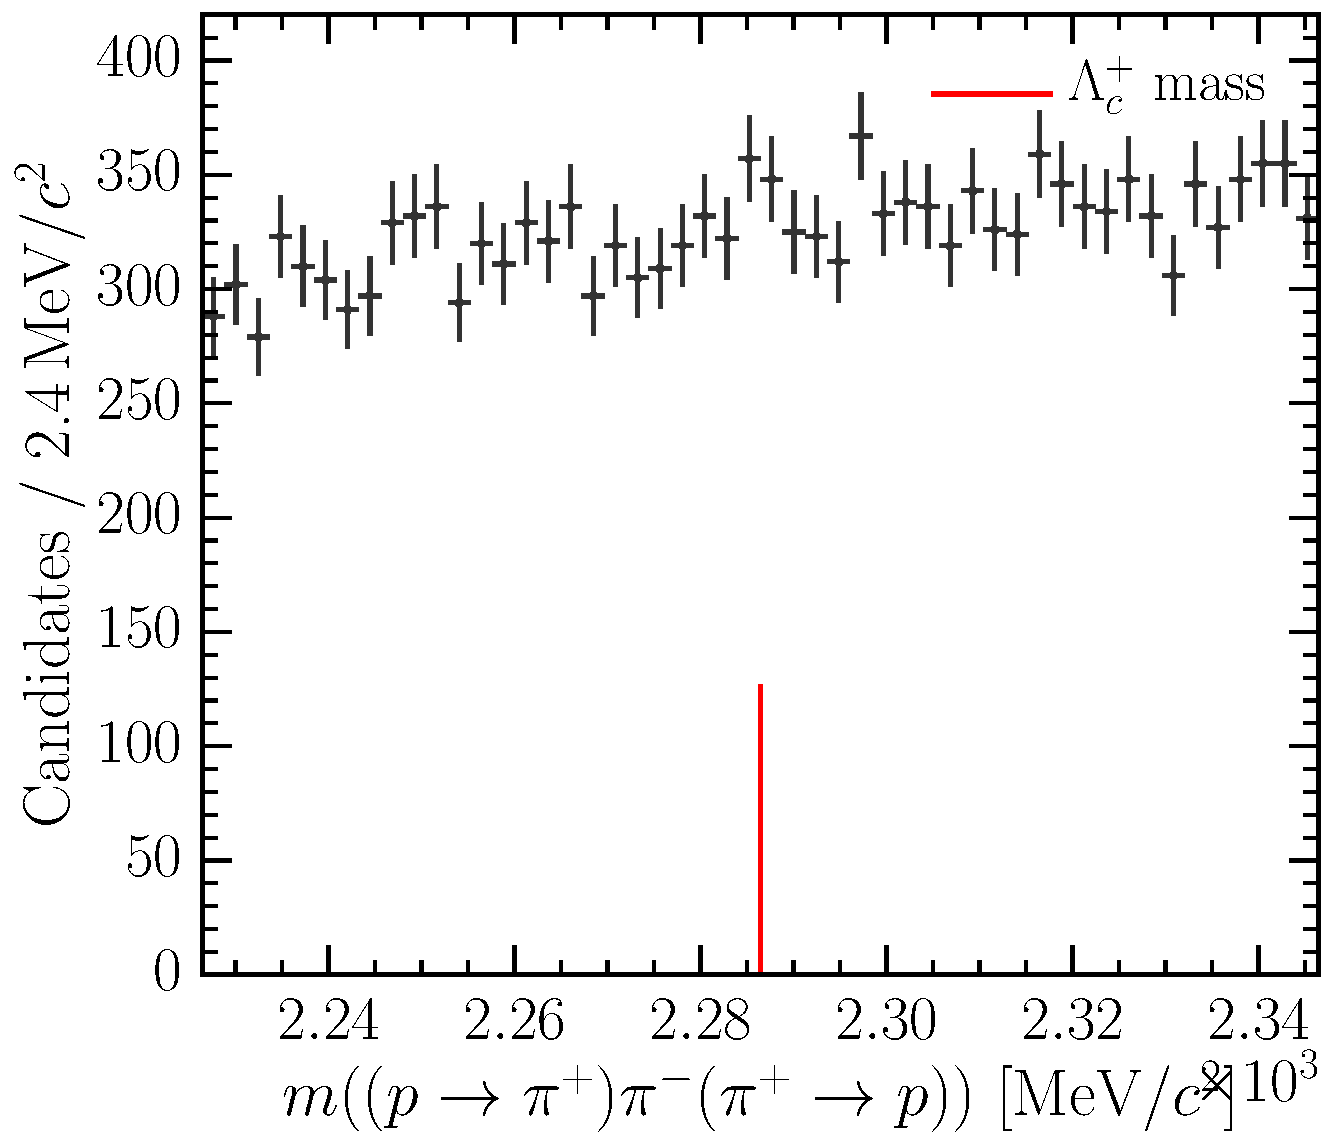
\includegraphics[width=\textwidth]{figures/cpv/selection/background_study/ppipi/LcToppipi_2012_MagDown_Lc_ppTopip_pim_pipTopp}
    \caption{\decay{\PLambdac}{\Ppiplus\Ppiminus\Pproton}}
    \label{fig:cpv:selection:background_study:ppipi_baryon:pipip}
  \end{subfigure}
  \begin{subfigure}[b]{0.3\textwidth}
    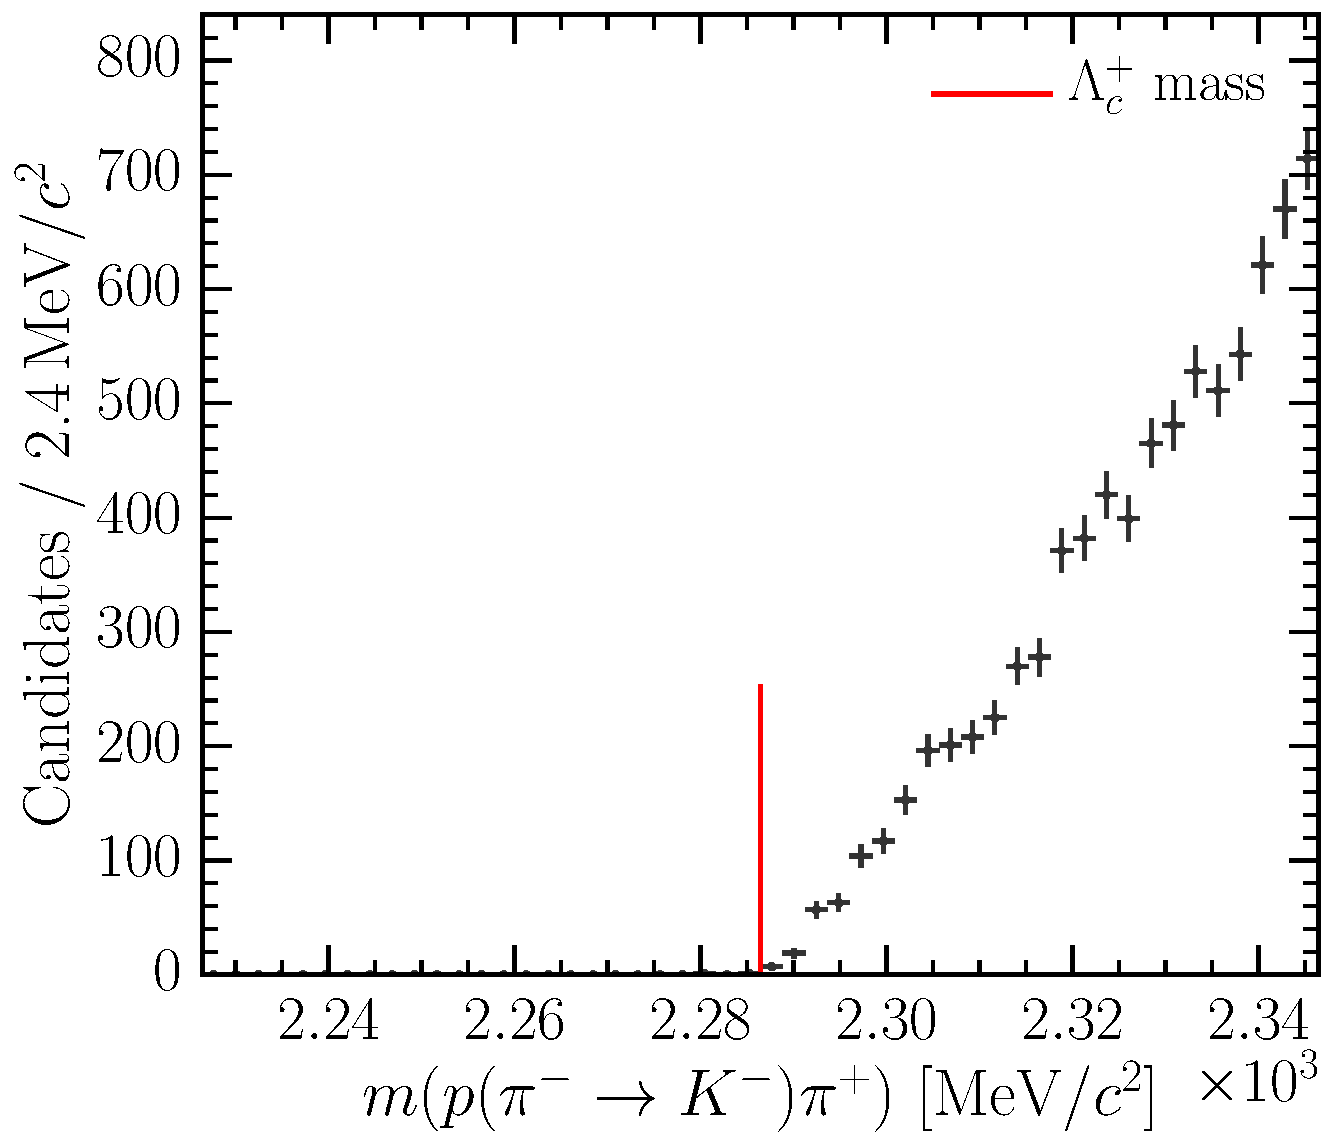
\includegraphics[width=\textwidth]{figures/cpv/selection/background_study/ppipi/LcToppipi_2012_MagDown_Lc_pp_pimTokm_pip}
    \caption{\decay{\PLambdac}{\Pproton\PKminus\Ppiplus}}
    \label{fig:cpv:selection:background_study:ppipi_baryon:pkpi}
  \end{subfigure}
  \begin{subfigure}[b]{0.3\textwidth}
    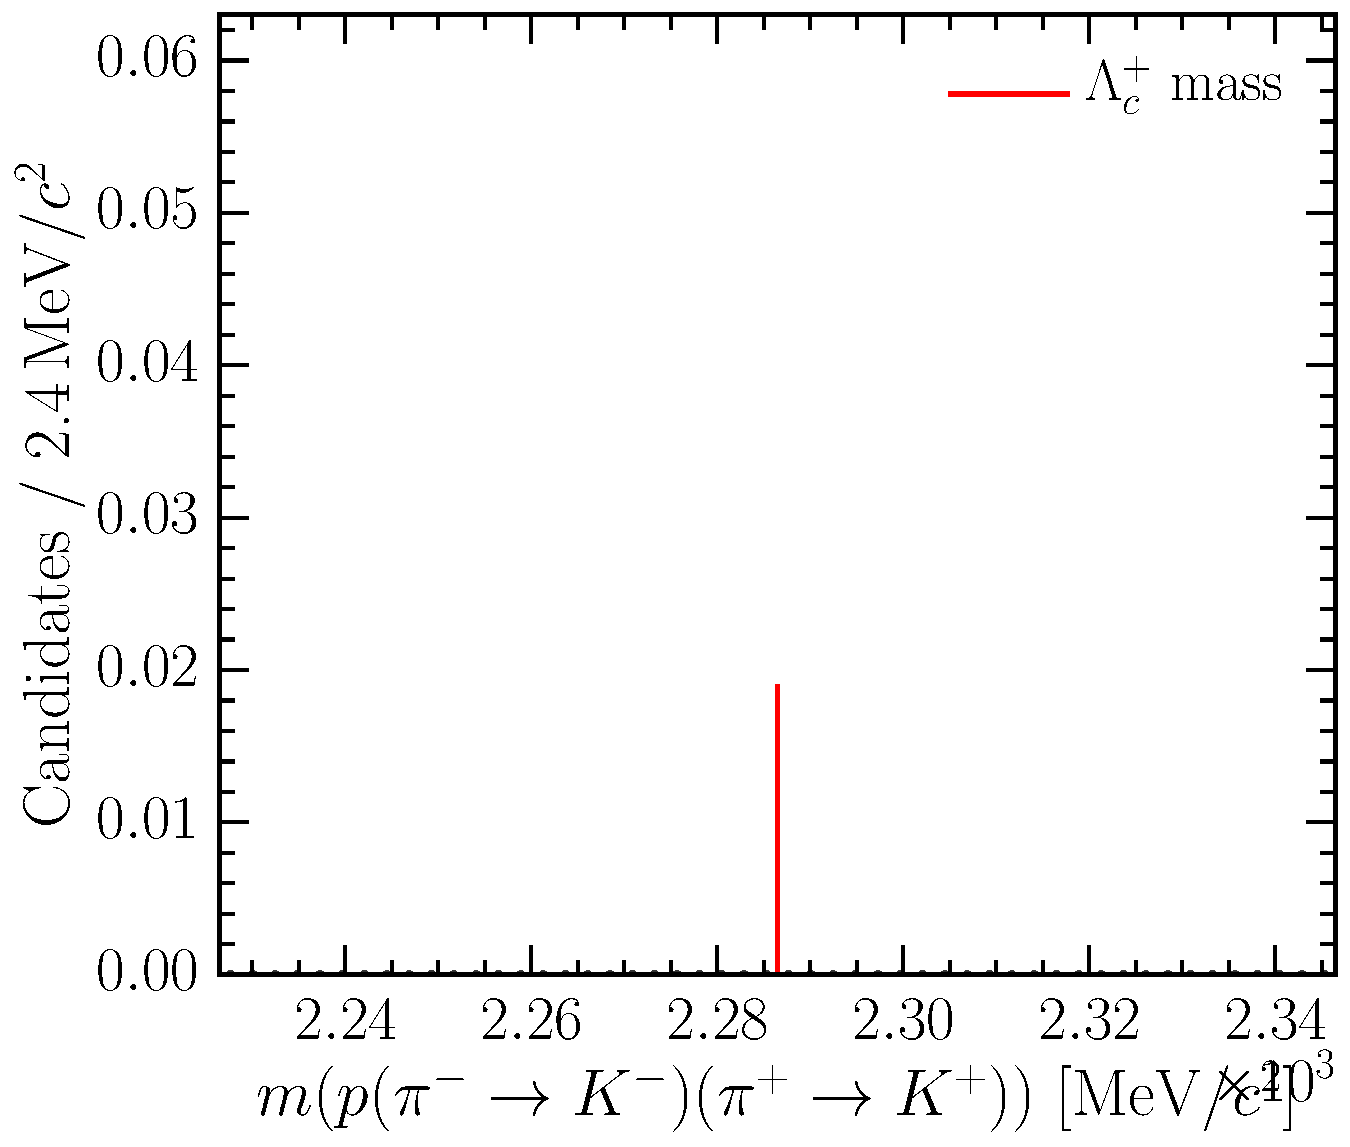
\includegraphics[width=\textwidth]{figures/cpv/selection/background_study/ppipi/LcToppipi_2012_MagDown_Lc_pp_pimTokm_pipTokp}
    \caption{\decay{\PLambdac}{\Pproton\PKminus\PKplus}}
    \label{fig:cpv:selection:background_study:ppipi_baryon:pkk}
  \end{subfigure}
  \begin{subfigure}[b]{0.3\textwidth}
    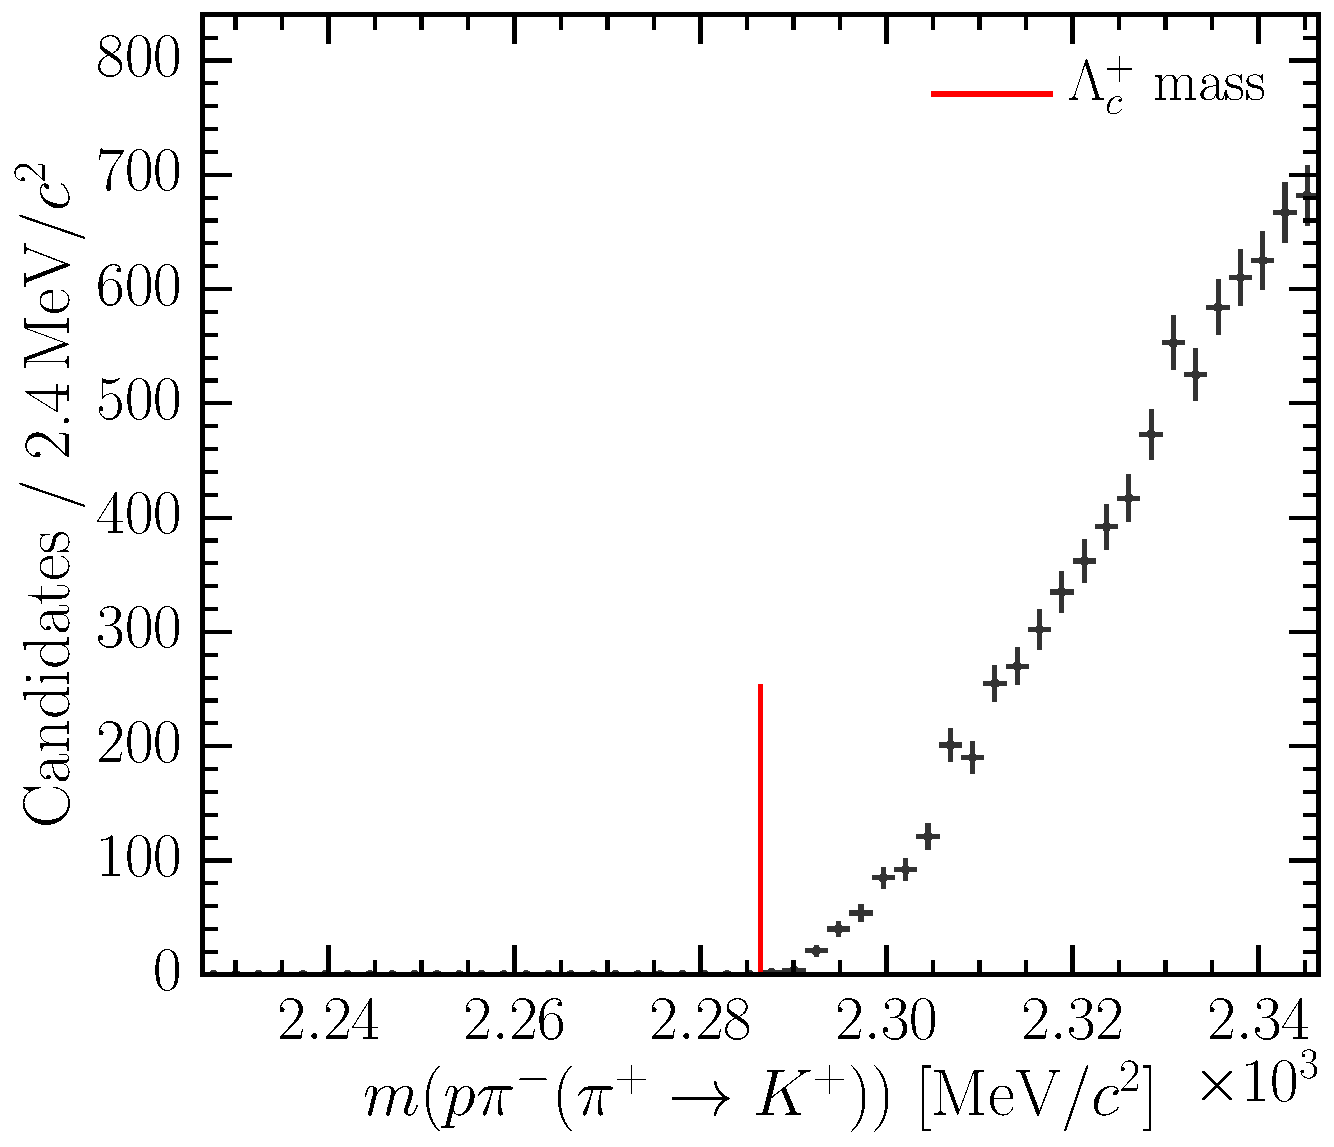
\includegraphics[width=\textwidth]{figures/cpv/selection/background_study/ppipi/LcToppipi_2012_MagDown_Lc_pp_pim_pipTokp}
    \caption{\decay{\PLambdac}{\Pproton\Ppiminus\PKplus}}
    \label{fig:cpv:selection:background_study:ppipi_baryon:ppik}
  \end{subfigure}
  \caption{%
    Wrong-mass distributions obtained when changing the mass hypotheses of the
    fully selected \PLambdac\ children in the \ppipi\ mode, where one child is
    assigned the proton mass hypothesis.
    The $x$-axis on each sub-figure shows the substitutions that have been
    made.
    For example, the ${\Pproton(\Ppiminus \to \PKminus)\Ppiplus}$ distribution is where the
    nominal proton candidate has been assigned the pion mass hypothesis, and
    the nominal pion with opposite charge to the proton has been also assigned
    the kaon hypothesis.
    The vertical red lines indicate the nominal mass of the misidentified 
    particle under study.
    Only the 2012 magnet down data is shown.
  }
  \label{fig:cpv:selection:background_study:ppipi_baryon}
\end{figure}

\begin{figure}
  \begin{subfigure}[b]{0.5\textwidth}
    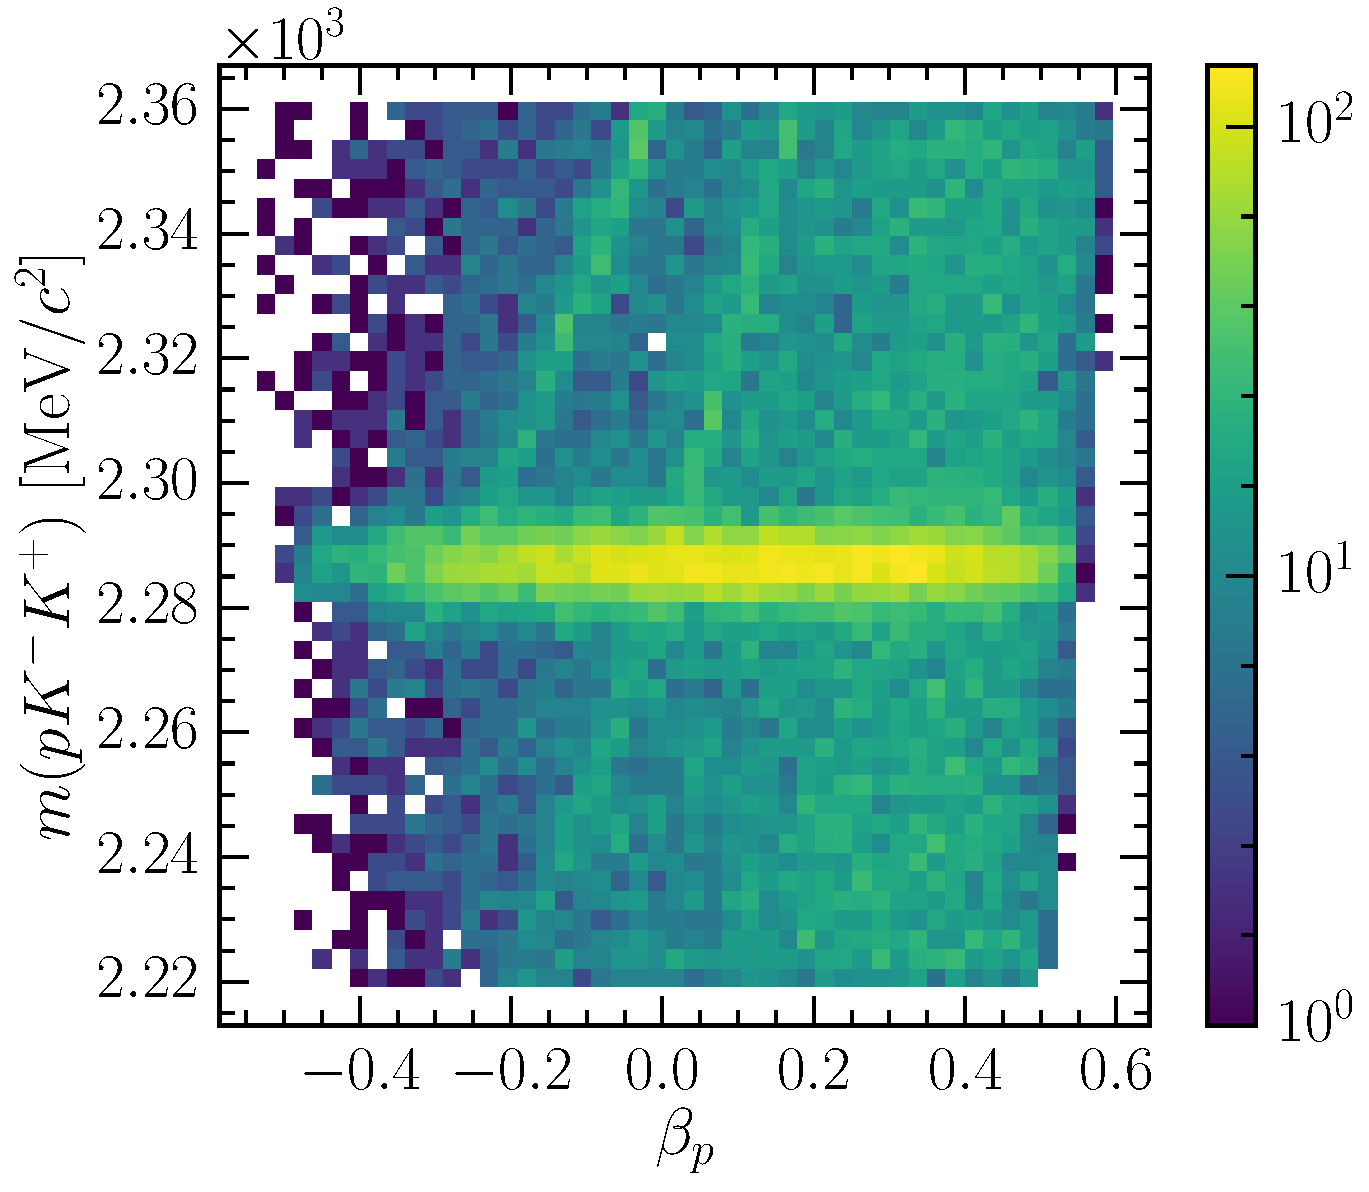
\includegraphics[width=\textwidth]{cpv/selection/background_study/pKK/LcTopKK_2012_MagDown_beta_p-Lb_DTF_Lc_M}
    \caption{Before mis-ID vetoes}
    \label{fig:cpv:selection:background_study:mom_asym:pKK:before}
  \end{subfigure}
  \begin{subfigure}[b]{0.5\textwidth}
    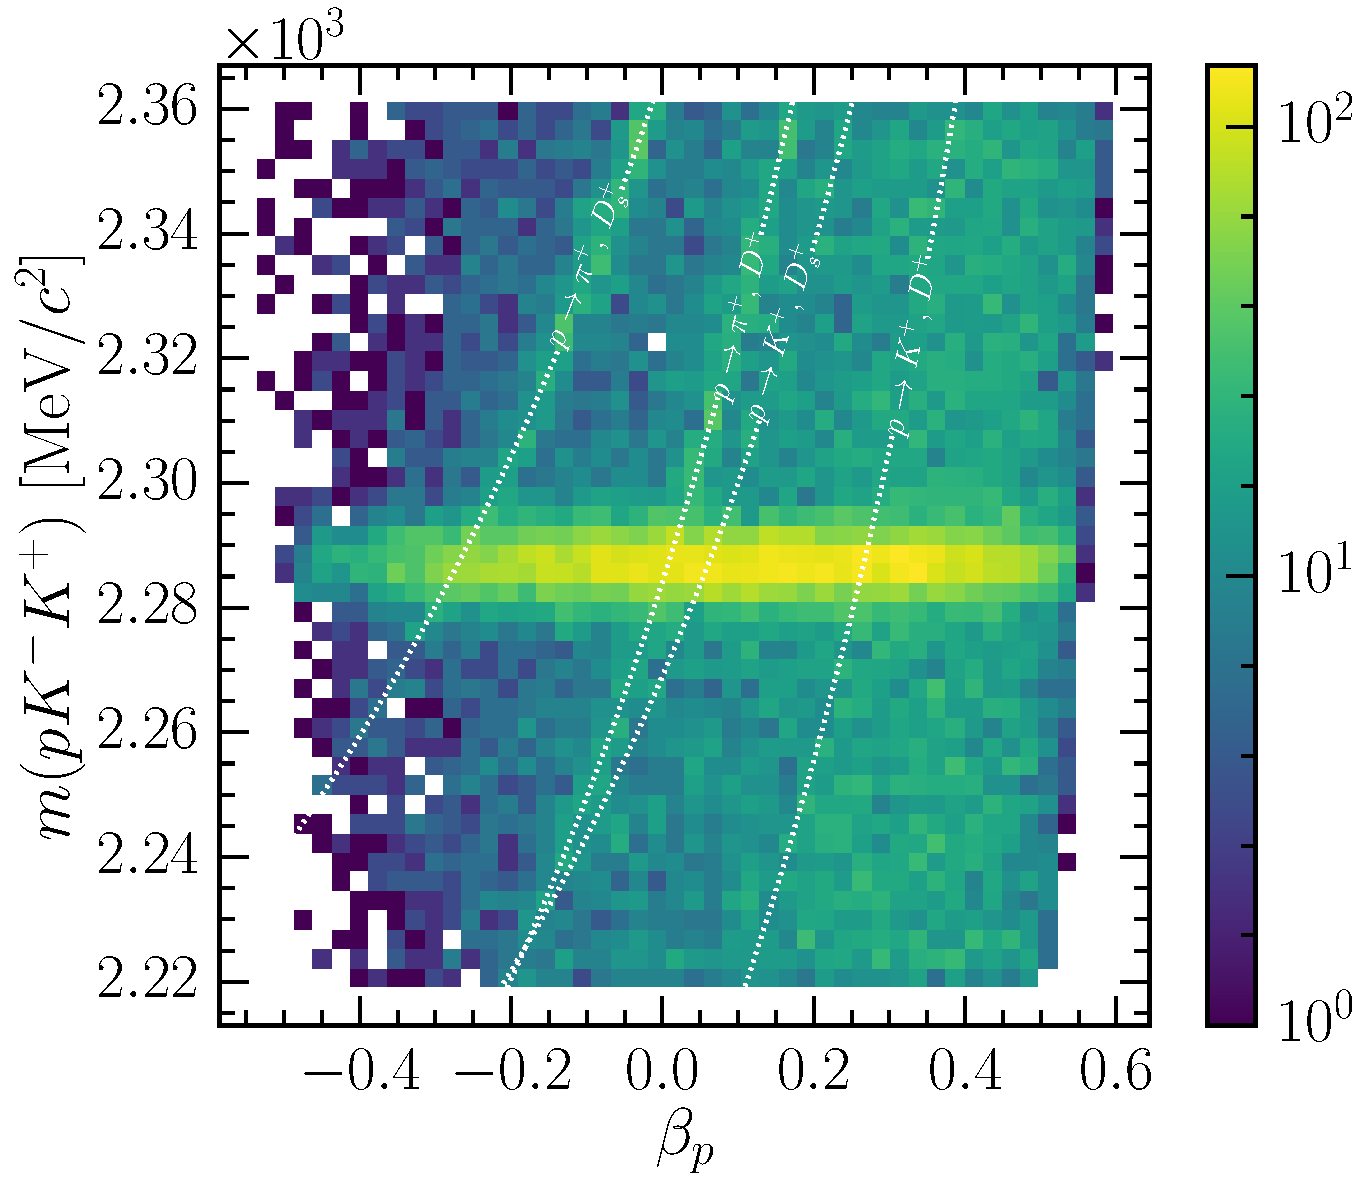
\includegraphics[width=\textwidth]{cpv/selection/background_study/pKK/LcTopKK_2012_MagDown_beta_p-Lb_DTF_Lc_M_contours}
    \caption{With theoretical contours}
    \label{fig:cpv:selection:background_study:mom_asym:pKK:contours}
  \end{subfigure}
  \begin{subfigure}[b]{0.5\textwidth}
    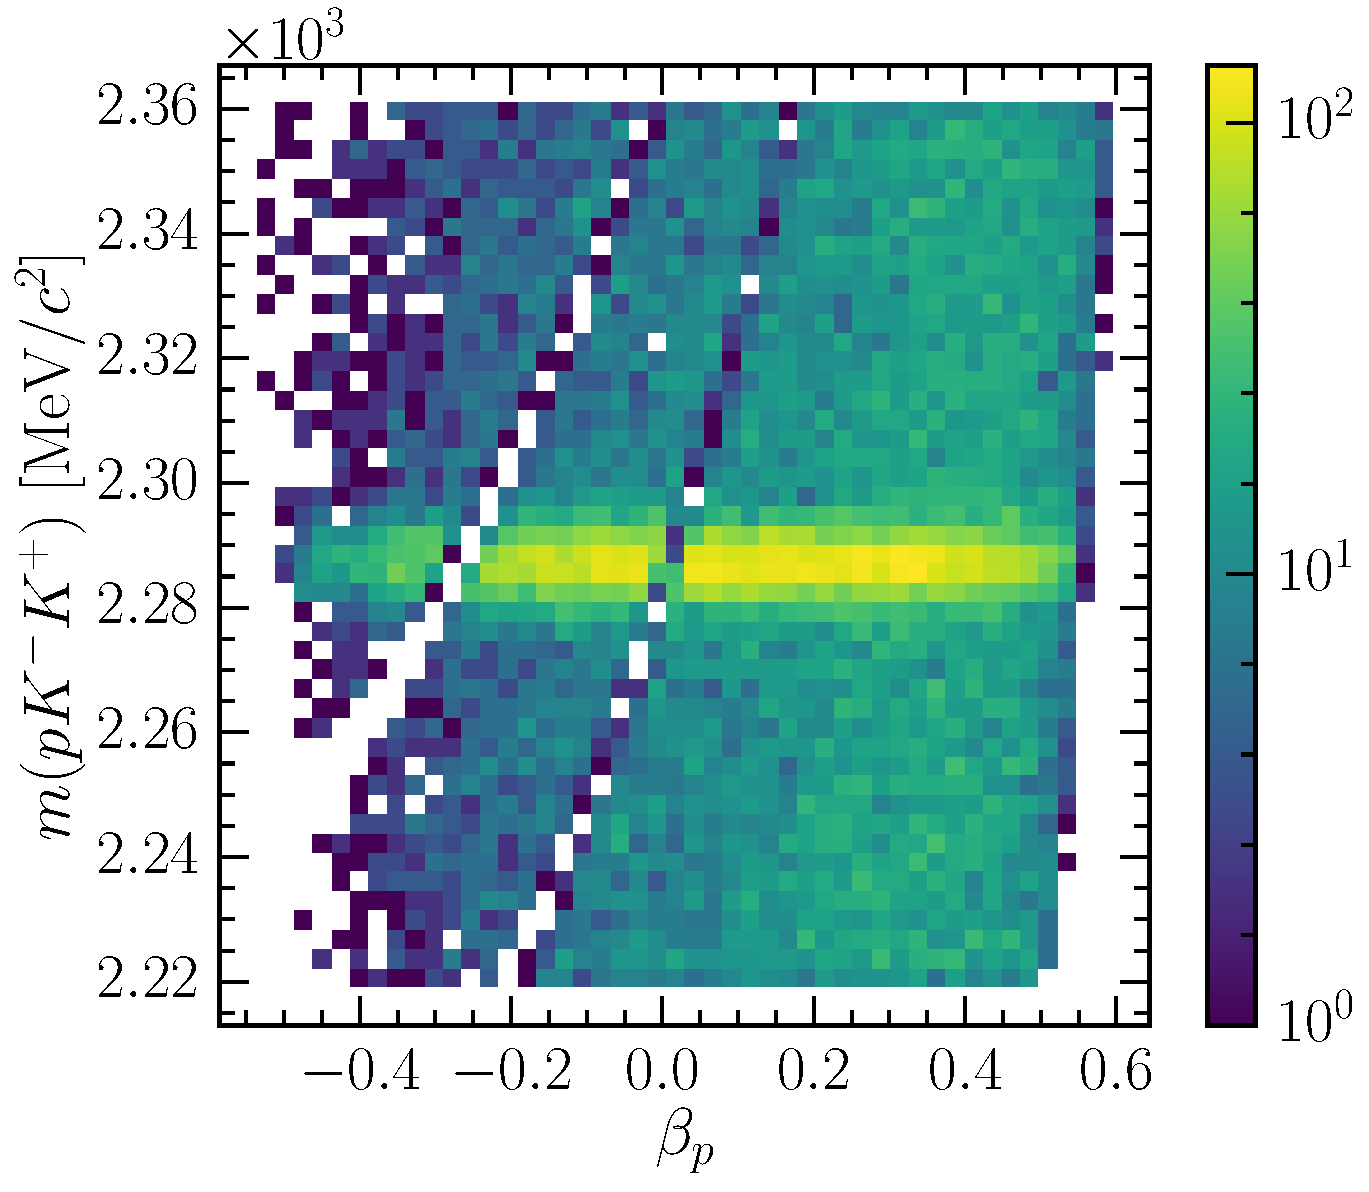
\includegraphics[width=\textwidth]{cpv/selection/background_study/pKK/LcTopKK_2012_MagDown_beta_p-Lb_DTF_Lc_M-vetoes}
    \caption{After mis-ID vetoes}
    \label{fig:cpv:selection:background_study:mom_asym:pKK:after}
  \end{subfigure}
  \caption{%
    Plane of $\beta_{\Pproton}$--$m(\PLambdac)$ for the \pKK\ mode in the 2012
    magnet down dataset.
    The ``theoretical contours'' shown on
    \cref{fig:cpv:selection:background_study:mom_asym:pKK:contours} are the
    solution of the parametric equation that defines the relationship between
    $m(\PLambdac)$, $\beta_{\Pproton}$, and the mass of the misidentified
    particle decaying to a particular final state.
    The plane after the misidentification vetoes, defined in
    \cref{chap:cpv:selection:background_study:mass_hypo}, is shown in
    \cref{fig:cpv:selection:background_study:mom_asym:pKK:after}.
  }
  \label{fig:cpv:selection:background_study:mom_asym:pKK}
\end{figure}

\begin{figure}
  \begin{subfigure}[b]{0.5\textwidth}
    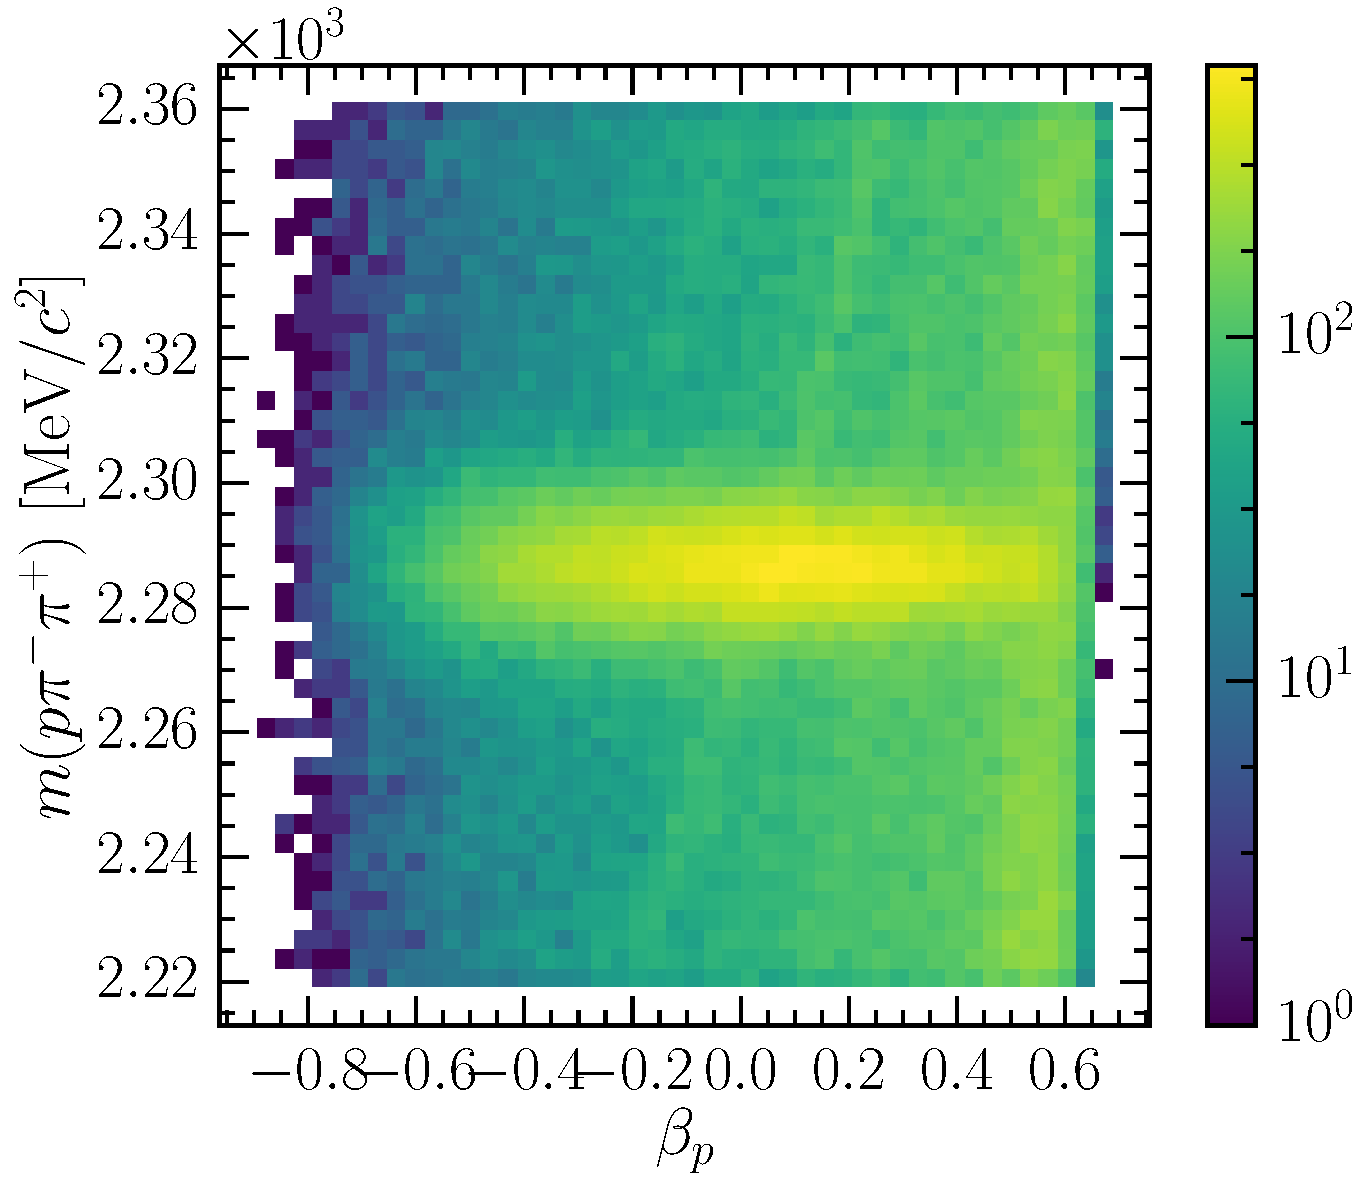
\includegraphics[width=\textwidth]{cpv/selection/background_study/ppipi/LcToppipi_2012_MagDown_beta_p-Lb_DTF_Lc_M}
    \caption{Before mis-ID vetoes}
    \label{fig:cpv:selection:background_study:mom_asym:ppipi:before}
  \end{subfigure}
  \begin{subfigure}[b]{0.5\textwidth}
    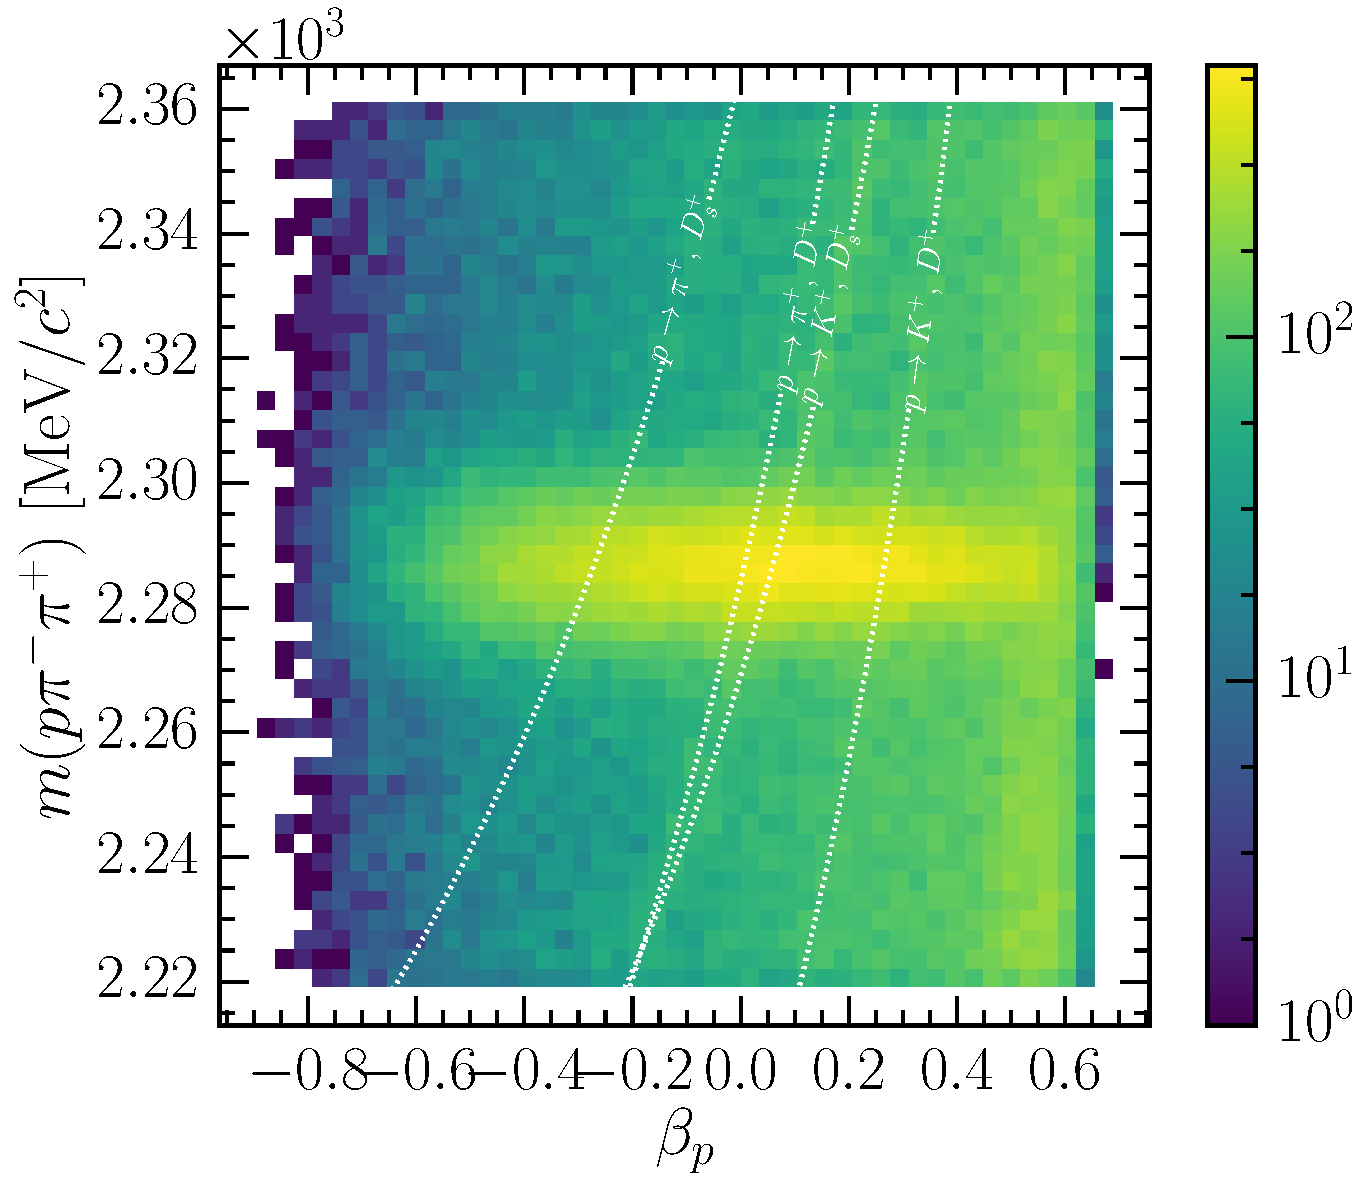
\includegraphics[width=\textwidth]{cpv/selection/background_study/ppipi/LcToppipi_2012_MagDown_beta_p-Lb_DTF_Lc_M_contours}
    \caption{With theoretical contours}
    \label{fig:cpv:selection:background_study:mom_asym:ppipi:contours}
  \end{subfigure}
  \begin{subfigure}[b]{0.5\textwidth}
    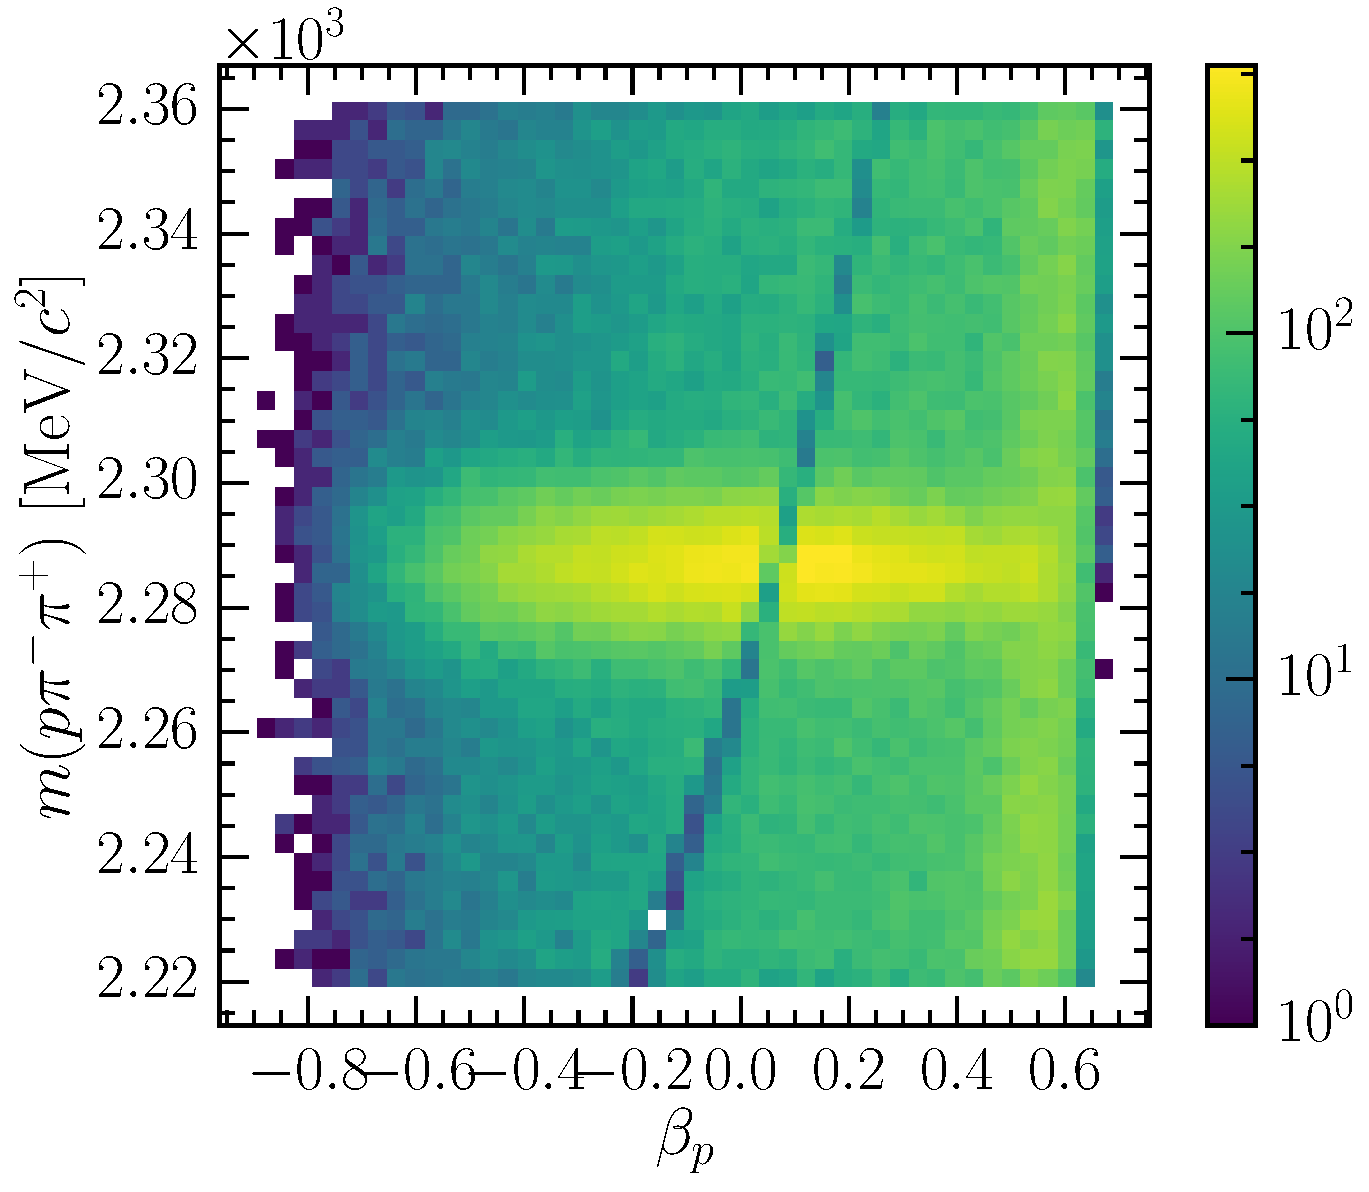
\includegraphics[width=\textwidth]{cpv/selection/background_study/ppipi/LcToppipi_2012_MagDown_beta_p-Lb_DTF_Lc_M-vetoes}
    \caption{After mis-ID vetoes}
    \label{fig:cpv:selection:background_study:mom_asym:ppipi:after}
  \end{subfigure}
  \caption{%
    Plane of $\beta_{\Pproton}$--$m(\PLambdac)$ for the \ppipi\ mode in the
    2012 magnet down dataset.
    The ``theoretical contours'' shown on
    \cref{fig:cpv:selection:background_study:mom_asym:ppipi:contours} are the
    solution of the parametric equation that defines the relationship between
    $m(\PLambdac)$, $\beta_{\Pproton}$, and the mass of the misidentified
    particle decaying to a particular final state.
    The plane after the misidentification vetoes, defined in
    \cref{chap:cpv:selection:background_study:mass_hypo}, is shown in
    \cref{fig:cpv:selection:background_study:mom_asym:ppipi:after}.
  }
  \label{fig:cpv:selection:background_study:mom_asym:ppipi}
\end{figure}

\section{Multiple candidates}
\label{chap:cpv:selection:multiple_candidates}

It is possible, but unlikely, that two or more true \LcTophh\ decays are
reconstructed in a single \ac{LHC} bunch crossing.
It is more likely that such multiple candidates are caused by unphysical means,
such as cloned tracks~\cite{LHCb-INT-2011-009}.
In the case where an event has multiple \PLambdac\ candidates, one is selected
at random for further analysis and the rest are discarded.
The fractions of events containing multiple \PLambdac\ candidates are given in
\cref{tab:cpv:selection:multiple_candidates:pKK,tab:cpv:selection:multiple_candidates:ppipi}.

\begin{table}
  \caption{%
    Statistics on multiple candidates in the \pKK\ data.
    The total number of events $N_{\text{Events}}$ is the number of
    proton-proton collisions that make up the data sub-sample, and
    $N_{\text{Candidates}}$ is the number of \PLambdac\ candidates.
    The fraction of events containing at least two candidates is
    $f_{\text{Multiple}}$, and the fraction of those events that fall within
    the signal window in the \PLambdac\ mass distribution is
    $f_{\text{Multiple, sig.}}$.
  }
  \label{tab:cpv:selection:multiple_candidates:pKK}
  \begin{tabular}{ccccccc}
  \toprule
  Year & Polarity & $N_{\text{Events}}$ & $N_{\text{Candidates}}$ & $f_{\text{Multiple}}$ [\si{\percent}] & $f_{\text{Multiple, sig.}}$ [\si{\percent}] \\
  \midrule
2011   & Down     & $11600 \pm 100$     & $11800 \pm 100$         & $1.39 \pm 0.11$                       & $0.16 \pm 0.06$                             \\
2011   & Up       & $8300 \pm 100$      & $8400 \pm 100$          & $1.62 \pm 0.14$                       & $0.39 \pm 0.10$                             \\
2012   & Down     & $26900 \pm 200$     & $27300 \pm 200$         & $1.51 \pm 0.08$                       & $0.23 \pm 0.04$                             \\
2012   & Up       & $26900 \pm 200$     & $27400 \pm 200$         & $1.65 \pm 0.08$                       & $0.28 \pm 0.05$                             \\
  \bottomrule
\end{tabular}

\end{table}

\begin{table}
  \caption{%
    Multiple candidates for the \ppipi\ data.
    The total number of events $N_{\text{Events}}$ is the number of
    proton-proton collisions that make up the data sub-sample, and
    $N_{\text{Candidates}}$ is the number of \PLambdac\ candidates.
    The fraction of events containing at least two candidates is
    $f_{\text{Multiple}}$, and the fraction of those events that fall within
    the signal window in the \PLambdac\ mass distribution is
    $f_{\text{Multiple, sig.}}$.
  }
  \label{tab:cpv:selection:multiple_candidates:ppipi}
  \begin{tabular}{ccccccc}
  \toprule
  Year & Polarity & $N_{\text{Events}}$ & $N_{\text{Candidates}}$ & $f_{\text{Multiple}}$ [\si{\percent}] & $f_{\text{Multiple, sig.}}$ [\si{\percent}] \\
  \midrule
2011   & Down     & $64700 \pm 300$     & $65800 \pm 300$         & $1.62 \pm 0.05$                       & $0.23 \pm 0.03$                             \\
2011   & Up       & $46800 \pm 200$     & $47600 \pm 200$         & $1.80 \pm 0.06$                       & $0.32 \pm 0.04$                             \\
2012   & Down     & $163100 \pm 400$    & $166100 \pm 400$        & $1.75 \pm 0.03$                       & $0.29 \pm 0.02$                             \\
2012   & Up       & $161900 \pm 400$    & $165000 \pm 400$        & $1.80 \pm 0.03$                       & $0.32 \pm 0.02$                             \\
  \bottomrule
\end{tabular}

\end{table}
